%----------------------------------------------------------------------------------------
% PACKAGES AND OTHER DOCUMENT CONFIGURATIONS
%----------------------------------------------------------------------------------------

% !TEX encoding = UTF-8
% !TEX TS-program = pdflatex
% !TEX root = computabilità e algoritmi.tex
% !TEX spellcheck = it-IT

\documentclass[a4paper, 11pt]{report} % Font size (can be 10pt, 11pt or 12pt) and paper size (remove a4paper for US letter paper)
\usepackage[italian]{babel}      							% Lingua italiana
\usepackage[margin=.9in]{geometry}             % Imposta i margini del documento

\usepackage[T1]{fontenc} % Required for accented characters
\usepackage[mathletters]{ucs}    % Caratteri matematici come UTF8
\usepackage[utf8,utf8x]{inputenc}      % Ancora utf8

\usepackage{eurosym}                %simbolo dell'euro
\usepackage{listings}
\usepackage[usenames,dvipsnames,svgnames,table]{xcolor}
% Imposta lo spazio nella list of listing in modo simile alla list of figures/tables
%\makeatletter
%\let\my@chapter\@chapter
%\renewcommand*{\@chapter}{%
%  \addtocontents{lol}{\protect\addvspace{10pt}}%
%  \my@chapter}
%\makeatother


\definecolor{codegreen}{rgb}{0,0.6,0}
\definecolor{codegray}{rgb}{0.5,0.5,0.5}
\definecolor{backcolor}{rgb}{0.98,0.98,0.98}

\renewcommand{\lstlistingname}{Codice}% Listing -> codice
\renewcommand{\lstlistlistingname}{Elenco dei frammenti di codice}% List of Listings -> Frammenti di codice

\lstdefinestyle{mystyle}{
    backgroundcolor=\color{backcolor},   
    commentstyle=\color{Peach}\ttfamily,
    keywordstyle=\color{RoyalBlue},
    numberstyle=\tiny\color{codegray},
    stringstyle=\color{SeaGreen}\ttfamily,
    basicstyle=\footnotesize\ttfamily,
    breakatwhitespace=false,         
    breaklines=true,                 
    captionpos=b,                    
    keepspaces=true,                 
    numbers=left,                    
    numbersep=5pt,                  
    showspaces=false,                
    showstringspaces=false,
    showtabs=false,                  
    tabsize=2,
    frame=trbl, % draw a frame at the top, right, left and bottom of the listing
	frameround=ftff, % angolo in basso a destro curvo
	framesep=4pt, % quarter circle size of the round corners,
	inputencoding=utf8,
    extendedchars=true,
    literate={á}{{\'a}}1 {à}{{\`a}}1 {é}{{\'e}}1 {è}{{\`e}}1 {ù}{{\`u}}1 {ò}{{\`o}}1 {ì}{{\`i}}1,
    belowskip=1em,
    aboveskip=1em,
}

 
\lstset{style=mystyle}

\lstdefinelanguage{JavaScript}
{
  % list of keywords
  morekeywords={ true, false, catch, function, break,	new, class, extends, var, require, switch, return, import, if, while, for, this, View, Text, StyleSheet},
  sensitive=false, % keywords are not case-sensitive
  morecomment=[l]{//}, % l is for line comment
  morecomment=[s]{/*}{*/}, % s is for start and end delimiter
  morestring=[b]' % defines that strings are enclosed in double quotes
}

\lstdefinelanguage{JSON}
{
  % list of keywords
  morekeywords={string, boolean, int, Array, Node, Asset, AssetDetail, Filter, FilterItem},
  sensitive=false, % keywords are not case-sensitive
  morecomment=[l]{//}, % l is for line comment
  morecomment=[s]{/*}{*/}, % s is for start and end delimiter
  morestring=[b]" % defines that strings are enclosed in double quotes
}

\lstdefinelanguage{URM}
{
	% list of keywords
	morekeywords={ S, J, T, Z, I},
	sensitive=false, % keywords are not case-sensitive
	morecomment=[l]{//}, % l is for line comment
	morecomment=[s]{/*}{*/}, % s is for start and end delimiter
	morestring=[b]' % defines that strings are enclosed in double quotes
}

\lstdefinelanguage{RDFA}{
	language=html,
	sensitive=true, 
	alsoletter={<>=-},
	ndkeywords={
		% General
		=,
		% HTML attributes
		charset=, id=, width=, height=, property=, about=, rel=, rev=, prefix=, vocab=, content=, datatype=
	},  
	morecomment=[s]{<!--}{-->},
	tag=[s]
}

%\tightlist per compatibilità con pandoc
\providecommand{\tightlist}{%
  \setlength{\itemsep}{0pt}\setlength{\parskip}{0pt}}


\usepackage[labelfont=bf]{caption}

\usepackage[protrusion=true,expansion=true]{microtype} % Better typography
\usepackage{graphicx} % Required for including pictures
\usepackage{wrapfig} % Allows in-line images


\usepackage{subfig}
\usepackage{hyperref}
\usepackage{mathpazo} % Use the Palatino font

\linespread{1.05} % Change line spacing here, Palatino benefits from a slight increase by default
\usepackage{placeins}
\usepackage{sourcecodepro}
\usepackage{hyperref}                   % collegamenti ipertestuali

\usepackage[colorinlistoftodos,prependcaption]{todonotes} %todo

\usepackage{amsmath}
\usepackage{mathtools}

\usepackage{float}
\usepackage{algorithm}
\usepackage{algpseudocode} % https://en.wikibooks.org/wiki/LaTeX/Algorithms#Typesetting_using_the_algorithmicx_package
\usepackage{amssymb}  %$\mathbb{N}$ per il simbolo dei numeri naturali 

\usepackage{enumerate} % permette di personalizzare enumerate

\makeatletter
\renewcommand\@biblabel[1]{\textbf{#1.}} % Change the square brackets for each bibliography item from '[1]' to '1.'
\renewcommand{\@listI}{\itemsep=0pt} % Reduce the space between items in the itemize and enumerate environments and the bibliography

\renewcommand{\maketitle}{ % Customize the title - do not edit title and author name here, see the TITLE block below
\begin{flushright} % Right align
{\LARGE\@title} % Increase the font size of the title

\vspace{50pt} % Some vertical space between the title and author name

{\large\@author} % Author name
\\\@date % Date

\vspace{100pt} % Some vertical space between the author block and abstract
\end{flushright}
}

%% breakablealgorithm http://tex.stackexchange.com/questions/33866/algorithm-tag-and-page-break
\makeatletter
\newenvironment{breakablealgorithm}
{% \begin{breakablealgorithm}
	\begin{center}
		\refstepcounter{algorithm}% New algorithm
		\hrule height.8pt depth0pt \kern2pt% \@fs@pre for \@fs@ruled
		\renewcommand{\caption}[2][\relax]{% Make a new \caption
			{\raggedright\textbf{\ALG@name~\thealgorithm} ##2\par}%
			\ifx\relax##1\relax % #1 is \relax
			\addcontentsline{loa}{algorithm}{\protect\numberline{\thealgorithm}##2}%
			\else % #1 is not \relax
			\addcontentsline{loa}{algorithm}{\protect\numberline{\thealgorithm}##1}%
			\fi
			\kern2pt\hrule\kern2pt
		}
	}{% \end{breakablealgorithm}
	\kern2pt\hrule\relax% \@fs@post for \@fs@ruled
\end{center}
}
\makeatother

\makeatletter % trattino con punto sopra
\newcommand{\dotminus}{\mathbin{\text{\@dotminus}}}

\newcommand{\@dotminus}{%
	\ooalign{\hidewidth\raise1ex\hbox{.}\hidewidth\cr$\m@th-$\cr}%
}
\makeatother

\DeclarePairedDelimiter{\ceil}{\lceil}{\rceil}
\DeclarePairedDelimiter{\floor}{\lfloor}{\rfloor}

%----------------------------------------------------------------------------------------
% TITLE
%----------------------------------------------------------------------------------------

\title{\textbf{Computabilità e Algoritmi}\\ % Title
A.A. 2015-2016} % Subtitle

\author{\textsc{Giacomo Manzoli}
\\ 1130822 % Author
\\{\textit{Università degli Studi di Padova}}} % Institution

\date{\today} % Date

%----------------------------------------------------------------------------------------

\begin{document}

\maketitle % Print the title section

%----------------------------------------------------------------------------------------
% ABSTRACT AND KEYWORDS
%----------------------------------------------------------------------------------------

%\renewcommand{\abstractname}{Summary} % Uncomment to change the name of the abstract to something else

\clearpage
\tableofcontents
\listofalgorithms

%\hspace*{3,6mm}\textit{Keywords:} lorem , ipsum , dolor , sit amet , lectus % Keywords

\vspace{30pt} % Some vertical space between the abstract and first section

%----------------------------------------------------------------------------------------
% ESSAY BODY
%----------------------------------------------------------------------------------------
\clearpage

\part{Computabilità}
% !TEX encoding = UTF-8
% !TEX TS-program = pdflatex
% !TEX root = computabilità e algoritmi.tex
% !TEX spellcheck = it-IT
\chapter{Funzioni calcolabili e Modelli di calcolo}
\section{Introduzione}\label{lezione-1---computabilituxe0-e-algoritmi}

Ci sono dei problemi che non possono essere risolti in modo algoritmico,
come la terminazione o la prova di correttezza di un programma, lo studio di questi problemi prende il nome di teoria della computabilità.

In questa teoria non viene preso in considerazione il consumo di
risorse in modo che le dimostrazioni effettuate siano indipendenti dal
modello di calcolo adottato.

Notoriamente, i problemi appartengono a varie classi di difficoltà:

\begin{itemize}
\item
  \textbf{P}: problemi che possono essere risolti da un algoritmo in
  tempo polinomiale
\item
  \textbf{NP}: problemi che possono essere risolti in tempo polinomiale
  ma in modo non deterministico
\item
  \textbf{EXP}: problemi che possono essere risolti da un algoritmo in
  tempo esponenziale
\end{itemize}

\subsection{L'informatica e la computabilità}\label{linformatica-e-la-computabilituxe0}

\emph{Computer science is no more about computers tha astronomy is about
telescopes. Dijkstra}.

L'idea dell'informatica nasce dalla logica, ricercando un procedimento
generale (macchina) su base combinatoria per trovare tutte le verità.

Libro: \emph{Nigel Cutland ``Computability. An Introduction to Recursive
Function Theory'' Cambridge University Press}.

% !TEX encoding = UTF-8
% !TEX program = pdflatex
% !TEX root = MEMOC.tex
% !TEX spellcheck = it-IT

% 20 Ottobre 2016
% Section Modellazione di un problema
% Subsection Lettura dei giornali
% Subsubsection Modellazione

% esercizio delle costruzione della barca.
\subsection{Costruzione di una barca (Esercizio 3)}

La costruzione di una barca da diporto comporta il completamento delle operazioni indicate nella tabella che segue, che ne riporta anche la durata in giorni.

\begin{table}[htbp]
	\centering
	\begin{tabular}{ccc}
		\textbf{Operazione} & \textbf{Durata} & \textbf{Precedenze} \\ \hline
		A                   & 2               & nessuna             \\ 
		B                   & 4               & A                   \\ 
		C                   & 2               & A                   \\ 
		D                   & 5               & A                   \\ 
		E                   & 3               & B,C                 \\ 
		F                   & 3               & E                   \\ 
		G                   & 2               & E                   \\ 
		H                   & 7               & D,E,G               \\ 
		I                   & 4               & F,G                 \\ 
	\end{tabular}
\end{table}

Si consideri che alcune operazioni sono in alternativa. In particolare, bisogna eseguire solo una tra le operazioni B e C, e solo una tra le operazioni F e G. Inoltre, se si eseguono sia C che G, la durata dell'operazione I si allunga di 2 giorni.
La tabella indica anche, per ogni operazione, l'insieme delle precedenze (operazioni che devono essere completate prima di poter eseguire l'operazione stessa).
Scrivere un modello di programmazione lineare per decidere quali operazioni in alternativa eseguire, con l'obiettivo di minimizzare la durata complessiva delle operazioni di costruzione.

\subsubsection{Modellazione}

Le scelte in questo caso riguardano quali attività svolgere, tra quelle che possono essere eseguite in alternativa al fine di minimizzare il makespan.

Dal momento che si vuole minimizzare la durata, conviene scegliere dopo quanti giorni dall'inizio dei lavori deve terminare una determinata attività:

$$
t_i \quad \text{dopo quanti giorni termina l'attività }i \in A = \{A, \ldots, I \}
$$

\noindent Così risulta facile definire la funzione obiettivo

$$
\min z
$$

\noindent dove \textit{z} è il makespan, ovvero il giorno in cui termina l'ultima attività da eseguire. Per specificare ciò nel modello serve il vincolo

$$
z \geq t_I
$$

\noindent \`E necessario poi modellare le varie precedenze tra le attività e il fatto che non due attività non possono essere eseguite in parallelo.
Questo viene fatto con una serie di vincoli del tipo:

$$
t_i \geq t_{j} + d_{i} \forall \: i \in A, j \in prec(i)
$$

\noindent dove $d_i$ è la durata dell'attività $i$ e $prec(i)$ è l'insieme delle attività che devono essere svolte prima di $i$. Ad esempio: $prec(H) = \{D,E,G\}$.

Resta poi da modellare il fatto che alcune attività possono essere svolte in alternativa. In questo servono delle variabili binarie $y_i$, una per ogni attività che può essere eseguita e che indicano l'attività viene svolta o meno.

Per vincolare la scelta tra due attività è necessario aggiungere i vincoli del tipo

$$
y_i + y_j = 1
$$

\noindent dove $i$ e $j$ sono due attività che possono essere eseguite in alternativa.

\`E inoltre necessario modificare alcuni dei vincoli riguardo le precedenze, perché se un'attività non viene svolta, questa non deve essere presa in considerazione nella pianificazione:

$$
t_i \geq t_{j} + d_i - M(1 - y_i)
$$ 

\noindent Così facendo, se la soluzione prevede che l'attività $i$ non venga svolta ($y_i = 0$), il vincolo diventa ridondante e non va ad influenzare il makespan.
Con i dati del problema alcuni di questi vincoli sono:

\begin{align*}
	t_B &\geq t_{A} + d_B - M(1 - y_B) \\
	t_C &\geq t_{A} + d_C - M(1 - y_C)
\end{align*}

C'è inoltre da modellare il fatto che se vengono eseguite determinate attività la durata di altre attività aumenta.

Serve quindi una variabile booleana $c$ che specifica se questa condizione si verifica. Questa variabile viene poi utilizzata per aggiornare i vincoli relativi alle attività interessate. Ad esempio per i dati del problema si ha

\begin{align*}
	&y_C + y_G \leq 1 + c \quad \text{attivazione di \textit{c}} \\
	&t_I \geq t_F + d_I + 2c \quad \text{aumento della durata per l'attività \textit{I} se vale \textit{c}} \\ 
	&t_I \geq t_G + d_I + 2c \quad \text{''} \\
\end{align*}

\noindent Rimane infine da specificare i domini delle variabili:

\begin{align*}
	t_i &\in \mathbb{R} \: \forall \: i \in A \\
	y_i, c, &\in \{0,1\} \\
	z &\in \mathbb{R}
\end{align*}

\noindent Servono poi i parametri $d_i \in \mathbb{R}$ che rappresentano le durate e la costante $M$ che rappresenta un numero sufficientemente grande in grado di rendere ridondanti i vincoli in cui compare.

\subsection{Turni delle farmacie (Esercizio 5)}

La federazione dei farmacisti vuole organizzare i turni festivi delle farmacie sul territorio regionale. 
\`E stabilito a priori il numero dei turni, che devono essere bilanciati in termini di numero di farmacie, considerando che ciascuna farmacia deve appartenere, per equità, a un solo turno. 
Ad esempio, se il numero complessivo di farmacie è 12 e si vogliono organizzare tre turni, ciascun turno sarà formato da quattro farmacie. 
Sia le farmacie che gli utenti si considerano distribuiti sul territorio e concentrati in centroidi (corrispondenti in genere con comuni o quartieri). 
Per ogni centroide sono noti il numero di utenti e il numero di farmacie. \`E inoltre nota la distanza tra ogni coppia ordinata di centroidi. 
In prima istanza, si trascurano problemi relativi alla congestione e si assume che gli utenti, in ciascun turno, si servano dalla farmacia aperta più vicina. 
Si vuole determinare la distribuzione dei turni festivi che minimizza la distanza complessiva percorsa dagli utenti per il servizio festivo.

\subsubsection{Modellazione}

In questo caso vogliamo decidere quale farmacia fa quale turno, in modo che ci sia una buona copertura del territorio, assumendo che le persone vadano nella farmacia più vicina.

L'obiettivo è quindi quello di minimizzare la strada che devono fare le persone per raggiungere le farmacie di turno.

Di sicuro serve una variabile che specifica quale farmacia è aperta in quale turno.

$$
y_{i,k} = \begin{cases}
1 \quad &\text{la farmacia \textit{i} è aperta nel turno \textit{k}} \\
0 \quad &\text{altrimenti}
\end{cases}
$$

\noindent con $i \in P$ e $k \in 1 \ldots K$. Dove $P$ è l'insieme delle farmacie e $K$ è il numero di turni che si voglio fare.

Per esprimere la nostra funzione obiettivo servono altre variabili, perché dobbiamo anche prendere in considerazione la distanza delle farmacie, in modo da poterla minimizzare.

Ci sarà quindi il set $C$ di clienti che devono essere serviti e dei parametri che specificano la distanza $D_{j,i}$ che c'è tra un cliente $j \in C$ e la farmacia $i \in P$.
Tuttavia la distanza che l'utente deve fare \textbf{dipende dalle farmacie aperte} in un determinato turno e quindi non conviene utilizzare direttamente il parametro, in quanto in base al turno la distanza è variabile.

Conviene quindi aggiungere una variabile che specifica quanta strada il cliente $j$ deve fare durante il turno $k$ per raggiungere la farmacia più vicina aperta.

$$
d_{j,k} \: \text{distanza tra il cliente \textit{j} e la farmacia più vicina durante il turno \textit{k}}
$$

\noindent Bisogna però in qualche modo collegare le variabili $d_{j,k}$ con l'apertura/chiusura delle farmacie.

Serve quindi un modo per discriminare in quale farmacia va l'utente in un determinato turno:

$$
x_{j,i,k} = \begin{cases}
1 \quad & \text{se \textit{j} va nella farmacia \textit{i} durante il turno \textit{k}} \\
0 \quad &\text{altrimenti}
\end{cases}
$$

\noindent Così facendo risulta semplice trovare un valore per i $d_{j,k}$, perché basta il vincolo:

$$
d_{j,k} = \sum\limits_{i \in P} D_{j,i} x_{j,i,k} \quad \forall \:j \in C, k \in K
$$

\noindent Con questo vincolo viene presa in considerazione solo una distanza per ogni turno, perché durante un turno il cliente va sempre nella farmacia più vicina e quindi, fissati un $j$ e un $k$, ci sarà solo un $x_{j,i,k}$ che vale 1.
Quest'ultima cosa il risolutore non lo sa e quindi bisogna aggiungere gli opportuni vincoli:

$$
\sum\limits_{i \in P} x_{j,i,k} = 1 \quad \forall \: j \in C, k \in K
$$

\noindent Manca ancora il vincolo che ogni farmacia faccia esattamente un turno, il quale può essere semplicemente aggiunto con una sommatoria sulle $y_{i,k}$:

$$
\sum\limits_{k = 1}^{K} y_{i,k} = 1 \quad \forall \: i \in P
$$

\noindent Per completare il modello rimane da collegare le $x$ con le $y$, perché ovviamente un cliente non può andare in una farmacia chiusa.

$$
x_{j,i,k} \leq y_{j,k} \quad \forall \: i,j,k
$$

\noindent La funzione obiettivo risulta quindi essere:

$$
\min \sum\limits_{j \in C}\sum\limits_{k = 1}^{K} d_{j,k}
$$

\noindent Rimane inoltre da imporre che ogni turno sia bilanciato, ovvero che ci sia sempre un numero simile di farmacie aperte:

$$
\bigg\lfloor \frac{|P|}{K} \bigg\rfloor \leq \sum\limits_{i \in P} y_{i,k} \leq  \bigg\lceil \frac{|P|}{K} \bigg\rceil \quad \forall \: k
$$

\noindent Rimane da specificare i domini delle variabili:

\begin{align*}
	y_{i,k} &\in \{0,1\} \\
	x_{j,i,k} &\in \{0,1\} \\
	d_{j,k} &\in \mathbb{R}
\end{align*}

\noindent Peccato che ci sia un problema. Con i vincoli attuali abbiamo espresso che per ogni turno un cliente va sempre nella stessa farmacia e che quella farmacia deve essere aperta, ma non viene specificato che il cliente va alla farmacia più vicina.

In realtà questo non è un problema, perché è durante il processo di ottimizzazione che viene impostata che le varie distanze vengono minimizzate.

Questo perché \textbf{l'obiettivo di un modello è quello di descrivere le caratteristiche di una soluzione}, mentre è il risolutore che cercando la soluzione ottima effettua la minimizzazione. Infatti, una soluzione che manda un cliente in una farmacia diversa da quella aperta che gli è più vicina, è comunque una soluzione accettabile, ma di sicuro non è ottima e quindi viene scartata.

\paragraph{Osservazione - Simmetrie}

Una volta trovata una soluzione ottima per questo problema si può osservare che permutando l'ordine dei turni ottenuto si ottiene un'altra soluzione ottima con un ordine diverso.

Questo è causato dal fatto che una volta scelte le farmacie che sono aperte nei vari turni, l'ordine in cui sono effettuati i turni è indifferente, ottenendo così una soluzione simmetrica. 
La presenza di queste simmetrie è tipicamente un problema perché può portare ad un'esplosione combinatoria delle soluzioni.

L'origine di queste simmetrie è tipicamente causata dal modello, in questo caso il problema deriva dal fatto che viene dato ``\textit{un nome}'' ai turni e non sempre è possibile ri-modellare il problema in modo che non ci siano simmetrie.

\subsubsection{Modellazione alternativa}

Dato che abbiamo un'insieme di farmacie $P$ e che ogni farmacia fa solo un turno, possiamo vedere un turno come un sottoinsieme di $P$.

La scelta dei turni diventa quindi una scelta di quali sottoinsiemi selezionare dall'insieme delle parti $2^P$.

Questa scelta può essere modellata con una variabile binaria

$$
x_J = \begin{cases}
1 \quad& \text{se il sottoinsieme \textit{J} è un turno} \\
0 \quad&\text{altrimenti}
\end{cases} \quad \forall \: J \subset P, J \in 2^P
$$

\noindent Con questa variabile non ci sono simmetrie in quanto la variabile è direttamente collegata al turno che rappresenta.

La minimizzazione da fare diventa quindi ($j$ rappresenta i clienti, $J$ il turno)

$$
\min \sum\limits_{J \in 2^P} \sum\limits_{j \in C} D_{j,J}x_J
$$

\noindent Nella funzione obiettivo non compare più la variabile $d_{j,k}$, ma compare un parametro $D_{j,J}$, questo perché nella formulazione precedente la composizione dei vari turni era variabile e di conseguenza anche la distanza cambiava in base alla composizione del turno, mentre con questo nuovo modello so a priori quali sono le farmacie che appartengono ad un determinato turno e quindi per ogni turno e per ogni cliente posso pre-calcolare la distanza minima.

Ci sono poi altri vincoli che devono essere ri-formulati.

Per specificare che si siano esattamente $K$ turni, basta effettuare la sommatoria sulle $x_J$.

$$
\sum\limits_{J \in 2^P} x_J = K
$$

\noindent Bisogna inoltre imporre il vincolo che ogni farmacia faccia esattamente un turno, perché al momento la stessa farmacia può comparire in più turni (sottoinsiemi).

In questo caso serve un'ulteriore \textbf{parametro} che specifichi se una farmacia è in un determinato turno.

$$
A_{i,J} = \begin{cases}
1 \quad &\text{se } i \in J \\
0 \quad &\text{altriment}
\end{cases} \quad \forall \: J \in 2^P
$$

\noindent Da notare che è un parametro e non una variabile perché è un valore che può essere pre-calcolato quando viene costruito l'insieme delle parti.

Con questi parametri risulta semplice porre il vincolo che una farmacia faccia al massimo un turno.

$$
\sum\limits_{J \in 2^P} A_{i,J} x_J = 1 \quad \forall \: i \in P
$$

\noindent Rimane da modellare il fatto che i turni devono essere bilanciati, ma per fare questo non servono nuovi vincoli. Infatti basta considerare, al posto di tutto l'insieme delle parti $2^P$, un suo sottoinsieme $G$ composto solamente dai sottoinsiemi di $P$ che hanno cardinalità simile.

$$
G = \bigg\{x \:  | \: x \in 2^P, \bigg\lfloor \frac{|P|}{K} \bigg\rfloor \leq |\:x\:|\leq  \bigg\lceil \frac{|P|}{K} \bigg\rceil \bigg\}
$$

\noindent Questo modello non ha simmetrie ed è molto semplice, tuttavia soffre di un grande problema: se ci sono $100$ farmacie, il calcolo dell'insieme delle parti di $P$ e dei parametri può richiedere troppo tempo a causa della crescita esponenziale della cardinalità dell'insieme delle parti.










% !TEX encoding = UTF-8
% !TEX program = pdflatex
% !TEX root = InformationRetrieval.tex
% !TEX spellcheck = it-IT

% 13 Ottobre 2016

%section indicizzazione
%subsection fasi del processo di indicizzazione
%subsubsection Stemming

\paragraph{Dictionary-based stemmer}

Un modo per risolvere questi problemi è quello di basarsi su degli elenchi di parole preparati da degli esperti di linguistica.

Questi dizionari possono essere utilizzati ad esempio per riconoscere che \textit{is, be} e \textit{was} sono tutte forme dello stesso verbo.

C'è però un problema con l'aggiornamento del dizionario, perché nella lingua naturale vengono aggiunte in continuazione nuove parole.
Si può quindi creare il dizionario in modo automatico effettuando un'analisi statistica dei testi del documento, oppure si può scegliere di utilizzare in modo combinato uno stemmer algoritmico e uno basato su dizionario.

\subsubsection{Composizione dei termini}

In alcuni contesti può essere importante ricostruire alcune frasi o termini, come nella ricerca dei documenti scritti da una determinata persona.
Inoltre la maggior parte delle query effettuate dagli utenti sono costituite da varie parole e in alcuni casi questo insieme deve essere considerato come una frase.

Volendo questa fase può essere fatta subito dopo l'analisi lessicale, ma le informazioni che vengono estratte dalle altre fasi può aiutare ad effettuare una composizione migliore.
Infatti si può scegliere di effettuare la composizione delle frasi sia utilizzando le parole originali che con gli stem.

L'analisi e la ricostruzione delle frasi è computazionalmente onerosa, pertanto il problema è stato studiato molto e i risultati che si sono ottenuti sono utilizzabili per raggiungere obiettivi specifici di realizzazione di un IRS.

Il come e quando ricostruire le frasi e le relative conseguenze dipendono molto dal modello che viene utilizzato, pertanto l'argomento verrà trattato più avanti.

\subsubsection{Creazione dell'indice}

Il modo più semplice di costruire l'indice è quello di utilizzare una matrice binaria che ha come righe le parole o gli stem, come colonne i vari documenti e in una determinata cella viene messo un 1 solo se la parola compare nel documento.
Così facendo però non viene tenuto conto della frequenza e del contenuto informativo della parola, inoltre non è possibile trovare un modo per ordinare i risultati della ricerca.

\begin{figure}[ht]
\centering
\begin{minipage}[b]{0.45\linewidth}
		\centering
  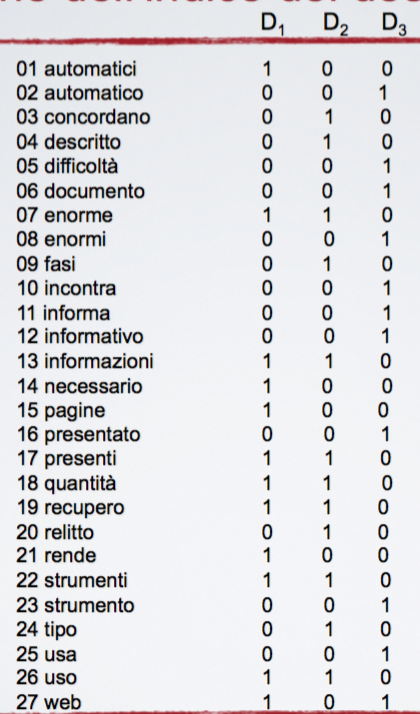
\includegraphics[width=0.7\linewidth]{images/l5-index-1}
  \caption{Indice delle parole}

\end{minipage}
\quad
\begin{minipage}[b]{0.45\linewidth}
	\centering
  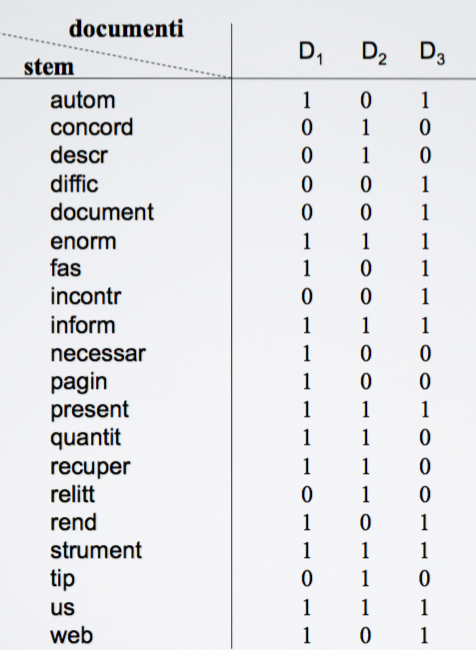
\includegraphics[width=0.7\linewidth]{images/l5-index-2}
  \caption{Indice degli stem. Ci sono dei casi in cui uno stem compare in tutti i documenti}
\end{minipage}
\end{figure}

Per risolvere questi problemi si posso utilizzare dei pesi per le varie parole, che vengono assegnati con una \textbf{funzione di pesatura} la quale può essere:

\begin{itemize}
	\item \textbf{Binaria}: se tiene conto solamente della presenza o meno della parola.
	\item \textbf{In base alla frequenza}: se considera il numero di occorrenze delle parole nei documenti e nella collezione.
\end{itemize}

\begin{figure}[htbp]
	\centering
	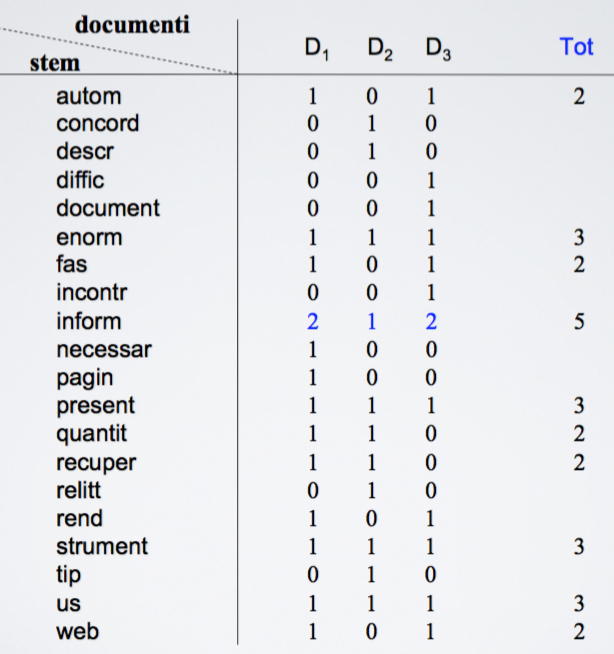
\includegraphics[width=0.4\linewidth]{images/l5-index-3}
	\caption{Indice degli stem che prende in considerazione anche le frequenze}
	\label{fig:l5-index-3}
\end{figure}


La pesatura può assegnare a ciascuno termine la frequenza di occorrenza del termine in un documento (\textbf{Term Frequency}) oppure la frequenza di occorrenza del termine all'interno della collezione (\textbf{Inverse Document Frequency}). Entrambi gli schemi verranno approfonditi più avanti.

Tipicamente nell'indice vengono memorizzati i dati grezzi, ovvero la frequenza assoluta, per calcolare i pesi in fase di reperimento, questo perché se l'indice contenesse direttamente i pesi, all'aggiunta di un nuovo documento sarebbe necessario andare a ricalcolare tutti i pesi di tutti i documenti. Un altro motivo è dato dal fatto che il peso serve solo per le parole che compaiono all'interno della query e quindi il calcolo non è oneroso e può essere fatto online.

L'indice finale dei descrittori è tipicamente una matrice sparsa molto grande e quindi è necessario utilizzare delle apposite strutture dati per memorizzare i dati.
Tipicamente viene utilizzato un \textbf{posting file} (o \textbf{inverted index}) che contiene la lista delle parole e per ogni parola è presente una lista di coppie, ognuna delle quali contiene l'identificativo del documento e la frequenza assoluta della parola all'interno del documento.

\begin{figure}[htbp]
	\centering
	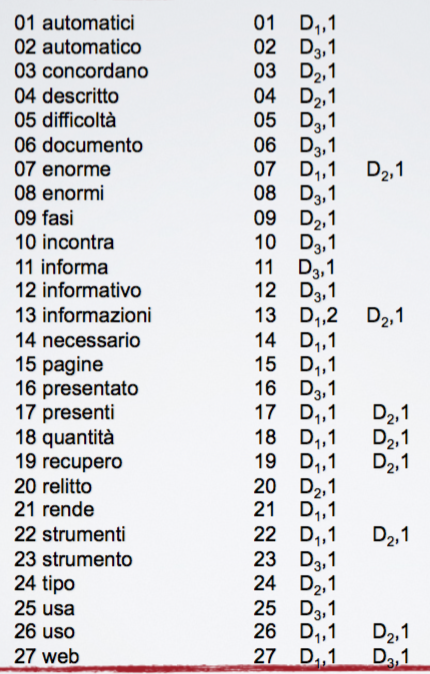
\includegraphics[width=0.3\linewidth]{images/l5-index-4}
	\caption{Esempio di posting file}
\end{figure}

\section{Ranking}

L'approccio base è quello di fornire una lista di documenti ordinata a partire dai dati presenti nell'indice.
Ma non sempre questo va bene:
\begin{itemize}
\item Due utenti possono effettuare la stessa query anche se hanno esigenze informative diverse.
\item Alcuni utenti filtrano la lista, non sempre si concentrano sul primo risultato, ma guardano anche altre cose, come lo snippet fornito nella SERP di Google.
\end{itemize}

Si può quindi pensare di creare un sistema di ranking che si basa su altre risorse, tipicamente sul machine learning, per creare un'ordinamento migliore e che tiene conto delle caratteristiche degli utenti.

Quindi l'idea è quella di fare un primo ranking tenendo conto degli indici del sistema e poi ristrutturarlo utilizzando altre tecniche.

% !TEX encoding = UTF-8
% !TEX TS-program = pdflatex
% !TEX root = computabilità e algoritmi.tex
% !TEX spellcheck = it-IT

\section{Predicati decidibili}\label{predicati-decidibili}

Nel mondo matematico spesso ci si chiede se valgono determinate
proprietà come:

$$ div(n,m) = \exists k : n \cdot k =m$$

La stessa cosa può essere vista come una relazione sui numeri naturali
$div \subseteq \mathbb{N} \times \mathbb{N}$. Tipicamente questo prende il nome di
\textbf{problema} o \textbf{predicato} e viene formalmente indicato con

$$Q(x_1, \ldots , x_k)$$

$$Q : \mathbb{N}^k \rightarrow \{vero,falso\} \: \text{oppure} \: Q \subseteq \mathbb{N}^k $$

Una volta formalizzato il predicato, ci si chiede se questo predicato è
\textbf{calcolabile} o \textbf{decidibile}

Un predicato $Q \subseteq \mathbb{N}^k$ si dice \textbf{decidibile} quando
$\mathcal{X}_A : \mathbb{N}^k \rightarrow \mathbb{N}$ è calcolabile, ovvero 

$$\mathcal{X}(\vec{x}) = \begin{cases}
1, \:& \text{ se } Q(\vec{x}) \\
0, \:& \text{altrimenti}
\end{cases} $$

Un predicato è decidibile quando la sua funzione $\mathcal{X}_Q$ è totale.

\subsection{Esempi di predicati decidibili}\label{esempi-di-predicati-decidibili}

\subsubsection{Uguaglianza}\label{uguaglianza}

Ad esempio $Q_1(x,y) = ``x=y''$ (uguaglianza) viene calcolato da

$$\mathcal{X}_{Q_1}(x,y) = \begin{cases}
1, \:& \text{se}\: x=y\\
0, \:& \text{altrimenti}
\end{cases}$$ 

Risulta triviale trovare un programma che calcola questa funzione

\begin{lstlisting}[language=URM]
J(1,2,SI)
Z(1)
J(1,1,FINE)
Z(1) #SI
S(1)
#FINE
\end{lstlisting}

\subsubsection{Pari e dispari}\label{pari-e-dispari}

Altro esempio $Q_2(x) = ``x \:\text{è pari}''$

\begin{lstlisting}[language=URM]
/*
    1: x
    2: 0, lo incremento per vedere se x è pari o meno
    3: 0, lo uso per tenere il codice compatto
*/
J(1,2,SI) #PARI?
S(2)
J(1,2,NO) #DISPARI?
S(2)
J(1,1,PARI?)
S(3) #SI
T(3,1) #NO
\end{lstlisting}

\subsubsection{Esercizio - Minore e uguale}\label{esercizio---minore-e-uguale}

$Q_3(x,y) = x \leq y$

\todo[inline]{todo}

\subsubsection{Esercizio - Divisibile}\label{esercizio---divisibile}

$Q_4(x,y) = div(x,y)$

\todo[inline]{todo}
\section{Computabilità su altri domini}\label{computabilituxe0-su-altri-domini}

Ci sono tanti modelli di calcolo che funzionano su svariati domini e noi
ci siamo concentrati solamente su quelli che utilizzano i numeri. 
Può però essere interessante vedere come cambiano le regole del gioco se viene
utilizzato un dominio diverso.

\textbf{Codifica effettiva}: Dato un dominio \emph{D}, si può trovare
una funzione $\alpha : D \rightarrow \mathbb{N}$ biunivoca e effettiva,
con inversa effettiva.

Alcuni domini che vanno bene sono $\mathbb{Z}, \mathbb{Q}, \mathbb{A}*$ ma non è possibile
utilizzare $\mathbb{R}$ perché non è numerabile.

Una volta fissato un dominio con una codifica effettiva, una funzione
$f: D \rightarrow D$ è \textbf{calcolabile} se $f^* = \alpha \circ f \circ \alpha^{-1}$ è URM-Calcolabile.

Ad esempio: $Q = \mathbb{Z},\: f : \mathbb{Z} \rightarrow \mathbb{Z},\: f(z) =
|z|$ è calcolabile perché è possibile trovare una funzione $\alpha : \mathbb{Z}
\rightarrow \mathbb{N}$ che codifica i numeri positivi con i numeri pari e
quelli negativi con i numeri dispari.

Così facendo viene stabilita una corrispondenza \textit{1-1} tra $\mathbb{Z}$ e $\mathbb{N}$.


$$\alpha(z) = \begin{cases}
2z\:& \text{se \textit{z} è positivo} \\
-2z-1\:& \text{se z è negativo}
\end{cases}$$

L'inversa viene definita come

$$\alpha^{-1}(n) = \begin{cases} \frac{n}{2} \:& \text{se \textit{n} è pari}\\
 \frac{-(n+1)}{2}\:& \text{se \textit{n} è dispari}\end{cases}$$

Pertanto $f^*$ risulta essere

\begin{align*}
	f^* &=\begin{cases}
	\alpha(f(\frac{n}{2})), \:\:\:& \text{se \textit{n} è pari}\\
	\alpha(f(\frac{-(n+1)}{2})), \:\:\:& \text{se \textit{n} è dispari}
	\end{cases} \\	
	f^* &= \begin{cases}
	n, \qquad\qquad\qquad\qquad& \text{se \textit{n} è pari} \\
	n+1, \qquad\qquad\qquad\qquad& \text{se \textit{n} è dispari}
	\end{cases} 
\end{align*}


\section{Composizione di funzioni calcolabili}\label{composizione-di-funzioni-calcolabili}

Si possono ottenere delle funzioni calcolabili utilizzando delle
composizioni di funzioni calcolabili più semplici.

La combinazione può essere fatta mediante:

\begin{itemize}
\item
  \textbf{Composizione funzionale}
\item
  \textbf{Ricorsione primitiva}, ovvero che termina sempre
\item
  \textbf{Minimizzazione illimitata}, ovvero l'iterazione fino a
  quando una certa condizione non viene soddisfatta.
\end{itemize}

In termini più tecnici, la classe $\mathcal{C}$ è \textbf{chiusa}
rispetto alle operazioni sopra riportate.

Ci si può spingere oltre, dimostrando che tutte le funzioni calcolabili
possono essere ottenute da combinazioni di funzioni calcolabili
elementari.

\textbf{Funzioni di base}: insieme delle funzioni calcolabili
elementari:

\begin{itemize}
\item
  $\underline{0} : \mathbb{N} \rightarrow \mathbb{N}^k,\: \underline{0}(x_1,\ldots{},x_k) = 0$
\item
  $succ: \mathbb{N} \rightarrow \mathbb{N},\: succ(x) = x+1$
\item
  $U_i^k : \mathbb{N}^k \rightarrow \mathbb{N},\: U_i^k(x_1,\ldots,x_k) = x_i$
\end{itemize}

e possono essere tutte calcolate da delle singole istruzioni URM.

\subsection{Notazioni e ipotesi per i programmi}\label{notazioni-e-ipotesi-per-i-programmi}

Per dimostrare la composizione di funzioni calcolabili viene fatta una
composizione dei programmi che le calcolano.

Per rendere le varie dimostrazioni più semplici si utilizzando varie
notazioni/ipotesi:

\begin{itemize}
\item
  Dato un programma \emph{P} in URM, $\rho(P) = max(\{i |  R_i \text{ è usato in }P\})$
\item
  \emph{P} è in forma standard, ovvero tutti i salti che fanno terminare
  il programma vanno a finire all'istruzione \emph{L(P) + 1}.
\item
  La concatenazione dei programmi viene indicata con \emph{P Q} e si
  assume che questa sia corretta rispetto ai salti a fine programma,
  ovvero che quando viene effettuata la concatenazione, le istruzioni di
  salto vengano aggiornate in modo opportuno.
\item
  Dato \emph{P}, $P[i_1,\ldots, i_k \rightarrow l]$ indica
  il programma che prende in input i registri $i_1\ldots, i_k$ e
  mette l'output in \emph{l} e non assume niente sugli altri registri,
  ovvero modifica \emph{P} in

\begin{lstlisting}[language=URM]
T(i1,1)
...
T(ik,k)
Z(k+1)
...
Z(rho(P))
P
T(1,l)
\end{lstlisting}

  C'è un piccolo problema con i vari trasferimenti \texttt{T(ij,j)} che
  possono sovrascrivere alcuni dati, pertanto è necessario stare attenti che
  questo non succeda utilizzando dei registri di supporto.
\end{itemize}

% !TEX encoding = UTF-8
% !TEX program = pdflatex
% !TEX root = MEMOC.tex
% !TEX spellcheck = it-IT

\chapter{Il metodo del simplesso e la dualità}

Inizialmente abbiamo visto come le soluzioni di un problema di programmazione lineare intera si trovino sui vertici della regione ammissibile e come fosse possibile trovare una soluzione in modo grafico.

Con il metodo del simplesso vengono fatte delle considerazioni simili, però a livello algebrico, in modo che possano essere generalizzate a casi che utilizzano più di due variabili.

\section{Le basi del simplesso}

La struttura generale di un modello è:

\begin{align*}
	\min(\max)\: &f(x) \\
		\st &g_i(x) = b_i \\
			&g_i(x) \leq b_i \\
			&g_i(x) \geq b_i \\
			&x \in \mathbb{R}^n
\end{align*}

\noindent dove $x$ è un vettore colonna di $n$ variabili reali, $f$ è la funzione obiettivo, $g_i$ sono le funzioni che rappresentano i vincoli (sono tutte funzioni $\mathbb{R}^n \to \mathbb{R}$) e i vari $b_i$ sono valori reali.

La cosa chiave è che i valori \textbf{sono numeri reali} e i vincoli sono \textbf{funzioni lineari}.

Si ha quindi che una \textbf{soluzione ammissibile} $x \in \mathbb{R}^n$ è un vettore che soddisfa tutti i vincoli, mentre la \textbf{regione ammissibile} è data dall'insieme delle soluzioni ammissibili e la soluzione ottima è una particolare soluzione ammissibile che minimizza (o massimizza) la funzione obiettivo.

Il processo di risoluzione consiste quindi nel determinare se:

\begin{itemize}
	\item Il problema è non ammissibile.
	\item Il problema è illimitato.
	\item Il problema ha una soluzione ottima.
\end{itemize}

\noindent La regione ammissibile può essere rappresentata come un \textbf{poliedro}, un'intersezione di un numero finito di semi-spazi chiusi e iperpiani in $\mathbb{R}^n$.

Un problema può quindi essere modellato come:

$$
\min (\max) \{c^T x : x \in P\}
$$

\noindent dove $P$ è un poliedro in $\Rn$.

\begin{figure}[htbp]
	\centering
	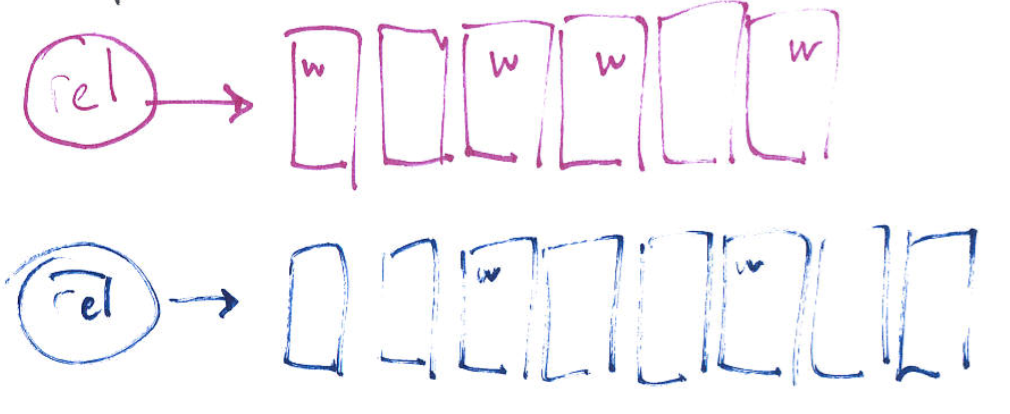
\includegraphics[width=0.6\textwidth]{images/l9-fig-1.png}
\end{figure}

\noindent Un \textbf{vertice} $v \in P$ è un vertice del poliedro $P$ se non è una \textbf{strict convex combination} di due punti distinti di $P$.

Un vertice $z \in \Rn$ è una \textbf{combinazione convessa} di due punti quando

$$
\exists \lambda \in [0,1] : z = \lambda x + (1-\lambda)y
$$

\noindent Viene detta \textbf{strict} se i valori 0 e 1 sono esclusi dall'intervallo.

Una \textbf{combinazione convessa} può essere fatta anche con più di due punti e può essere utilizzata per rappresentare una regione.
$z \in \Rn$ è una combinazione convessa di $x^1, x^2, \ldots, x^k$ se $\exists \lambda_1, \lambda_2, \ldots \lambda_k \geq 0$ tale che 

$$
\sum\limits_{i=1}^{k} \lambda_i = 1 \quad \text{e}\quad z = \sum\limits_{i=1}^{k} \lambda_ix^i
$$

\noindent Per il teorema di \textbf{Minkowski-Weyl}, la combinazione convessa di tutti i vertici di un poliedro permettono di rappresentare tutti i punti che appartengo al poliedro.

Quindi, per il \textbf{teorema del vertice ottimo}, se un problema LP ha può essere rappresentato da un poliedro $P$, allora esiste almeno una soluzione ottima e una di queste è su un vertice.

Questo è un risultato importante perché possiamo limitare la ricerca della soluzione ottima sui vertici di $P$ e non su tutto lo spazio.

\subsection{Rappresentazione algebrica dei vertici}

Considerando tutti i vincoli come delle uguaglianze abbiamo che i vertici del poliedro sono ottenuti intersecando tra loro le rette rappresentate dai vincoli (considerando il caso con due variabili).

Per trasformare i vincoli da disuguaglianze in uguaglianze è necessario aggiungere delle variabili di \textit{slack} che simulano il maggiore o minore.

Ad esempio:

	\begin{align*}
	3x_1 + 4x_2 &\leq 24 \\
	x_1 + 4x_2 &\leq 20 \\
	3x_1 + 2x_2 &\leq 18
	\end{align*}


\noindent diventa



	\begin{align*}
	3x_1 + 4x_2 +s_1&= 24 \\
	x_1 + 4x_2 +s_2&= 20 \\
	3x_1 + 2x_2 +s_3&= 18
	\end{align*}



Se si crea un sistema con queste nuove equazioni si ottengono due gradi di libertà, ovvero possiamo porre due variabili qualsiasi a zero per ottenere una soluzione unica.
Ad esempio se $s_1 = s_2=0$, otteniamo un sistema che può essere risolto e la cui soluzione rappresenta il vertice nel quale vengono imposti saturi il primo e secondo vincolo.

\subsection{Forma standard di un problema}

Per rendere l'approccio generico assumiamo che tutti i problemi sono scritti secondo la forma standard:

\begin{align*}
\min \: &c_1x_1+ c_2x_2 +\ldots + c_nx_n \\
\st &a_{i1}x_1 + a_{i2}x_2 +\ldots+a_{in}x_n = b_i \quad (i = 1 \ldots m) \\
&x_i \in \mathbb{R}_+ \quad (i = 1 \ldots n)
\end{align*}

\noindent Ovvero un problema in quale si minimizza sempre la funzione obiettivo, con tutte le variabili $\geq 0$ (per rendere semplice identificare le soluzioni non ammissibili), con tutti i vincoli che sono uguaglianze e con tutte le parti destre $b_i$ dei vincoli $\geq 0$.

Si può sempre trasformare un problema generico in forma standard.

\begin{itemize}
	\item Se il problema iniziale è una massimizzazione, basta passare alla minimizzazione e moltiplicare la funzione obiettivo per $-1$.
	\item Se ci sono delle variabili negative è possibile sostituirle con un'altra variabile che è positiva, es $x_+ = - x_\text{-}$.
	\item Se ci sono delle disuguaglianze è possibile aggiungere le variabili slack.
	\item Se un $b_i$ è negativo si può moltiplicare tutto il vincolo per $-1$. 
\end{itemize}

\section{Il metodo del simplesso}

\noindent Assumiamo che il problema sia modellato dal sistema $Ax = b$, $A \in \R^{m\times n}, \rho(A) = m, m <n$.
Definiamo come \textbf{base di $A$} una sotto-matrice quadrata $B \in \R^{m \times m }$ tale che abbia rango massimo, ottenuta prendendo $n$ colonne linearmente indipendenti della matrice $A$. 

Abbiamo quindi che $A = [B|N]$ con $det(B) \neq 0$ e $x = \begin{bmatrix}
x_B\\ 
x_F
\end{bmatrix}$ con $x_B \in \R^m$ e $x_F \in \R^{n-m}$.

Così facendo possiamo riscrivere il sistema come 

\begin{align}
Ax &= b \\
[B|F]\begin{bmatrix}
x_B\\ 
x_F
\end{bmatrix} &= b\\
B x_B + F x_F &= b
\end{align}

\noindent Posso quindi ricavare i valori di $x_B$, ovvero delle variabili presenti nella base con

$$
x_B = B^{-1}b - B^{-1}F x_F
$$

\noindent Ponendo le variabili $x$ fuori base ($x_F$) uguali a 0, otteniamo una \textbf{soluzione base}.
Il nome \textbf{base} deriva dal fatto che l'insieme dei vettori che compongono la base sono tutti linearmente indipendenti.

Quindi in una soluzione base abbiamo almeno $n-m$ variabili uguali a 0 (se ce ne sono di più la base diventa degenere).

Tornando al nostro problema di partenza abbiamo che una soluzione base diventa \textbf{ammissibile} quando soddisfa tutti i vincoli di partenza, ovvero

$$
x_B = B^{-1}b \geq 0
$$

\noindent Inoltre, per la proprietà di \textbf{corrispondenza tra vertici e soluzioni di base} si ha che se $x$ è una soluzione di base, allora
\begin{equation}
Ax = b \Leftrightarrow x \text{ è vertice di }P 
\end{equation} 
 
Per ottenere delle basi diverse, e quindi cercare un altro vertice, basta cambiare quali variabili sono fissate a 0.

Combinando ciò con il teorema del vertice ottimo si ottiene il \textbf{Teorema fondamentale delle programmazione lineare}, il quale asserisce che se esiste una soluzione ottima allora esiste anche una soluzione di base ammissibile e ottima.

Da qui nasce l'idea del metodo del simplesso, il quale parte da un problema posto in forma standard e da una soluzione ammissibile per trovare un vertice ottimo.

\subsection{I passi dell'algoritmo}

L'algoritmo del simplesso considera un problema in forma standard e necessita di una soluzione ammissibile di base di partenza.
L'algoritmo passa iterativamente da una soluzione ammissibile di base ad una adiacente che permetta di migliorare il valore corrente della funzione obiettivo fino al raggiungimento dell'ottimo.

\subsection{Passo -1: Passaggio alla forma standard}

Trasformo il problema nella forma

\begin{align*}
\min \:& z=c^Tx \\
\st& Ax=b \\
&x\geq 0
\end{align*}

\subsection{Passo 0: Base iniziale e tableau}

Fisso una base iniziale di partenza e riscrivono il problema in modo che:

\begin{itemize}
\item Nei vincoli, le variabili di base siano espresse solamente nei termini delle variabili fuori base.
\item La funzione obiettivo contenga solo variabili non di base
\end{itemize}

\noindent ovvero il problema diventa:

\begin{align*}
\min \: z=\: &c_{B}^T B^{-1}b + (c_{F}^T - c_{B}^T B^{-1}F)x_F \\
\st& Ix_B + B^{-1}Fx_F = B^{-1}b \\
&x\geq 0
\end{align*}

\noindent che può essere sintetizzato in 

\begin{align*}
\min \: z=\: &z_B + \overline{c}_{F}^Tx_F \\
\st& Ix_B + \overline{F}x_F = \overline{b} \\
&x\geq 0
\end{align*}

\noindent dove:

\begin{itemize}
\item $ \overline{b} =  B^{-1}b $ rappresenta il valore delle variabili di base nella soluzione corrente.
\item $ z_B =  c_{B}^T B^{-1}b$ è il valore corrente della funzione obiettivo.
\item $ \overline{F} = B^{-1}F $ sono le colonne delle variabili fuori base espresse nei termini della base corrente.
\item $ \overline{c}_{F}^T = c_{F}^T - c_{B}^T B^{-1}F$ sono i costi ridotti per le variabili fuori base.
\end{itemize}

Questa forma prende il nome di \textbf{forma tableau} o forma canonica.

\begin{table}[htbp]
\centering
\begin{tabular}{c|c|c|c|}
\cline{2-4}
$-z$ & $-z_B$           & $0$     & $\overline{c}_{F}^T$ \\ \cline{2-4} 
   & $\overline{b}$ & $Ix_B$ & $\overline{F}x_F$         \\ \cline{2-4} 
\end{tabular}
\end{table}

\begin{figure}[htbp]
	\centering
	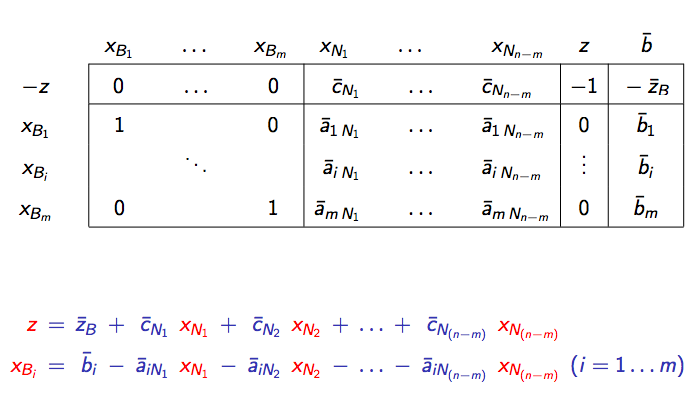
\includegraphics[width = .7\textwidth]{images/l9-fig-3.png}
	\caption{Il talbeau del simplesso}
\end{figure}

\subsection{Passo 1: Scelta della variabile da fare entrare in base}

L'operazione di cambio base permette di passare da una soluzione ammissibile di base ad una adiacente.

Considerando l'espressione della funzione obiettivo in termini di variabili fuori base, ovvero considerando la prima riga del tableau, abbiamo che:

\begin{align*}
z &= z_B + \overline{C}_{F}^Tx_F \\
&= z_B + \overline{C}_{F_1}^Tx_{F_1} + \ldots + \overline{C}_{F_n}^Tx_{F_n}
\end{align*}

Se entra in base una nuova variabile $x_{F_j}$, ovvero diventa diversa da 0, si ha che il nuovo valore della funzione obiettivo diventerà

$$
z = z_B + \overline{C}_{F_j}^Tx_{F_j}
$$

dove $\overline{C}_{F_j}$ rappresenta l'incremento marginale della funzione obiettivo all'aumentare di $x_{F_j}$ e viene detto costo ridotto. 

\subsection{Passo 2: Scelta della variabile uscente}

La nuova variabile che entra in base deve assumere il massimo valore possibile che non rende inammissibile la soluzione.
Pertanto viene assegnato alla variabile entrante $x_j$ il valore $\vartheta$ che preserva l'ammissibilità della soluzione, ovvero non rende le altre variabili negative.

Il valore $\vartheta$ viene scelto con la \textbf{regola del quoziente}

$$
\vartheta = \min\limits_{i | \overline{a}_{ij} > 0} \bigg\{ \frac{\overline{b}_i}{\overline{a}_{ij}} \bigg\}
$$

dove $\overline{a}_{ij}$ è il coefficiente di $x_j$ nel vincolo $i$.

La variabile uscente è quindi quella che corrisponde al minimo quoziente, ovvero a quella che viene azzerata ponendo $x_j = \vartheta$.

Da notare che se tutti gli $\overline{a}_{ij}$ sono $\leq 0$, il problema è illimitato, perché la variabile $x_j$ può entrare in base con un valore qualsiasi, migliorando sempre la funzione obiettivo.

\subsection{Passo 3: Cambio di base} 

Se $x_j$ è la variabile selezionata per entrare in base e $x_k$ è la variabile uscente è necessario effettuare un'operazione di pivot della matrice in modo che la colonna corrispondente a $x_j$ diventi della forma $ \begin{bmatrix}
0\\ 
e_k
\end{bmatrix} $ dove $e_j$ è un vettore di 0 con l'elemento di indice $j = 1$.

\subsection{Passo 4: Condizione di terminazione}

Il metodo del simplesso continua fino a che non ci sono più costi ridotti negativi e pertanto la soluzione di base è anche ottima.

Bisogna però stare attenti a non visitare sempre la stessa sequenza di vertici. Per evitare ciò è possibile scegliere di far entrare in base sempre la variabile di indice minimo tra tutte quelle che hanno costi ridotti negativi.



\subsection{Algoritmo del simplesso nel dettaglio}

\begin{enumerate}
	\item Trasforma il PL in forma standard e trova una base iniziale feasible $B$. La base può essere trovata risolvendo un problema artificiale.
	\item Ripeti finché non trovi una soluzione ottima o non ti accorgi che il problema è illimitato:
	\begin{itemize}
		\item Poni il problema in forma canonica rispetto la base $B$
		\begin{align*}
		z &= \overline{z}_B + \overline{c}_{F_1} x_{F_1} 
		+ \overline{c}_{F_2} x_{F_2} + \ldots + \overline{c}_{F_{n-m}} x_{F_{n-m}} \\
		x_{B_i} &= \overline{b}_i - \overline{a}_{iF_1} x_{F_1} - \overline{a}_{iF_2} x_{F_2} - \ldots - \overline{a}_{iF_{n-m}} x_{F_{n-m}} \qquad \forall \: i \in [1 \ldots m]
		\end{align*}
		\item Se $\overleftarrow{c}_j \geq 0 \forall \ j$, la base $B$ è ottima. Fermati.
		\item Se $\exists h : \overline{c}_h < 0 , \overline{a}_{ih}\leq 0 \ \forall i$, il problema è illimitato. Fermati.
		\item Scegli una variabile $x_h$ da portare in base tra tutte quelle con costi ridotti negativi.
		\item Trova la variabile $x_{B_t}$ con $ t = \arg \min_{i = 1 \ldots m} \bigg\{ \frac{\overline{b}_i}{\overline{a}_{ih}}  : \overline{a}_{ih} > 0 \bigg\}$
		\item $B \leftarrow B \oplus A_h \ominus A_{B_t}$, ovvero effettua il cambio di base.
	\end{itemize}
\end{enumerate}

Da notare che tutti i vari passaggi possono essere replicati utilizzando i calcoli matriciali al posto del tableau del simplesso.


\subsection{Metodo delle due fasi}

Questo metodo permette di trovare una soluzione ammissibile di partenza per il metodo del simplesso.

Dato un problema in forma standard

\begin{align*}
\min \:& z=c^Tx \\
\st& Ax=b \\
&x\geq 0
\end{align*}

\noindent viene creato un problema artificiale, aggiungendo al problema di partenza un nuovo vettore di variabili $y \in \R^{m}$ e cambiando la funzione obiettivo:

\begin{align*}
w^* = \min \:& w= I^Ty = y_1 + y_2 + \ldots + y_m \\
\st& Ax + Iy=b \\
&x, y\geq 0
\end{align*}

Per come è formulato questo problema ho già che $Iy$ è una base ammissibile ma non ancora espressa in forma canonica.
Inoltre, questo problema è sempre ammissibile, perché la soluzione $x = 0, y=b$ è ammissibile ed inoltre non è mai illimitato perché la funzione obiettivo è la minimizzazione di una sommatoria con termini tutti maggiori di 0, pertanto l'ottimo è 0.

Una volta messo in forma canonica il problema artificiale, posso risolverlo utilizzando il simplesso ottenendo un valore ottimo $w*$, che può essere:

\begin{itemize}
\item $w^* > 0$: il problema originale non è ammissibile e quindi non ha senso passare alla fase 2.
\item $w^* = 0$: in questo caso tutte le variabili artificiali sono necessariamente nulle e quindi possono essere tolte dai vincoli, rendendoli comunque soddisfatti, pertanto il problema di partenza è ammissibile. Se tutte le $y$ sono fuori base, allora il tableau finale può essere usato come tableau di partenza per il simplesso sul problema originale, altrimenti è necessario effettuare un cambio di base in modo da togliere dalla base tutte le $y$.


\end{itemize}

















% !TEX encoding = UTF-8
% !TEX program = pdflatex
% !TEX root = InformationRetrieval.tex
% !TEX spellcheck = it-IT

% 10 Novembre 2016
%\section{Modello probabilistico}
%\subsection{Basi di probabilità}
%\subsubsection{Interpretazione grafica del costo degli errori}

\chapter{Sistemi di reperimento dell'informazione}

In questa parte parleremo dei sistemi di reperimento che sono disponibili su internet e che sono pronti all'uso.

\section{Sistemi open-source}

I 3 principali sistemi di IR disponibili sul mercato open-source sono:

\begin{itemize}
	\item \textbf{Apache Lucene}: viene tipicamente utilizzato all'interno di \textbf{Apache Solr}, una soluzione che permette di creare dei motori di ricerca ad-hoc per l'ambito enterprise.
	\item \textbf{Terrier}: progetto accademico che raramente viene utilizzato a livello commerciale.
	\item \textbf{Indri}: sistema orientato verso modelli di reperimento che utilizzano language modelling (cose avanzate che probabilmente non affronteremo).
\end{itemize}

\noindent Tutti questi sistemi permettono di:

\begin{itemize}
	\item Indicizzare collezioni di documenti, con analisi lessicale, stop-list, stemmer e creazione di indice.
	\item Indicizzare ed elaborare le query.
	\item Reperire documenti producendo delle liste ordinate in base alla rilevanza (ranking).
	\item Utilizzare diversi modelli di reperimento: booelano, vettoriale, probabilistico.
\end{itemize}

\noindent Tutti questi sistemi sono pensati per gestire la lingua inglese, ma permettono comunque di utilizzare altre lingue.


\subsection{Apache Lucene}

Sistema open-source dell'Apache Software Foundation, creato del 1999, tipicamente utilizzato all'interno di sistemi commerciali.

\subsection{Terrier}

Sviluppato dal gruppo di ricerca dell'Università di Glasgow a partire dal 2001.

L'implementazione del sistema è quello che è, perché viene sviluppato a pezzi da vari studenti e ricercatori.

L'utilizzo tipico di questo sistema è in ambito accademico o nel mondo della ricerca.

Prevede dei modelli di \textit{learning to rank}, ovvero modelli che apprendono come fare ranking guardando come altri modelli hanno fatto ranking per la stessa query. 

\subsection{Indri}

Sempre sviluppato da un'università, scritto in C++ e tipicamente utilizzato in ambiti di ricerca.

Viene utilizzata con la libreria RankLib e  implementa vari algoritmi di \textit{learning to rank}.

\section{Funzionamento di Terrier}

Per utilizzarlo è necessario scaricare l'installer dal sito \url{http://www.terrier.org}.

Dopo l'installazione, che alla fine è la decompressione di un pacchetto, vengono create un po' di cartelle. Quelle più interessanti sono:

\begin{itemize}
	\item \texttt{bin}: contiene gli script e i file eseguibili.
	\item \texttt{etc}: contiene i file di configurazione \texttt{terrier.properties} e \texttt{collection.spec}
	\item \texttt{target/lib}: contiene i file jar, tra cui quelli di Terrier. Qui va messa la nostra versione di Terrier modificata.
	\item \texttt{var}: contiene l'indice e i file dei risultati.
\end{itemize}


\subsection{Properties}

Il file con tutta la configurazione di sistema si trova su \texttt{etc/terrier}.
In questo file è possibile specificare quali file indicizzare, quale tokenizer utilizzare, stop-list, stemmer, ecc.

\subsection{Documentazione}

Nel sito web si trova la documentazione completa del sistema, non solo la JavaDoc, ma anche la descrizione del funzionamento di Terrier, con anche degli esempi di utilizzo.

\section{Indicizzazione con Terrier}

\begin{figure}[htbp]
	\centering
	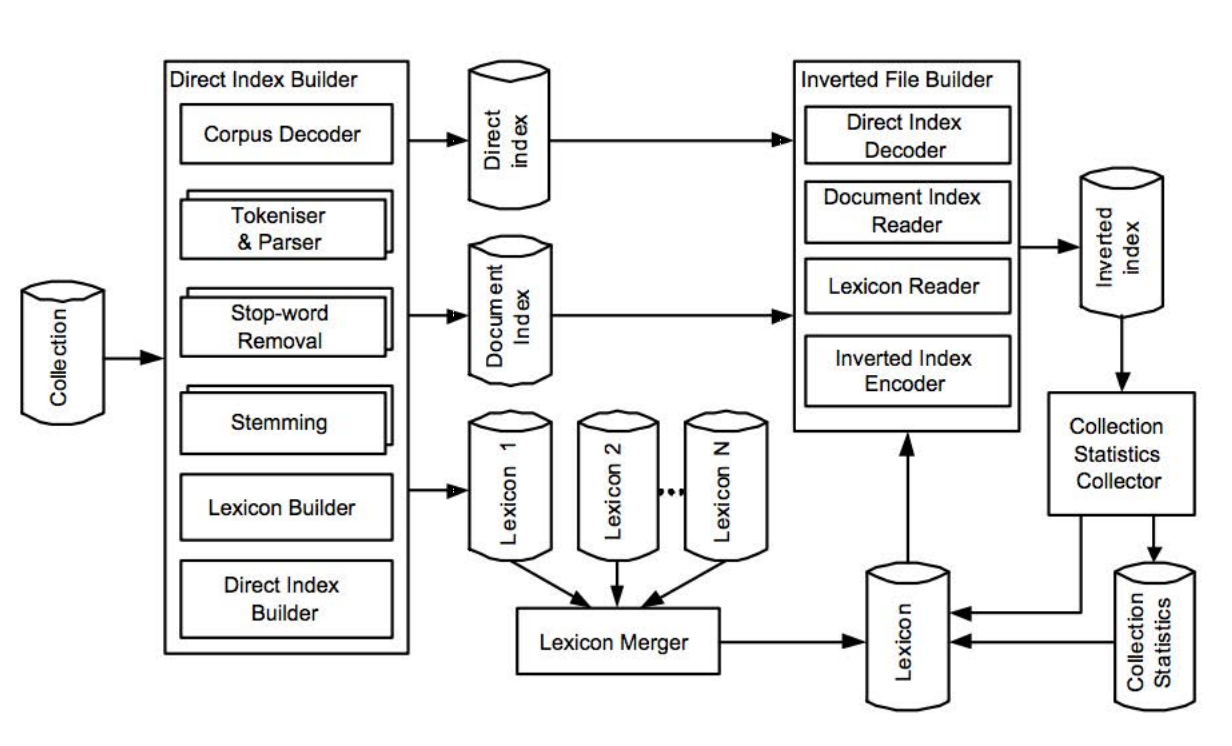
\includegraphics[width=0.9\linewidth]{images/l12-fig-1.png}
\end{figure}

Si parte da una collezione di documenti (corpus), sulla quale viene costruito l'indice diretto, con le fasi viste precedentemente.
La costruzione del lexicon (dizionario) viene fatta prima costruendo \textit{N} dizionari per i vari documenti, che poi vengono uniti in modo automatico. Il dizionario generato contiene delle statistiche relative al \textit{tf} e \textit{idf}.

Viene poi creato l'indice inverso che contiene un po' di informazioni relative ai termini. Tipicamente è presente tutto quello che serve, ma può capitare che sia necessario modificare la creazione dell'indice per avere a disposizione informazioni extra, utili ai modelli di reperimento.

\subsection{Un esempio di indicizzazione}

Supponiamo di voler indicizzare i file presenti all'url \url{http://www.dei.unipd.it/~silvello/IR2016-2017/small_test_collections/text/} e che siano presenti in locale nel percorso \texttt{/IR2016-2017/collections/text/}.

Il primo passo è andare a specificare all'interno del file \texttt{etc/collection.spec} quali file indicizzare, indicandone il percorso assoluto.
Si può fare a mano, oppure si può fare in modo automatico utilizzando uno script bash:

\begin{center}
	\texttt{\$ sh bin/trec\_setup.sh /path-to-collection/}
\end{center}

\noindent Serve poi ri-configurare il file di properties, perché ad ogni esecuzione di \texttt{trec\_steup} viene inizializzato.

\begin{lstlisting}
#default controls for query expansion
querying.postprocesses.order=QueryExpansion
querying.postprocesses.controls=qe:QueryExpansion
#default controls for the web-based interface. SimpleDecorate
#is the simplest metadata decorator. For more control, see Decorate.
querying.postfilters.order=SimpleDecorate,SiteFilter,Scope
querying.postfilters.controls=decorate:SimpleDecorate,site:SiteFilter,scope:Scope

#default and allowed controls
querying.default.controls=
querying.allowed.controls=scope,qe,qemodel,start,end,site,scope

#document tags specification
#for processing the contents of
#the documents, ignoring DOCHDR
TrecDocTags.doctag=DOC
TrecDocTags.idtag=DOCNO
TrecDocTags.skip=DOCHDR
#set to true if the tags can be of various case
TrecDocTags.casesensitive=false

#query tags specification
TrecQueryTags.doctag=TOP
TrecQueryTags.idtag=NUM
TrecQueryTags.process=TOP,NUM,TITLE
TrecQueryTags.skip=DESC,NARR

#stop-words file
stopwords.filename=stopword-list.txt

#the processing stages a term goes through
termpipelines=Stopwords,PorterStemmer
\end{lstlisting}

\noindent Il primo blocco (1-11) riguarda le funzionalità di query expansion e la possibilità di utilizzare Terrier come applicazione web. A noi questa cosa non ci interessa.

Il secondo blocco (13-26) riguarda le proprietà per la valutazione sperimentale di un sistema IR. Servono per specificare quali tag devono essere indicizzati\footnote{Nel caso di documenti strutturati}. Il tutto sarà più chiaro dopo aver fatto la parte di valutazione.

Il terzo blocco (28-32) contiene il percorso per raggiungere il file contenente le stop-word e la configurazione della pipeline di indicizzazione dei termini.
Per usare il nostro stemmer dovremmo specificare un \texttt{LookupStemmer}, mentre per ottenere l'indice puro dei termini è necessario lasciare il campo vuoto.

\begin{figure}[htbp]
	\centering
	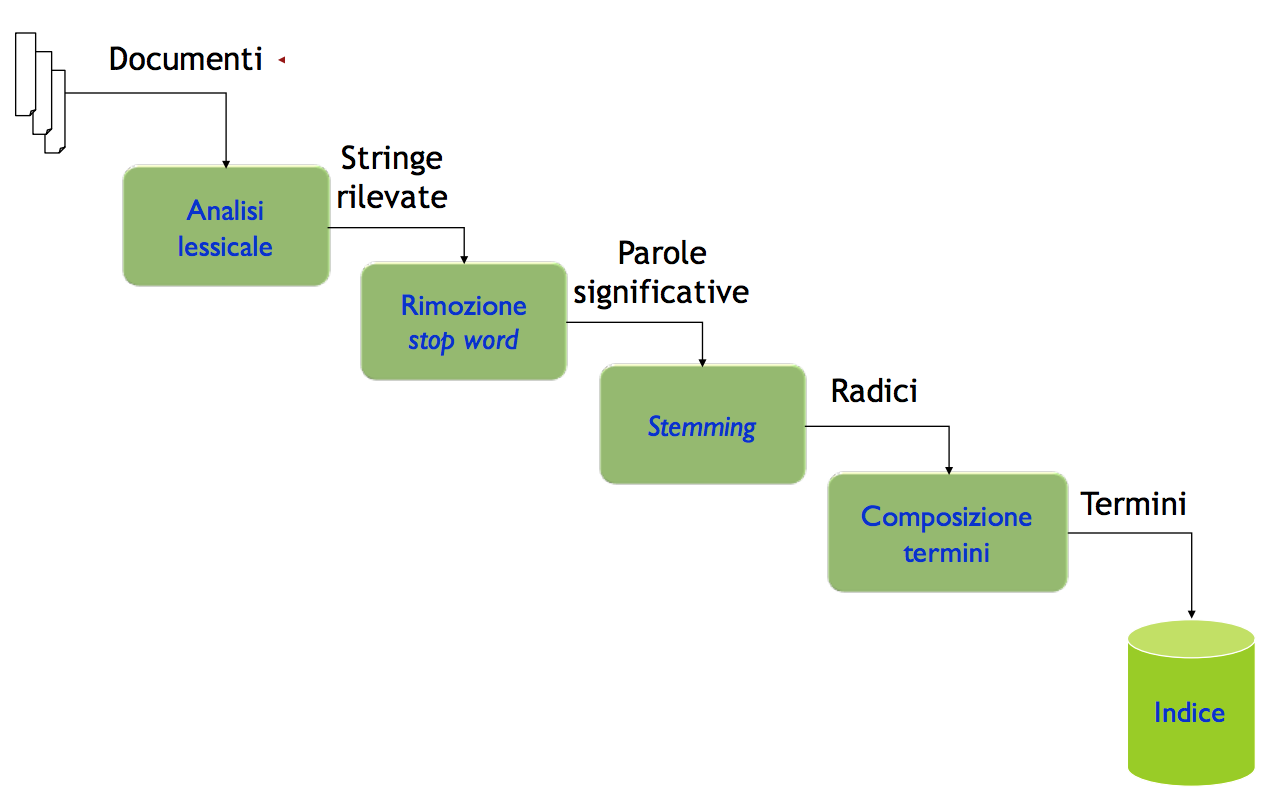
\includegraphics[width=0.7\linewidth]{images/l12-fig-3.png}
\end{figure}

\noindent Le varie proprietà del file properties influiscono sulla fase di analisi lessicale nel seguente modo:

\begin{itemize}
	\item \textbf{Documenti}: specificati nel file \texttt{collection.spec}
	\item \textbf{Analisi lessicale}:
	\begin{itemize}
		\item \texttt{tokeniser=EnglishTokeniser}: che tokenizer utilizzare, dipende dalla lingua dei documenti.
		\item \texttt{trec.encoding=UTF-8}: codifica dei caratteri, noi utilizziamo UTF-8 perché dobbiamo gestire anche le lettere accentate e i caratteri in cirillico. Utilizzare UTF-16 è un over-kill, può essere utile con le lingue giapponesi.
		\item \texttt{trec.collecion.class=SimpleFileCollection} e \texttt{trec.document.class=FileDocument}: specificano le classi Java da utilizzare per fare la tokenizzazione (analisi lessicale). In questo caso \texttt{SimpleFileDocument} permette di indicizzare file di testo, mentre per utilizzare documenti strutturati serve un'altra classe.
	\end{itemize}
	\item \textbf{Rimozione stop-word}:
	\begin{itemize}
		\item \texttt{stopwords.filename=stopword.txt}: file con le stop-word.
		\item \texttt{termpipelines=Stopwords}: aggiunge nella pipeline la rimozione delle stop-word.
	\end{itemize}
	\item \textbf{Stemming}: \texttt{termpipelines=PorterStemmer} per la selezione dello stemmer da utilizzare.
	\item \textbf{Composizione termini}: niente.
	\item \textbf{Indice}:
	\begin{itemize}
		\item \texttt{index.meta.forward.keys=filename}: codice per riferirsi ai documenti indicizzati. Con questa impostazione viene utilizzato il nome del file.
		\item \texttt{index.meta.forward.keylens=512}: dimensione della chiave.
	\end{itemize}
\end{itemize}

\noindent Per avviare l'indicizzazione viene utilizzato lo script:

\begin{center}
	\texttt{\$ sh bin/trec\_terrier.sh -i}
\end{center}

\noindent L'indice così prodotto viene messo nella cartella \texttt{var/index}, ma può essere modificata dal file properties.

Dopo aver creato l'indice è possibile ri-eseguire il comando di creazione dell'indice per ricavare alcune informazioni dall'indice, passandogli uno dei seguenti flag:

\begin{itemize}
	\item \texttt{- -printlexicon} contenuto del ``lexicon''
	\item \texttt{- -printinverted} contenuto dell'``inverted file''
	\item \texttt{- -printdirect} contenuto del ``direct file''
	\item \texttt{- -printstats} statistiche
	\item \texttt{- -printmeta} the meta structure
\end{itemize}

\noindent Una possibile riga del lexion prodotto è

\begin{center}
	\textit{direct,term55 Nt=5 TF=8 \@{0 122 2}}
\end{center}

\noindent La prima cosa è il termine stemmato, il secondo è l'identificatore progressivo, c'è poi il numero di documenti contenti il termine (\textit{Nt}) e la term frequency \textbf{nella collezione}. L'ultima parte è un'informazione interna di Terrier.

Nell'indice trasposto le informazioni sono memorizzate con un'identificativo interno del documento.
Una riga dell'indice trasposto è:

\begin{center}
	\textit{513 (0,2) (1,1) (3,2)}
\end{center}

\noindent Dove il primo campo è l'identificativo del termine, mentre le coppie contengono l'identificativo del documento e la \textit{TF} del termine all'interno del documento.
Da notare che il l'identificativo del termine (\textit{es: 513}) non viene inserito all'interno del lexicon, è necessario fare affidamento al numero di riga.

\section{Indicizzazione e interrogazione di documenti non in inglese}

La collezione di riferimento è adesso in italiano ed in formato pdf. Può essere recuperata all'url \texttt{www.dei.unipd.it/~silvello/IR2016-2017/small\_test\_collections/pdf/}.

Le modifiche da fare riguardano:

\begin{itemize}
	\item \texttt{tokeniser=UTFTokeniser}: perché ci sono gli accenti. Stranamente utilizzare questo tokeniser con l'inglese da dei problemi.
	\item \texttt{trec.document.class=PDFDocument}: perché stiamo utilizzando dei pdf.
	\item \texttt{stopwords.filename=.../italian\_stoplist.txt}: perché servono le stop-words specifiche per la lingua.
	\item \texttt{termpipelines=ItalianSnowballStemmer}: un altro stemmer interno di Terrier creato per la lingua italiana. Nel nostro progetto abbiamo uno stemmer statistico e quindi non dovremmo andare a cambiare questo parametro quando cambiamo lingua.
\end{itemize}

\section{Configurazione di Terrier per il nostro progetto}

Una volta creato lo stemmer statistico, per farlo utilizzare a Terrier dobbiamo specificare le seguenti proprietà:

\begin{lstlisting}
termpipeline=LookupStemmer
lookupstemmer.filename=<pathToFile> // verso il file prodotto dal nostro script
lookupstemmer.encoding=UTF-8
tokeniser=UTFTokeniser
\end{lstlisting}

\noindent Per generare il dizionario completo delle parole non dobbiamo specificare lo stemmer.

Per il progetto non è richiesto l'uso di stop-list, ma se si vogliono fare dei test extra è possibile utilizzarle.




% !TEX encoding = UTF-8
% !TEX TS-program = pdflatex
% !TEX root = apprendimento_automatico.tex
% !TEX spellcheck = it-IT

\section{Lezione 16 - Naive Bayes}

Questa tipologia di classificatore risulta essere una delle tecniche più semplici e popolari, che in alcuni casi fornisce delle prestazioni simili a quello offerte dalle reti neurali e SVM.

Conviene utilizzare questo classificatore quando:

\begin{itemize}
	\item Si ha a disposizione un elevato numero di dati;
	\item Gli attributi che descrivono le istanze sono condizionalmente indipendenti data la classificazione.
\end{itemize}

Il caso d'uso più famoso per questo classificatore è la categorizzazione di documenti testuali basata sulla frequenza delle parole.

\subsection{Funzionamento del classificatore}

Si ha a disposizione un training set composto da $(x_i, y_i)$, dove $x_i$ sono le istanze sulle quali fare apprendimento e $y_i$ è l'etichetta dell'istanza.

Ogni istanza $x_i$ è descritta da una tupla di attributi $<a_1, \ldots, a_n$ e le possibili etichette $y_i$ sono dei valori $v_j \in V$.

La funzione che si vuole apprendere è quindi $f :  X \rightarrow V $ e questo viene fatto ritornando l'etichetta più probabile:

$$
v_{MAP} = argmax_{v_j in V} P(v_j | a_1 , \ldots, a_n)
$$ 

ovvero l'etichetta che ha probabilità a posteriori maggiore data la descrizione dell'esempio.

Utilizzando la regola di Bayes si ottiene:

\begin{align*}
v_{MAP}  &= argmax_{v_j in V}\frac{ P( a_1 , \ldots, a_n | v_j)P(v_j)}{P( a_1 , \ldots, a_n)} \\
				&= argmax_{v_j in V} P( a_1 , \ldots, a_n | v_j)P(v_j)
\end{align*}

Il classificatore Naive Bayes assume che i valori degli attributi di una determinata istanza sono tra loro condizionalmente indipendenti data la classificazione, ovvero

$$
P(a_1,\ldots, a_n | v_j) = \prod_i P(a_i | v_j)
$$

con questa ipotesi il classificatore naive di Bayes diventa:

$$ 
v_{NB} = argmax_{v_j \in V} P(v_j)\prod_i P(a_i | v_j)
$$

\subsection{Apprendimento del classificatore}

L'apprendimento del classificatore consiste nello stimare i valori per $P(v_j)$ e $P(a_i | v_j)$ ed è possibile farlo andando a contare le occorrenze all'interno del training set.

\begin{enumerate}
	\item Per ogni valore target $v_j$:
		\begin{enumerate}
			\item $\hat{P}(v_j) \leftarrow$ stima di $P(v_j)$
			\item Per ogni valore $c_k$ di ogni attributo $a_i$:
				\begin{enumerate}
					\item $\hat{P}(c_k | v_j) \leftarrow$ stima di $P(c_k | v_j)$
				\end{enumerate}
		\end{enumerate}
\end{enumerate}

La classificazione viene poi effettuata usando le probabilità stimate.

Rispetto agli altri algoritmi di apprendimento finora visti, non viene effettuata una ricerca nello spazio delle ipotesi, ma viene costruita stimando le probabilità delle varie etichette.


\subsection{Considerazioni aggiuntive}

L'assunzione dell'indipendenza condizionale utilizzata dal Naive Bayes non sempre viene rispettata, tuttavia questo non influisce sulle prestazioni del classificatore.

Oltretutto, le stime effettuate utilizzando il training set non è necessario che siano precise, basta che valga la relazione:

$$ 
argmax_{v_j \in V} \hat{P}(v_j)\prod_i \hat{P}(a_i | v_j) = argmax_{v_j \in V} P(v_j)\prod_i P(a_i | v_j)
$$

Durante la stima delle probabilità può succedere che nessun esempio del training set sia classificato con l'etichetta $v_j$ ed abbia l'attributo $a_i = c$.
Se questo succede, la probabilità a posteriori stimata risulta essere 0 e la classificazione $v_j$ risulterà essere sempre improbabile.

$$ \hat{P}(c | v_j) = 0 \text{ e } \hat{P}(v_j)\prod_i \hat{P}(a_i | v_j) = 0$$

Una soluzione tipica è quella di andare a prendere in considerazioni degli \textbf{esempi virtuali} che non compaiono nel training set, ovvero:

$$
\hat{P}(c | v_j) = \frac{n_k + mp}{n +m}
$$

dove:

\begin{itemize}
	\item $n$ è il numero di esempi di apprendimento con $v = v_j$;
	\item $n_k$ è il numero di esempi di apprendimento con $v = v_j \text{ e } a_i = c$;
	\item $m$ è il numero di esempi virtuali, detto anche \textbf{equivalent sample size};
	\item $p$ è una stima per la probabilità $\hat{P}(c | v_j)$ nota a priori, che può essere influenza da delle conoscenze sul dominio oppure può essere uniforme per tutti i possibili valori dell'attributo.
\end{itemize}










% !TEX encoding = UTF-8
% !TEX program = pdflatex
% !TEX root = InformationRetrieval.tex
% !TEX spellcheck = it-IT

\chapter{Web search}

La principale differenza tra i documenti puramente testuali e quelli web è che la collezione di documenti non è nota a priori.
Inoltre, per i file testuali, avevamo un identificativo univoco per ciascun documento e ogni volta che andavamo a fare reperimento, fornivamo in risposta dei documenti diversi, mentre nell'ambito web possono esserci due pagine con lo stesso contenuto.
In più le pagine web sono costruite con dei linguaggi di mark-up che forniscono delle informazioni che permetto di costruire degli \textbf{authority file} per distinguere quali pagine sono state create da delle persone autorevoli.
Un'ulteriore differenza sta nel fatto che i documenti web possono essere tra loro linkati, cosa che non avviene per i documenti testuali.

\section{Il contesto Web}

La collezione di documenti è costituita da una collezione di pagine web che possono essere o documenti HTML o documenti multimediali (PDF, JPEG, MP3, ecc.).

Per quanto riguarda le pagine web si possono sfruttare gli hyperlink per ottenere informazioni aggiuntive relative ai documenti.
Questi hyperlink possono essere sfruttati dai \textbf{web crawler}, programmi che navigano sul web per indicizzare le pagine.
L'esecuzione di questi programmi deve essere continua, perché il web è un ambiente dinamico e anche il contenuto delle pagine già indicizzate può cambiare.

Inoltre le pagine web sono composte da un header che contiene dei meta-tag che, se usati correttamente, descrivono il contenuto della pagina web, fornendo informazioni come l'autore, la data dell'ultimo aggiornamento, ecc.

Per quanto riguarda le query effettuate dagli utenti, tipicamente sono corte, composte da poche parole e l'utente tipo è impaziente: guarda solo i primi risultati della ricerca.

I link presenti nelle pagine web possono essere assoluti o relativi. Quelli assoluti possono riferire anche altri siti web, mentre quelli relativi riferiscono altre pagine interne del sito.
In base alla tipologia di reperimento che si può scegliere se fermarsi ad indicizzare solo l'homepage del sito, oppure proseguire ad analizzare anche le pagine interne.
Ad esempio Google è un motore di ricerca generalista, che può essere utilizzato per qualsiasi tipo di query, quindi la sua indicizzazione deve essere molto ampia. Se invece c'è un motore di ricerca specialistico sulla filosofia orientale, ci si può accontentare di indicizzare tutte le pagine di un sotto-insieme (ampio) di siti web, considerando tutte le pagine interne.

\begin{figure}[htbp]
	\centering
	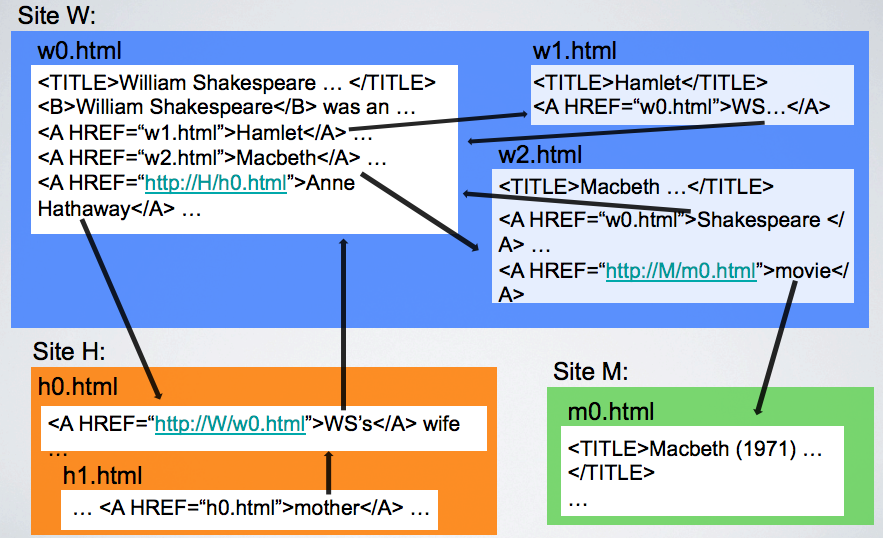
\includegraphics[width=0.5\textwidth]{images/l17-fig-1.png}
\end{figure}

Infine ci sono dei problemi legati all'autorevolezza e qualità delle pagine che non sempre è garantita, inoltre, la popolarità di una pagina non può essere usata come indice della sua qualità, perché potrebbe essere una pagina di spam.

\textbf{{\color{Red} Possibile esercizio:}} Quali sono le differenze più significative fra il reperimento delle informazioni su collezioni di documenti testuali locali e su Web?

\section{La struttura del Web}

Il web nasce con il contesto di iper-testo, ovvero con l'idea di poter consultare documenti che sono correlati tra di loro. Se un documento non ha dei collegamenti dall'esterno, questo non è accessibile.

\begin{figure}[htbp]
	\centering
	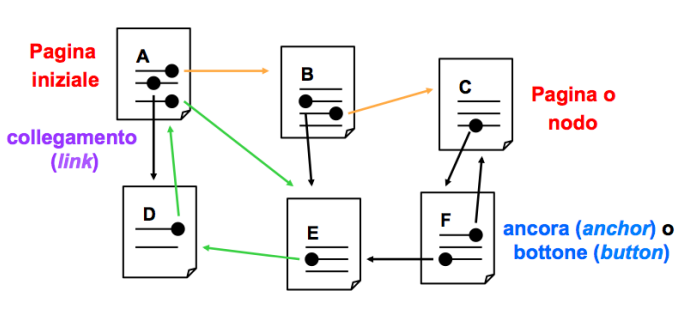
\includegraphics[width = 0.5\textwidth]{images/l17-fig-2}
\end{figure}

Un po' di terminologia:

\begin{itemize}
	\item \textbf{Pagina} o \textbf{nodo}: sinonimi che indicano un elemento o documento unitario dell'ipertesto che può essere utilizzato da un utente finale nella consultazione o navigazione. \`E una singola porzione atomica dell'ipertesto.
	\item \textbf{Ipertesto}: documento complesso organizzato con una struttura reticolare.
	\item \textbf{Collegamento} o \textbf{link}: le singole e diverse parti di un ipertesto sono organizzate in modo indipendente, poi vengono collegate fra di loro attraverso dei collegamenti o rimandi denominati link, che guidano il fruitore dal un nodo all'altro. Da notare che a livello implementativo i collegamenti non esistono, vengono infatti implementati utilizzando degli indirizzi per riferire i vari nodi.
	\item \textbf{Ancora} o \textbf{bottone}: il simbolo che indica al fruitore che da una specifica porzione di un nodo è stato attuato un collegamento con un altro nodo.
\end{itemize}

L'insieme delle pagine web e dei vari collegamenti può essere rappresentato come un grafo orientato (\textbf{web graph}) dove ogni nodo rappresenta una pagina e c'è un arco diretto tra un nodo ed un altro solo se c'è un collegamento che da una pagina va all'altra.
Ovviamente questo grafo è dinamico in quanto l'insieme delle pagine web è in continua evoluzione.

La modellazione come grafo è utile per formalizzare alcune misure della rilevanza, come il PageRank.

\begin{figure}[htbp]
	\centering
	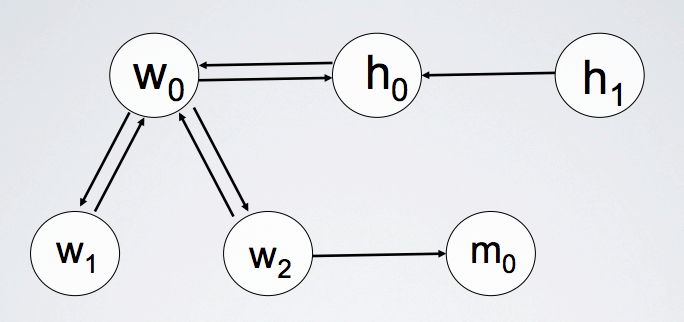
\includegraphics[width = 0.5\textwidth]{images/l17-fig-3}
\end{figure}

Le pagine presenti nel web possono essere:

\begin{itemize}
	\item \textbf{Statiche}: il contenuto della pagina è preparato e reso disponibile prima di una qualsiasi richiesta di un browser (o crawler).
	\item \textbf{Dinamico}: il contenuto della pagina è generato al momento della richiesta e dipende in parte dalla tipologia di richiesta effettuata e dal momento in cui questa viene fatta.
\end{itemize}

Per un crawler questa differenza non è importante per discriminare il contenuto della pagina, perché alla fine quello che interessa sono le informazioni presenti, non come la pagina viene generata.
Tuttavia bisogna tenere in considerazione che il contenuto di una pagina dinamica può cambiare nel tempo.

\subsection{Il web nascosto}

Molte pagine web fanno parte del \textbf{deep web}, ovvero una porzione di internet che non è normalmente raggiungibile perché le pagine al suo interno non sono \textit{puntante} da link presenti in altre pagine, oppure perché sono protette da password, oppure perché sono su server accessibili solamente all'interno di una rete privata. Un altro esempio di queste pagine sono quelle che vengono generate in risposta ad una determinata query.

Tutte queste pagine possono avere contenuti interessanti per un crawler, ma tipicamente è impossibile indicizzarle.

\subsection{La dimensione del web}

Data la sua dinamicità è difficile stimare la dimensione effettiva, inoltre, possono esserci pagine con contenuti di interesse limitato e altre molto più interessanti.

Se ci si limita a queste ultime, la dimensione del web può essere stimata considerando l'\textbf{Indexable Web} (\textbf{IW}) pubblico, ovvero quella parte di web che è indicizzata dai principali motori di ricerca, sia generalistici che specialistici.

La necessità di stimare la dimensione del web deriva dal fatto che è utile per stimare:

\begin{itemize}
	\item il tempo necessario alla raccolta delle pagine web d'interesse.
	\item la banda necessaria ad acquisire i vari documenti. Questi documenti possono trovarsi sparsi per il mondo, in zone con una connessione ad internet limitata.
	\item la quantità di memoria necessaria alla gestione e funzionamento del motore di ricerca.
\end{itemize}






















% !TEX encoding = UTF-8
% !TEX TS-program = pdflatex
% !TEX root = computabilità e algoritmi.tex
% !TEX spellcheck = it-IT
\chapter{Programmi generici - Lezione 18}

\section{Enumerazione dei programmi}

\textbf{Enumerazione delle funzioni calcolabili}: Un insieme \textit{X} è numerabile se esiste una funzione $ f : \mathbb{N} \rightarrow X $ suriettiva tale che $ \underbrace{f(0), f(1), f(2), \ldots}_{\mathbb{N}} $.


\subsection{Enumerazioni di supporto}
Per poter enumerare e quindi codificare dei programmi è necessario prima definire alcune funzioni biunivoche di supporto:

\begin{enumerate}
	\item $ \Pi : \mathbb{N}^2 \rightarrow \mathbb{N}$
	\item $ \nu : \mathbb{N}^3 \rightarrow \mathbb{N}$
	\item $ \tau : \bigcup\limits_{k \geq 1}\mathbb{N}^k \rightarrow \mathbb{N}$
\end{enumerate}

\subsubsection{$1. \Pi $}

Già osservata precedentemente, ovvero è la codifica delle coppie:

\begin{align*}
\Pi(x, y) &= 2^x(2y + 1) - 1\\
\Pi^{-1}(n) &= (\Pi_1(n), \Pi_2(n))
\end{align*}

\subsubsection{$2. \nu $}

$\nu $ può essere definita utilizzando $ \Pi $:

\begin{align*}
\nu(x_1, x_2, x_3) &= \Pi(\Pi(x_1,x_2), x_3) \\
\nu'(n) &= (v_1(n), v_2(n), v_3(n)) \\
\nu_1(n) &= \Pi_1(Pi_1(n))
\end{align*}

\subsubsection{$3. \tau $}

$ \tau $ può essere definita come $ (x_1, \ldots, x_k) \rightsquigarrow \prod\limits{i=1}^{k} = P_{i}^{x_i} -1$ ma questa funzione non è iniettiva:

\begin{align*}
(2,1) &= 2^2 \cdot 3^1 -1 \\
(2,1,0) &= 2^2 \cdot 3^1  \cdot 5^0 -1
\end{align*}

pertanto è necessario utilizzare

$$
\tau(x_1, \ldots, x_k) \rightsquigarrow \prod\limits{i=1}^{k-1} = P_{i}^{x_i} \cdot P_{k}^{x_k} - 2
$$

Per decodificare un numero \textit{n} è necessario prima calcolare la lunghezza della decodifica:

$$
l(n) = \max k.P.k \text{ divide } (n+2) \text{ con } k \leq n
$$

Anche se si tratta di una massimizzazione limitata è possibile dimostrare che è calcolabile sfruttando la minimalizzazione limitata, e quindi $ l(n) \in \mathcal{PR} $.

$$
a(n,i) = \begin{cases}
(n+2)_i &\text{ se } i < l(n)\\
(n+2)_i -1 &\text{ se } i = l(n)
\end{cases}
$$

l'inversa di $ \tau $ può essere definita come:

$$
\tau^{-1}(n) = \Big(a\big(n,1\big), a\big(n,2\big), \ldots, a\big(n,l(n)\big)\Big)
$$

\subsection{Enumerazione dei programmi}

Grazie alle funzioni precedentemente definite è possibile definire delle codifiche biunivoche che permettono di codificare con un numero sia una singola istruzione URM, sia un qualsiasi programma URM in $ \mathcal{P} $.

$$
\beta = \text{Ist URM} \rightarrow \mathbb{N} \quad \text{e} \quad \gamma \mathcal{P} \rightarrow \mathbb{N}
$$

\subsubsection{$ \beta = \text{Ist URM} \rightarrow \mathbb{N} $}

\begin{align*}
Z(n) &\rightarrow 4\cdot(n-1) \\
S(n) &\rightarrow 4\cdot(n-1)+1 \\ 
T(m,n) &\rightarrow 4\cdot\big(\Pi(m-1,n-1)\big)+2 \\
J(m,n,t) &\rightarrow 4\cdot\big(\tau(m-1,n-1,t-1)\big)+3
\end{align*}

I vari $ -1 $ servono perché i registri URM partono da 1, mentre la codifica deve partire da 0, altrimenti non sarebbe biunivoca.

La moltiplicazione per 4 serve per ``\textit{fare spazio}'' nella codifica in modo da continuare ad avere una funzione biunivoca. Allo stesso scopo servono anche le somme finali.

per fare l'inversa di $ \beta $ basta calcolare $ r = rm(4,n) $ e $ q = qt(4,n) $:

$$
\beta^{-1} \begin{cases}
Z(q+1) &\text{ se } r=0 \\
S(q+1) &\text{ se } r=1 \\
T\big(\Pi_1(q)+1, \Pi_2(q)+1\big) &\text{ se } r=2 \\
J\big(a(q,1)+1,a(q,2)+1,a(q,3)+1\big)&\text{ se } r=3
\end{cases}
$$
\todo{Verificare J}

In questo modo si ha una codifica per le istruzioni che permette di trasformare una sequenza di istruzioni in una sequenza di numeri

\subsubsection{$ \gamma \mathcal{P} \rightarrow \mathbb{N} $}

$$
\gamma(P) = \tau\big(\beta(I_1), \beta(I_2), \ldots\big)
$$

inversa con:

$$
\gamma^{-1}(n) = \tau^{-1}(n) = \Big(a\big(n,1\big), a\big(n,2\big), \ldots, a\big(n,l(n)\big)\Big)
$$

\section{Verso il programma 33 e la sua funzione}

Con quanto a disposizione si può parlare del programma 33, ottenuto decodificando il numero 33.

Prima di continuare serve della notazione aggiuntiva:

Dato $ P \in \mathcal{P} $, $ \gamma(P) $ indica il codice di \textit{P} e prende il nome di \textbf{G\"odel number}.

Dato \textit{n}, $ \gamma^{-1}(n) $ rappresenta il programma codificato nel numero \textit{n}, tale programma viene indicato con $ P_n $.

Un esempio è dato da:
\begin{lstlisting}[language=URM]
P:
T(1,2) 		--> 4Pi(1-1, 2-1) +2= 10
S(2)		  --> 4(2-1) = 4
T(2,1)   	--> 4Pi(2-1,1-1) +2= 6
\end{lstlisting}

\begin{align*}
\gamma(P) &= \tau(10,4,6)\\
&= 2^10 + 3^4 + 5^{6+1} -2\\
&= 19.439.999.998
\end{align*}

\begin{lstlisting}[language=URM]
P':
S(1)		--> 2
\end{lstlisting}

$$
\gamma(P’) = \tau(P) = 2
$$

I numeri $ 19.439.999.998 $ e $ 2 $ rappresentano due programmi che calcolano la stessa funzione successore.

Si può fare anche l'operazione inversa:

\begin{verbatim}
100
gamma^{-1}(100)  100+2
= 2^1 + 3^1 + 17 ^1
P1^1 P2^1 P3^0 P4^0 P5^0 P6^0 P7^1
1 -> S(1)
1 -> S(1)
0 -> Z(1)
0 -> Z(1)
0 -> Z(1)
0 -> Z(1)
1 -> S(1)
\end{verbatim}

Il numero $ 100 $ rappresenta quindi il programma che calcola la constante 1.

Dal momento che è possibile codificare i programmi in un numero, viene indotta anche un'enumerazione sulle funzioni calcolate da questi programmi:

Fissata $ \gamma : \mathcal{P} \rightarrow \mathbb{N} $, si ha:

$$
\phi_{n}^{(k)} = f_{P_n}^{(k)}
$$

ovvero $ \phi_{n}^{(k)} $ è la funzione di \textit{k} argomenti calcolata da $ P_n = \gamma^{-1}(n) $.
Per questa funzione è possibile definire anche 

$$
W_{n}^{(k)} = dom(\phi_{n}^{(k)}) \subseteq \mathbb{N}^k = \{\vec{x}\: | \: \vec{x} \in \mathbb{N}^k \text{ tale che } \phi_{n}^{(k)}(\vec{x}) \downarrow\}
$$

$$
E_{n}^{(k)} = cod(\phi_{n}^{(k)}) = \{y\:|\: \exists\vec{x} \: \phi_{n}^{(k)}(\vec{x}) = y  \}
$$

Ad esempio:

\begin{align*}
P: S(1) &\rightarrow \gamma(P) = 2 \\
\phi_{2}^{(1)}(x) &= x+1 \\
W_{2}^{(1)} &= \mathbb{N} \\
E_{2}^{(1)} &= \mathbb{N} - \{0\} \\
\end{align*}

Inoltre, si può definire una sorta di funzione di ordine superiore che, una volta fissato un $ k \geq 1$, associa un numero $ \mathbb{N} $ ad una funzione in $ \mathcal{C}^{(k)} : n \rightarrow  \phi_{n}^{(k)}$. Questa funzione è suriettiva perché data $ f \in \mathcal{C}^{(k)} $ esiste un programma \textit{P} che calcola $ f = f_{P}^{(k)} = \phi_{\gamma(P)}^{(k)} $ .
Questa funzioni non è iniettiva perché una stessa funzione può essere calcolata da più programmi.

Quindi 

$$
|\: \mathcal{C}^{(k)}\:| =  |\: \mathbb{N}\:| \leq |\: \mathcal{C}\:| = |\: \bigcup\limits_{k \geq 1} \mathcal{C}^{(k)} \:| = |\: \mathbb{N}\: |
$$
\todo{Verificare}

ovvero esistono delle funzioni che non sono calcolabili.














% !TEX encoding = UTF-8
% !TEX program = pdflatex
% !TEX root = InformationRetrieval.tex
% !TEX spellcheck = it-IT

\chapter{Anatomia e performance di un sistema di IR}

Nel nostro progetto noi non stiamo misurando lo stemmer di per se, ma stiamo misurando quanto lo stemmer migliora i risultati del sistema rispetto all'esecuzione senza stemming.

Si ha però che il sistema è composto da molti blocchi: tokenizzatore, stoplist, stemmer, modello e quindi non è semplice valutare il singolo componente, perché le prestazioni del sistema possono essere influenzate dagli altri componenti o dai parametri con i quali sono configurati.

Le misure nell'IR sono quindi misure end-to-end che considerano la totalità del sistema. Per valutare un singolo componente stabilisco quindi una pipeline di componenti e vario solamente quello che voglio misurare.

\section{Grid@CLEF}

L'idea è quindi quello di sviluppare un sistema di testing che funzioni con più lingue (MLIA: Multilingual Information Access) per capire come migliorare le performance dei singoli componenti.

Questo si può ottenere conducendo una serie di griglie di esperimenti, sistematici e ripetibili, su diversi linguaggi e con diversi componenti, effettuando uno sforzo comunitario per valutare sia i singoli componenti che la loro interazione con li altri.

Per implementare questo sistema è stata sviluppata una soluzione asincrona, basata su una produzione di dump intermedi XML, da scambiare tra i vari gruppi di ricerca. Ad esempio quelli che lavoro su un tokenizzatore, possono fornire i loro output ad un gruppi di ricerca che lavora agli stemmer per il tedesco.

Ci sono stati dei problemi implementativi però qualcosa si è riuscito a fare.

Mancava però una metodologia per analizzare i risultati di questi esperimenti.

\todo{aggiungere SIGIR RIGOR 2015}

\section{Valutazione delle performance - General Linear Mixed Model}

Posso combinare i dati dell'esecuzione dei vari sistemi della griglia in una matrice in cui le righe rappresentano i topic e le colonne sono i vari sistemi. Il valore delle cella è dato dall'average precision del sistema sul dato topic.
La matrice poi può essere plottata in una heat map, in modo che sia più comprensibile.

% immagine heatmap

Si può notare che la variazione è maggiore al variare dei topic, ovvero sistemi diversi tendono ad avere prestazioni simili sullo stesso topic.
Questo perché le performance del sistema dipendo sia dalla struttura del sistema, che dalla difficoltà del topic.

\todo{traduci slide 18 o 22 e copia le formule dalle slide successive}

















% !TEX encoding = UTF-8
% !TEX TS-program = pdflatex
% !TEX root = computabilità e algoritmi.tex
% !TEX spellcheck = it-IT

\chapter{Esercizi in preparazione al parziale}


\section{Teorema SMN}

\subsection{Esercizio 1}

Dimostrare che esiste $ S : \mathbb{N} \rightarrow \mathbb{N}$ tale che $|\: W_{S(x)}\:|  = 2 x$ e $ |\: E_{S(x)}\:| =x $

\subsubsection{Soluzione}

Si cerca una funzione $ f(x,y) $ che con $ x $ fissato abbia esattamente le caratteristiche richieste, ci pensa il teorema SMN a fare il resto.

\begin{align*}
f(x,y) &= \begin{cases}
y \dotminus x, &\text{ se } y < 2x \\
\uparrow, &\text{altrimenti}
\end{cases} \\
 &= y\dotminus x + \underbrace{\mu z. y +1 -2x}_{\text{fa divergere se } y \geq 2x}
\end{align*}

Questa funzione è calcolabile e quindi per il teorema SMN esiste $ S : \mathbb{N} \rightarrow \mathbb{N} $ tale che 

$$
\phi_{S(x)}(y) = f(x,y)
$$

e per costruzione $W_{S(x)} = [0,2x-1]$ e $ E_{S(x)} = [0,x-1] $.

\section{Calcolabilità delle funzioni}

\subsection{Esercizio 1}

Dimostrare che 

$$
f(x) = \begin{cases}
\phi_x(x) &\text{se} \phi_x(x)\downarrow \\
0 &\text{altrimenti}
\end{cases}
$$

non è calcolabile.

\subsubsection{Soluzione}

Non si può usare il \textit{trick} della diagonale, perché la funzione deve essere proprio uguale alla diagonale.

$$ h(x) = f(x)+1 = \begin{cases}
\phi_x(x)  + 1 &\text{se} \phi_x(x)\downarrow \\
1 &\text{altrimenti}
\end{cases}
 $$

Così facendo $ h \neq \phi_x(x) \forall x $ e pertanto non è calcolabile.

Ma $ h $ è il successore di $ f $, quindi $ f $ non può essere calcolabile, perché se così non fosse $ h(x) = f(x) +1 $ sarebbe calcolabile per composizione di funzioni calcolabili.ò

Da notare che questa cosa non vale in se e solo se:

$$ h(x) = f(x) +1 \text{ non calcolabile }\Rightarrow f(x)  \text{ non calcolabile } $$

ma \textbf{NON \`{E} VERO}

$$ f(x) \text{ non calcolabile } \Rightarrow f(x) = h(x) +1 \text{ non calcolabile }$$
%------------

\subsection{Esercizio 2}

Sia $ \mathbb{P} $ l'insieme dei numeri pari, dimostrare che la funzione caratteristica è primitiva ricorsiva.

$$
\mathcal{X}_\mathbb{P} = \begin{cases}
1 &\text{ se $ x $ è pari} \\
0 &\text{ altrimenti}
\end{cases}
$$

\subsubsection{Soluzione}

\begin{align*}
\mathcal{X}_\mathbb{P}(0) &= 1
\mathcal{X}_\mathbb{P}(x+1) &= \overline{sg}\big(\mathcal{X}_\mathbb{P}(x)\big)
\end{align*}

Dal momento che in un esercizio non sappiamo dell'esistenza del segno negato è necessario andare a mostrare che anche quella funzione è primitiva ricorsiva:

\begin{align*}
 \overline{sg}(0) &= 1 \\
  \overline{sg}(x+1) &= 0
\end{align*}


\subsection{Esercizio 3}

Dimostrare che la funzione $ half(x) = \lfloor\frac{x}{2}\rfloor $ è primitiva ricorsiva.

\subsubsection{Soluzione}

\begin{align*}
half(0) &= 0 \\
half(x+1) &= half(x) + rm_2(x)
\end{align*}

come prima bisogna dimostrare che $ rm_2 $ è ricorsiva primitiva

\begin{align*}
rm_2(x) &= 0
rm_2(x+1) &= \overline{sg}(rm_2(x))
\end{align*}

ma anche $ \overleftarrow{sg} $ è in $ \mathcal{PR} $

\begin{align*}
\overline{sg}(0) &= 1 \\
\overline{sg}(x+1) &= 0
\end{align*}

\section{Macchina URM}

\subsection{Esercizio 1}

Consideriamo la macchina $ \text{URM}^- $ che al posto dell'istruzione successore ha quella che effettua il predecessore.
Come sono in relazione le due classi? 

Ovvero:
 $$\mathcal{C}^- \text{ ? } \mathcal{C}$$
 
 \subsubsection{Soluzione}
 
 \`{E} chiaro che  $\mathcal{C}^- \subseteq \mathcal{C}$ perché la funzione predecessore può essere sostituita da un programma che calcola il predecessore.
 
 Per vedere \textbf{se}  $\mathcal{C}^- \supseteq \mathcal{C}$ bisogna provare a simulare il successore con un programma per la macchina $ \text{URM}^- $.

Ma dato un $ P \in \text{URM}^- $ qualsiasi $ P(\vec{x}) $ dopo $ n $ passi, $ \forall n $, tutti i registri $ r_i \leq \max x_i$.

Se $ n = 0 $ è ovvio perché i registri non cambiano.

Se $ n \rightarrow n+1 $, l'istruzione aggiunta può essere:
\begin{itemize}
	\item precessore ma il valore non aumenta
	\item zero azzera un registro
	\item il trasferimento non incrementa i valori
\end{itemize}

Dal momento che i registri di un programma in $ \text{URM}^- $ non aumentano mai, non è possibile implementare la funzione successore, quindi \textbf{non vale} la relazione $\mathcal{C}^- \supseteq \mathcal{C}$.


\subsection{Esercizio 2}
$ \text{URM}^S$ che non ha \texttt{S(n)} e \texttt{J(m,n,t)} ma ha \texttt{JS(m,n,t)} che prima fa il test e poi incrementa il registro $ m $.

\subsubsection{Soluzione}

$\mathcal{C}^S \subseteq \mathcal{C}$ perché un programma URM riesce ad emulare l'istruzione \texttt{JS}.

$\mathcal{C}^S \supseteq \mathcal{C}$ non vale, perché un programma $ \text{URM}^S$ non riesce a calcolare la funzione successore.


\section{Diagonalizzazione}

\subsection{Esercizio 1}

$ F_0 = \{f \: | \: \text{cod}(f) \subseteq \{0\} \text{ e parziali}\}$ è numerabile?

\subsubsection{Soluzione}

L'unica differenza tra queste funzioni è data dai domini che sono tanti quanti i numeri naturali.

Suppongo per assurdo che $ F_0 $ sia enumerabile, allora:

\begin{verbatim}
		f0	f1 f2
0      0   0   0
1      0   0
2
\end{verbatim}

considerando la diagonale, posso definire

$$
f(x) = \begin{cases}
0 &\text{se } f_x(x)\uparrow \\
\uparrow &\text{se } f_x(x)=0
\end{cases}
$$

$ f $ dovrebbe appartenere a $ F_0 $ ma per costruzione non compare nella enumerazione, quindi $ F_0 $ non è enumerabile.

\subsection{Esercizio 2}

$ f : \mathbb{N} \rightarrow \mathbb{N} $ totale e decrescente se $ \forall x,y \: x \leq y \Rightarrow f(y) \leq f(x) $.

$ F_d = \{ f : \mathbb{N} \rightarrow \mathbb{N} \: \ \: f \text{ totale e descrescente e } \text{cod}(f) \subseteq \{0,1\} \} $ è numerabile?

\subsubsection{Soluzione}

Le funzioni dell'insieme possono essere o costanti uguali a 0 o 1, oppure uguali a 1 fino ad un certo valore per poi diventare costanti a 0.

$$ \forall f \in F_d \: n(f)  = \text{sup}(\{x \: | \: f(x) = 1\})$$

$ n(f) $ è il punto in cui cambia il valore della funzione e caratterizza $ f $, ovvero

$$
\forall f_1, f_2 \in F_d \: n(f_1) = n(f_2) \Rightarrow f_1 = f_2
$$

quindi $ n : F_d \rightarrow \mathbb{N} \cup \{\infty\} $ è una funzione iniettiva e suriettiva, pertanto $ |\: F_d \:| = |\: \mathbb{N} \cup \{ \infty \} \:| $, ovvero $ F_d $ è numerabile.


\subsection{Esercizio 3}

Trovare $ f : \mathbb{N} \rightarrow \mathbb{N} $ totale e non calcolabile tale che $ f(x)  =x $ per infiniti $ x $.

\subsubsection{Soluzione}

$$
f(x) = \begin{cases}
x, &\text{ se $ x $ è pari} \\
\phi_{\frac{x-1}{2}}(x) +1, &\text{ se } \phi_{\frac{x-1}{2}}(x) \downarrow \\
0, &\text{ se } \phi_{\frac{x-1}{2}}(x) \uparrow 
\end{cases}
$$

\subsection{Esercizio 4}

Trovare una funzione $ f $ crescente, totale e non calcolabile.

\subsubsection{Soluzione}

$$
h(x) = \begin{cases}
\phi_x(x)+1, &\text{ se }\phi_x(x)\downarrow \\
0, &\text{ se } \phi_x(x) \uparrow
\end{cases}
$$

$ h $ è non calcolabile perché è definita sulla diagonale distorta.

$$
f(x) = \sum\limits_{y \leq x} h(y)
$$

Così definita $ f $ è:
\begin{itemize}
	\item totale
	\item crescente: $ f(x+1) = f(x) + h(x+1) \geq f(x) $
	\item $ \forall x $ se $ \phi_x(x) \downarrow \: f(x) = \sum\limits_{y \leq x} h(y) \geq h(x) = \phi_x(x) +1 \neq \phi_x(x) $ e se $ \phi_x(x) \uparrow $, $ h(x) = 0 \neq \phi_x(x) $, ovvero $ f $ non è calcolabile.
\end{itemize}

\subsection{Esercizio 5}

Può esistere $ f : \mathbb{N} \rightarrow \mathbb{N} $ non calcolabile tale che $ \forall g : \mathbb{N} \rightarrow \mathbb{N} $ non calcolabile $ f+g  $ è calcolabile?

$$
(f+g)(x) = f(x) + g(x)
$$

\subsubsection{Soluzione}

Non può esistere, perché per assurdo, sia $ f $ una funzione tale che $ (f+f) $ è calcolabile:

\begin{align*}
h(x) &= f(x) + f(x) \\
		&= 2 f(x)
\end{align*}

$h(x)$ è quindi calcolabile, però utilizzando questa funzione si può definire $ f(x) = qt(2, h(x)) $, dimostrando la calcolabilità di $ f $ che per ipotesi non è calcolabile.



%% !TEX encoding = UTF-8
% !TEX TS-program = pdflatex
% !TEX root = computabilità e algoritmi.tex
% !TEX spellcheck = it-IT

\section{Correzione compitino}

\subsection{Esercizio 1}

Definire la classe delle funzioni ricorsive e dimostrare che $ pow2(y)  \in \mathcal{PR} $

\subsubsection{Soluzione}

La definizione è negli appunti.

Per dimostrare che la funzione è primitiva ricorsiva la si definisce per ricorsione primitiva:

$$
\begin{cases}
pow2(0) &= 1 \\
pow2(y+1) &= double(pow2(y))
\end{cases}
$$

Serve definire anche $ double $ come primitiva ricorsiva:

$$
\begin{cases}
double(0) &= 0 \\
double(y+1) &= S(S(double(y)))
\end{cases}
$$

$ pow2 $ è quindi primitiva ricorsiva.

\subsection{Esercizio 2}

Analizzare la classe delle funzioni calcolabili $ \mathcal{C}' $ associate alla macchina URM' che al posto dell'istruzione di salto e dell'istruzione successore ha l'istruzione \texttt{JI(m,n,t)} che se trova i due registri uguali, prima incrementa il registro \texttt{m} e poi effettua il salto all'istruzione \texttt{t}.

\subsubsection{Soluzione}

Le istruzioni \texttt{J} e \texttt{S} della macchina URM possono essere replicate con 

\begin{lstlisting}[language=URM]
// J(m,n,t)
T(m,k)
JI(k,n,t)
// S(n)
Il: JI(n,n,l+1)
\end{lstlisting}

Serve poi la prova induttiva sul numero di istruzioni che è sempre quella, l'importante è specificare che nei passi intermedi della dimostrazione si ottiene un programma ibrido.

C'è poi da fare la dimostrazione dell'altro verso, che avviene in modo analogo.

\subsection{Esercizio 3}

Può esistere una funzione $ f $ totale e non calcolabile tale che $ cod(f) = \mathbb{P} $.

\subsubsection{Soluzione}

Perché sia totale basta che sia sempre definita, per ottenere la non calcolabilità la devo rendere diversa da tutte le funzioni calcolabili.

$$
f(x) = \begin{cases}
x, &\text{se $ x $ è pari}\\
2(\phi_{\frac{x-1}{2}}(x) +1), &\text{se $ x $ è disparie e $ \downarrow $} \\
0, &\text{ altrimenti}
\end{cases}
$$

Ma anche una definizione più semplice va bene:

$$
f(x) = \begin{cases}
2 (\phi_x(x) +1), &\text{ se }\phi_x { è totale} \\
0, \text{ altrimenti}
\end{cases}
$$

\chapter{Funzione universale}

Vogliamo un programma universale che prende in input il numero del programma e l'input da utilizzare e fornisce in output il risultato dell'esecuzione del programma sul dato input.

$$
\Psi_U(x,y) = \phi_{x}(y)
$$

La funzione universale ha in generale $ k+1 $ argomenti:

\begin{align*}
\Psi_U^{(k)} &: \mathbb{N}^{k+1} \rightarrow \mathbb{N} \\
\Psi_U(e, \vec{x}) = \phi_{e}^{k}(\vec{x})
\end{align*}

\section{Calcolabilità della funzione universale}

Per calcolare $ \Psi_U(e, \vec{x}) = \phi_{e}^{k}(\vec{x}) $ è necessario come prima cosa recuperare il programma rappresentato da $ e $ utilizzando $ \gamma^{-1}(e) = P_e$.

Dopodiché è necessario eseguire $ P_e(\vec{x}) $, la quale può produrre un output $\phi_{e}^{k}(\vec{x}) = \Psi_U(e, \vec{x}) $ oppure può non terminare e in questo caso $ \Psi_U(e, \vec{x})\uparrow $.

\subsection{Dimostrazione pseudo-formale}

\begin{verbatim}
	|r1|r2|r3|...|0|...
\end{verbatim}

$ C = \prod_{i \geq 1} = p_{i}^{r_i} $ con questa codifica della memoria è possibile accedere al contenuto del registro $ i $-esimo con $ r_i = (C)_i$.

Qualcosa sulla codifica dello stato del programma: s$ \sigma = \Pi(C,J) $.

$ C_k(e,\vec{x}, t)  = $ contenuto dei registri dopo $ t $ passi del programma $ P_e $ sull'input $ \vec{x} $.

$ J_k() = \begin{cases}
&\text{istruzione da eseguire dopo di passi di } P_e(\vec{x}) \text{, se non termina.}\\
&0 \text{ altrimenti}
\end{cases} $ 

C'è da dimostrare che $ C_k, J_k \in \mathcal{PR} \subseteq \mathcal{R}  = \mathcal{C}$, una volta fatto ciò è possibile definire:

$$
\Psi_U(e, \vec{x}) = \phi_{e}^{k}(\vec{x}) = \Big( C_k(e,\vec{x}, \mu t.J_k(e,\vec{x},t)) \Big)_1 \in \mathcal{R} = \mathcal{C}
$$

Sulla base di $ C_p(\vec{x},t) $ e $ J_p(\vec{x}, t) $ si possono definire per ricorsione primitiva:

$$
C_p()
$$


Servono prima un po' di funzioni ausiliarie.

Argomenti di un istruzione URM $i = \beta(\text{Istr}) $
\begin{align*}
	Z_{arg}(i) &= qt(4,i) +1 \\
	S_{arg}(i) &= qt(4,i) +1 \qquad \qquad i = (n-1)\times 4 \\
	T_{arg_1} &= \Pi_1 (qt(4,i)) +1 \qquad \qquad i =\ldots \\
	T_{arg_2} &= \Pi_2 (qt(4,i)) +1
\end{align*}

Effetto dell'esecuzione di un istruzione:

$$
zero(C,n) = qt(p_{n}^{(C)_n} , C)
$$

$$
succ(C,n) = p_n \cdot C
$$

$$
trasf(C,m,n) = zero(C,n) \cdot p_{n}^{(C)_m}
$$

Effetto dell'esecuzione di un istruzione $ i = \beta(\text{Itrs})$:

$$
change : \mathbb{N}^2 \rightarrow \mathbb{N}
$$

$$ 
change(C,i) = \begin{cases}
zero(C, Z_{arg}(i)) se \: rm(4,i) = 0 \\
succ(C, S_{arg}(i)) se \: rm(4,i) = 1 \\
trasf(C, T_{arg_1}(i), T_{arg_2}(i)) se rm(4,i) = 2 \\
C altrimenti (il salto non cambia la configurazione di memoria)
\end{cases}
$$ 


Prossima configurazione di memoria

\begin{align*}
nextconf(e, C, t) &= \text{Configurazione dei registri al prossimo passo partendo da } C \text{ e eseguendo la \textit{t}-esima istruzione di }P_e \\
	&= change(C, a(e,t))
\end{align*}

dove \textit{a} è la funzione che data la codifica di un programma ritorna il codice della $ t $-esima istruzione.

$ is(C,i,t) =$ numero dell'istruzione successiva se al passo corrente eseguo $ i = \beta(\text{Istr}) $ che si trova in posizione $ t $ del programma.

$$
is(C,i,t) = \begin{cases}
t+1, &\text{se } rm(4.i) \neq 3 \text{ oppure } (C)_{J_{arg_1}(i)} \neq (C)_{J_{arg_2}(i)}  \\
J_{arg_3}(i), &\text{ altrimenti}
\end{cases}
$$ 

$$
nextistr(e, C, t) = \text{prossima istruzione a partire da C ed eseguendo t}
$$

$$
nextistr(e,C,t) =\begin{cases}
is(C, a(e,t), t ), &\text{ se } is(C, a(e,t), t ) \neq l(e) +1 \\
0, &\text{ altrimenti}
\end{cases} 
$$

Siamo quasi alla fine

\begin{align*}
C_k (e, \vec{x}, 0) &= \prod\limits_{i=1}^{k} p_{i}^{r_i}\\
J_k(e,\vec{x}, 0) &= 1 \\
C_k (e, \vec{x}, t+1) &= nextconf(e, C_k(e,\vec{x}, t) , J_k(e, \vec{x}, t)) \\
J_k(e,\vec{x}, t+1) &= nextistr(e, C_k(e, \vec{x}, t) , J_k(e, \vec{x}, t)) 
\end{align*}

Dato che tutte le funzioni utilizzate, anche $ C_k $ e $ J_k $ sono primitive ricorsive e quindi calcolabili.

$$
\Psi_{U}^{(k)} = \Big(  C_k(e, \vec{x}, \mu t.J_k(e, \vec{x}, t)) \Big)_1 \in \mathcal{R}
$$



\section{Corollari-rio}

Sono decidibili i seguenti predicati

\begin{enumerate}
	\item $ H_k (e,\vec{x}, t) = P_e(\vec{x}) \downarrow $ in $ t $ o meno passi.
	\item $ S_k (e,\vec{x},y, t) = P_e(\vec{x}) \downarrow y $ in $ t $ o meno passi.
\end{enumerate}

Entrambi sono calcolabili perché basta fare andare il programma per $ t $ passi e osservare l'output.

$$
\mathcal{X}_{H_k}(e, \vec{x}, t) = \overline{sg}(J_k{e,\vec{x},t})
$$


$$
\mathcal{X}_{S_k}(e, \vec{x}, y, t) =  \overline{sg}((J_k(e,\vec{x},t)) + |\: y - (C_k(e,\vec{x},t) )_1\:|)
$$
%% !TEX encoding = UTF-8
% !TEX TS-program = pdflatex
% !TEX root = computabilità e algoritmi.tex
% !TEX spellcheck = it-IT

\section{Funzione inversa con i corollari}

Data una funzione $ f : \mathbb{N} \rightarrow \mathbb{N} $iniettiva, totale e calcolabile. Allora

$$ 
f^{-1}(y) =\begin{cases}
x \text{ tale che } f(x) = y \\
\uparrow \text{ altrimenti}
\end{cases}
$$

è calcolabile con

$$
f^{-1}(y) = \mu x. |\: f(x) - y\:|
$$

Però se \textit{f} non è totale, non è più garantita la calcolabilità.

L'idea è quindi quella di eseguire un certo numero di passi via via crescente su ogni programma. (In teoria questa cosa è già stata fatta. Però non si poteva spiegare in modo formale).

Essendo \textit{f} calcolabile questa sarà calcolata da un certo programma \textit{e}.

$$
f^{-1}(y) = \mu (x,t). S(e, x,y, t)
$$

Peccato che non esiste un operatore che minimizza le coppie. Neanche la minimalizzazione innestata funziona, perché scorrerei la tabella prima solo sulle colonne e poi solo sulle righe.

Serve quindi un barbatrucco, in modo da riuscire a codificare una coppia con un numero intero.

$$
\mu w.  S(e, (w)_1, y, (w)_2 )
$$

Ovvero del numero \textit{w} ci interessano solo gli esponenti dei primi due divisori primi del numero.
Piccola nota: usiamo un predicato nella minimalizzazione quando sarebbe necessario utilizzare una funzione. Sarebbe quindi più corretto utilizzare il valore assoluto della funzione caratteristica del predicato, meno uno.

$$
f^{-1}(y) = \Big( \mu w.  S(e, (w)_1, y, (w)_2 ) \Big)
$$

\section{Cose non calcolabili}

Ci sono un sacco di cose che non sono calcolabili e un sacco di cose non decidibili.\\

\subsection{Totalità di un programma}

Predicato $ Tot(x) = \phi_x \text{ è totale} $ non è decidibile.

\subsubsection{Dimostrazione}

Supponiamo per assurdo che $ Tot(x) $ sia decidibile.

Definiamo

$$
f = \begin{cases}
\phi_x(x) +1 \text{ se \textit{x} è totale}\\
1 \text{ altrimenti}
\end{cases}
$$

Questa funzione è certamente totale e $ f \neq \phi_x \forall x \text{ tale che } \phi_x \text{ è totale perché se }\phi_x $ è totale $ f(x) = \phi_x(x)+1 \neq \phi_x(x) $ e quindi non è calcolabile.

Sfruttando però la totalità di \textit{Tot} è possibile scrivere la funzione $ \phi_(x) \text{ come } \Phi_U(x,x)$ e quindi \textit{f} risulterebbe definita per casi, utilizzando solamente funzioni calcolabili e quindi anch'essa sarebbe calcolabile.
Non è però possibile utilizzare la classica aritmetizzazione dell'\textit{if}, perché quando $ \phi_x $ non è totale si ha un risultato indefinito.

$$
f(x)= \bigg( \mu w. \Big( S(x,x,(w)_1, (w)_2) \wedge Tot(x) \vee (w)_1 = 0 \wedge \neg Tot(x) \Big) \bigg)_1 +1
$$

Con questa definizione il programma $ \phi_x $ vengono eseguiti sempre un po' di passi alla volta, così quando $ Tot(x) $ non è totale viene ritornato il valore corretto.

\textit{f} risulta quindi calcolabile e questo è assurdo per costruzione di \textit{f}.

\subsection{Esercizio}


\textit{Q(x)} decidibile, f1,f2 N -> N calcolabili.  f(x) = f1(x) se Q(x), f2(x) altrimenti è calcolabile?

\todo[inline]{TODO}

\subsection{Esercizio - Terminazione del programma sul suo indice}

$H(x) = \phi_x(x) \downarrow$ non è decidibile.


\section{Operazioni effettive su programmi}

Dati due programmi $ P_x, P_y $ questi calcoleranno le due funzioni $\phi_x, \phi_y$.

$$
(\phi_x + \phi_y)(z) = \phi_x(z) + \phi_y(z) = \phi_e(z) = \phi_{k(x,y)}(z)
$$

Con \textit{K} funzione totale e calcolabile.

Ovvero esiste $ K : \mathbb{N}^2 \rightarrow \mathbb{N} $ tale che $ \phi_{k(x,y)}(z) = \phi_x(z) + \phi_y(z)$.

Questo si dimostra prima utilizzando il teorema SMN:

$$
g(x,y,z) = \phi_x(z) + \phi_y(z) = \Phi_U(x,z) + \Phi_U(y,z)
$$

è calcolabile e quindi per il teorema SMN esiste $ K : \mathbb{N}^2 \rightarrow \mathbb{N} $ totale e calcolabile tale che 

$$
g(x,y,z) = \phi_{K(x,y)}(z)
$$

\subsection{Funzione inversa}

Un ragionamento simile può essere fatto con la funzione inversa.

Esiste $ K : \mathbb{N} \rightarrow \mathbb{N} $ totale e calcolabile, tale che

$$
\phi_{K(x)}(y) = (\phi_x)^{-1}(y)
$$

Definisco quindi 

$$
g(x,y) =  (\phi_x)^{-1}(y) = \Big(\mu w. S\big(x,(w)_1, y, (w)_2\big)\Big)_1
$$

\textit{g} è calcolabile e quindi per il teorema SMN si ha che esiste $ K : \mathbb{N} \rightarrow \mathbb{N} $  calcolabile e totale, tale che

$$
g(x,y,z) = \phi_{K(x,y)}(z)
$$



\subsection{Programmi con lo stesso domino}

Esiste $ K : \mathbb{N}^2 \rightarrow \mathbb{N} $ totale e calcolabile, tale che

$$
W_{K(x,y)} = W_x \cup W_y
$$

ovvero si vuole che il programma composto abbia come dominio l'unione dei due domini.

Serve quindi una funzione per l'esecuzione dei due programmi passo passo:

$$
g(x,y,z) = \mathbb{1}(\mu w. ( H(x,z,w) \vee H(y,z,w)))
$$

questa funzione è definita se \textit{z} appartiene ad almeno uno dei due domini ed è indefinita se non compare in nessuno dei due domini.

$$
g(x,y,z) = \begin{cases}
1 \text{ se } z \in W_x \cup W_y \\
\uparrow \text{ altrimenti}
\end{cases}
$$

Essendo questa funzione calcolabile, per il teorema SMN esiste una funzione $ K : \mathbb{N}^2 \rightarrow \mathbb{N} $ totale e calcolabile tale che

$$
\phi_{K(x,y)}(z) = g(x,y,z)
$$

Così facendo si ottiene proprio la funzione desiderata perché

$$
z \in W_{K(x,y)} \Leftrightarrow \phi_{K(x,y)}(z)\downarrow \Leftrightarrow z \in W_x \cup W_y
$$

\subsection{Programmi con gli stessi codomini}

Esiste $ S : \mathbb{N}^2 \rightarrow \mathbb{N} $ totale e calcolabile tale che 

$$
E_{S(x,y)} = E_x \cup E_y
$$

L'idea è quella di eseguire $ P_x $ se $ z $ è pari altrimenti se è dispari viene eseguito $ P_y $. I due programmi devono però essere eseguiti su $ z/2 $ in modo che possano essere eseguiti su tutti i numeri.

$$
g(x,y,z) =\bigg( \mu w. \Big( \big(Pari(z) \wedge S(x,z/2, (w)_1, (w)_2)\big) \vee \big( \neg Pari(z) \wedge S(y,z/2, (w)_1, (w)_2) \big) \Big) \bigg)_1
$$

Si ha quindi che la funzione 

$$
g(x,y,z) = \begin{cases}
\phi_x(z/2) \text{se \textit{z} è pari} \\
\phi_y(z/2) \text{se \textit{z} è dispari}
\end{cases}
$$

è calcolabile per come è stata precedentemente definita. (Sarebbe da ricopiare la definizione, utilizzando \textit{qt} al posto della divisione classica).

Essendo calcolabile segue che per il teorema SMN esiste $ S : \mathbb{N}^2 \rightarrow \mathbb{N} $ calcolabile e totale, tale che

$$
\phi_{S(x,y)}(z) = g(x,y,z)
$$

ed è la funzione cercata perché:

$$
v \in E_{S(x,y)} \Rightarrow \exists z | \phi_{S(x,y)}(z) = v \Rightarrow \begin{cases}
g(x,y,z) = v = \phi_x(z/2) \text{ se \textit{z} è pari} \Rightarrow v \in E_x \\
g(x,y,z) = v = \phi_y(z/2) \text{ se \textit{z} è dispari} \Rightarrow v \in E_y 
\end{cases} \Rightarrow v \in E_x \cup E_y
$$

e vale anche l'altra inclusione, perché, sia $ v \in E_x $, esiste $ z $ tale che $ \phi_x(z) = v  \Rightarrow \phi_{S(x,y)}(2z) = g(x,y,2z) = \phi_x(z)$ e siccome per un qualche argomento \textit{z} si ha che $ v \in E_{S(x,y)} $.


\section{Esercizi}

\begin{enumerate}
	\item Esiste $ K : \mathbb{N} \rightarrow \mathbb{N} $ calcolabile e totale, tale che $ E_{K(x)} = W_x $?
	\item Data $ f : \mathbb{N} \rightarrow \mathbb{N} $ calcolabile, esiste $ K : \mathbb{N} \rightarrow \mathbb{N} $ calcolabile e totale, tale che $ \forall x \: W_{K(x)} = f^{-1}(W_x) $
\end{enumerate}









\part{Algoritmi}
% !TEX encoding = UTF-8
% !TEX TS-program = pdflatex
% !TEX root = computabilità e algoritmi.tex
% !TEX spellcheck = it-IT
\chapter{Lezione 2}
\section{Introduzione e Algoritmi sui grafi}\label{lezione-2---introduzione-e-algoritmi-sui-grafi}

C'è la possibilità di fare un pre-orale nella settimana dei compitini.

Libro: Cormen, Introduzione agli algoritmi e strutture dati
\href{http://catalogo.unipd.it/F/FCKK1DACESL2TDH5CF15FLDL2BUM936U1XG9U15MFDCKI764BV-10675?func=full-set-set\&set_number=011139\&set_entry=000001\&format=999}{BIB}:

\begin{itemize}
\item
  Introduzione agli algoritmi sui grafi
  \begin{itemize}
  \item
    Strutture dati per i grafi
  \item
    Operazioni elementari sui grafi
  \end{itemize}
\item
  Algoritmi su stringhe (capitolo 22)
\item
  Algoritmi paralleli (capitolo 27)
\item
  Algoritmi di geometria computazionale
\end{itemize}

\subsection{Terminologia dei grafi}\label{terminologia-dei-grafi}

Un grafo \emph{G} è costituito da un insieme di vertici \emph{V} e di
archi \emph{E}. Ad ogni arco vengono associati due vertici in \emph{V}.

Se c'è un ordine tra i due estremi degli archi, il grafo prende il nome
di \textbf{orientato} o \textbf{diretto}. In questo caso, il primo
vertice prende il nome di \textbf{coda} e l'ultimo \textbf{testa}.

Un \textbf{cappio} è un arco i cui due estremi coincidono.

Un grafo non orientato si dice \textbf{semplice} se non ha cappi e non
ci sono due archi con gli stessi estremi. Mentre se il grafo è
orientato, perché sia semplice non devono esserci archi con gli stessi
estremi, iniziali e finali. Un grafo non semplice prende il nome di
\textbf{multi-grafo}.

\begin{figure}[htbp]
\centering
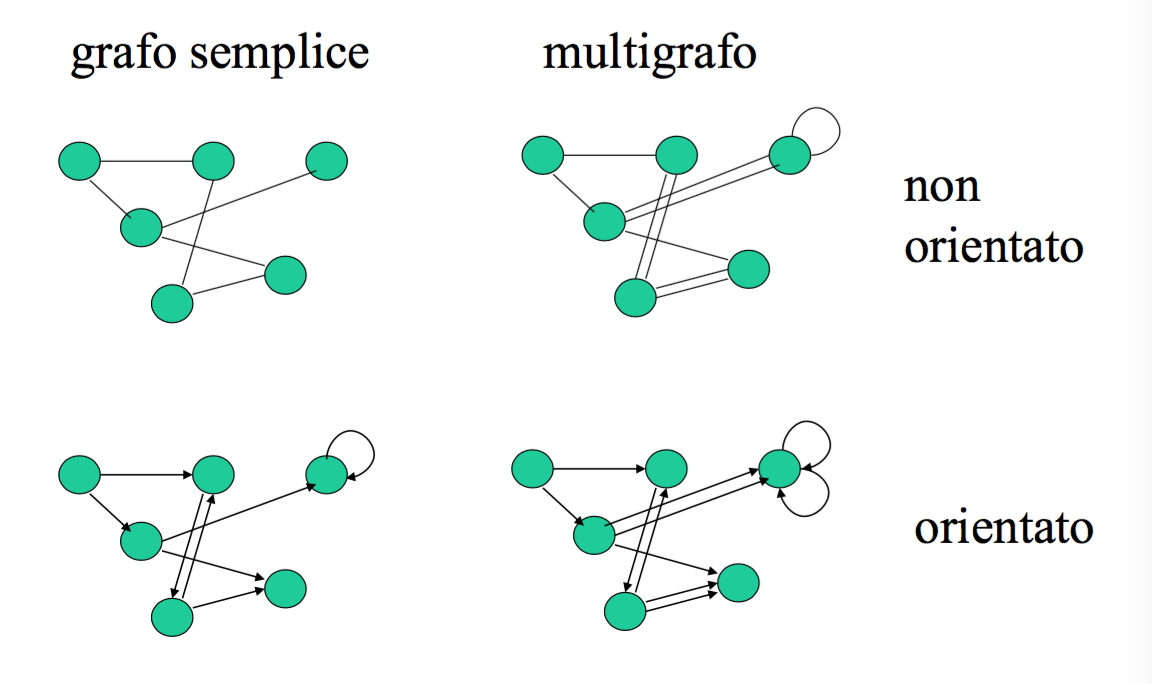
\includegraphics[width=0.75\textwidth]{./notes/immagini/l2-grafi.png}
\caption{Varie tipologie di grafi}
\end{figure}

Se un grafo è semplice, un arco può essere espresso con:

$$
e = uv \in E \text{, con } u,v \in V
$$

e si dice che l'arco \emph{e} è incidente in \emph{u} e \emph{v}. Da
notare che se il grafo è orientato
$e = uv \neq vu$ e la terminologia diventa
``l'arco \emph{e} esce da \emph{u} e entra in \emph{v}''.

Il \textbf{grado} di un vertice \emph{v} viene indicato con $\delta(v)$ e rappresenta il numero di archi incidenti in quel
vertice. Se il grafo è ordinato, il suo \textbf{grado uscente} $\delta^+(v)$ è il numero di archi uscenti e il suo \textbf{grado entrante} è $\delta^-(v)$.

Se due vertici sono collegati da un arco, questi vengono detti
\textbf{adiacenti}.

Un \textbf{cammino} di lunghezza \emph{k} da un vertice \emph{u} ad un
vertice \emph{v} in un grafo \emph{G=(V,E)}, è una sequenza di
\emph{k+1} vertici $x_0 \ldots x_k$, tali che 

$$x_0 = u$, $x_k = v$ e $x_{i-1}x_i \in E \forall i = 1\ldots k$$.

Se il cammino ha lunghezza 0, questo viene detto \textbf{nullo}, mentre
se il vertice di partenza coincide con quello di arrivo, il cammino
prende il nome di \textbf{chiuso}.

Un cammino viene detto \textbf{semplice} quanto tutti i vertici che lo
compongono sono distinti, ad eccezione del primo, che può coincidere
con l'ultimo. Un cammino semplice e il primo vertice coincide con
l'ultimo, questo prende il nome di \textbf{ciclo}. L'esempio più
semplice di ciclo è dato da un cappio.

Un grafo \textbf{aciclico} è un grafo che non contiene cicli.

Quando esiste almeno un cammino dal vertice \emph{u} al vertice
\emph{v}, si dice che \emph{v} è \textbf{accessibile} (o
\textbf{raggiungibile}) da \emph{u}. Questa definizione è simmetrica
solamente nel caso di un grafo non orientato.

Un grafo non orientato si dice \textbf{connesso} se esiste almeno un
cammino tra ogni coppia di vertici.

Le \textbf{componenti connesse} di un grafo sono le classi di
equivalenza dei suoi vertici rispetto alla relazione di accessibilità,
ovvero un sottoinsieme di vertici che sono tutti tra loro accessibili.

Nel caso di un grafo orientato, si dice che è \textbf{fortemente
connesso} se esiste almeno un cammino tra ogni vertice del grafo. In
modo analogo è possibile definire le \textbf{componenti fortemente
connesse}

Sia la \textbf{connessione} che la \textbf{connessione forte} hanno le
proprietà:

\begin{itemize}
\item
  \textbf{riflessiva}: se c'è una connessione tra \emph{u} e \emph{v},
  c'è anche tra \emph{v} e \emph{u}
\item
  \textbf{transitiva}: se c'è una connessione tra \emph{u} e \emph{v} e
  tra \emph{v} e \emph{z}, allora c'è anche tra \emph{u} e \emph{z}.
\end{itemize}

Un sotto-grafo del grafo \emph{G=(V,E)} è un grafo \emph{G' = (V', E')}
tale che:

$$
V' \subseteq V \: \text{e} \: E' \subseteq \{ uv : uv \in E \text{ e } u,v \in V' \}
$$

ovvero un grafo che ha alcuni vertici e alcuni archi del grafo iniziale.
Da notare che se tolgo un vertice, devo togliere anche tutti gli archi
incidenti in quel vertice.

Se il sotto-grafo viene ottenuto rimuovendo solo dei vertici, questo
prende il nome di \textbf{indotto}, perché la rimozione degli archi
viene forzata dalla rimozione dei vertici.

\subsection{Rappresentazione dei
grafi}\label{rappresentazione-dei-grafi}

Per rappresentare i grafi in un calcolatore è possibile utilizzare la
matrice delle adiacenze o la lista delle adiacenze.

\begin{figure}[htbp]
\centering
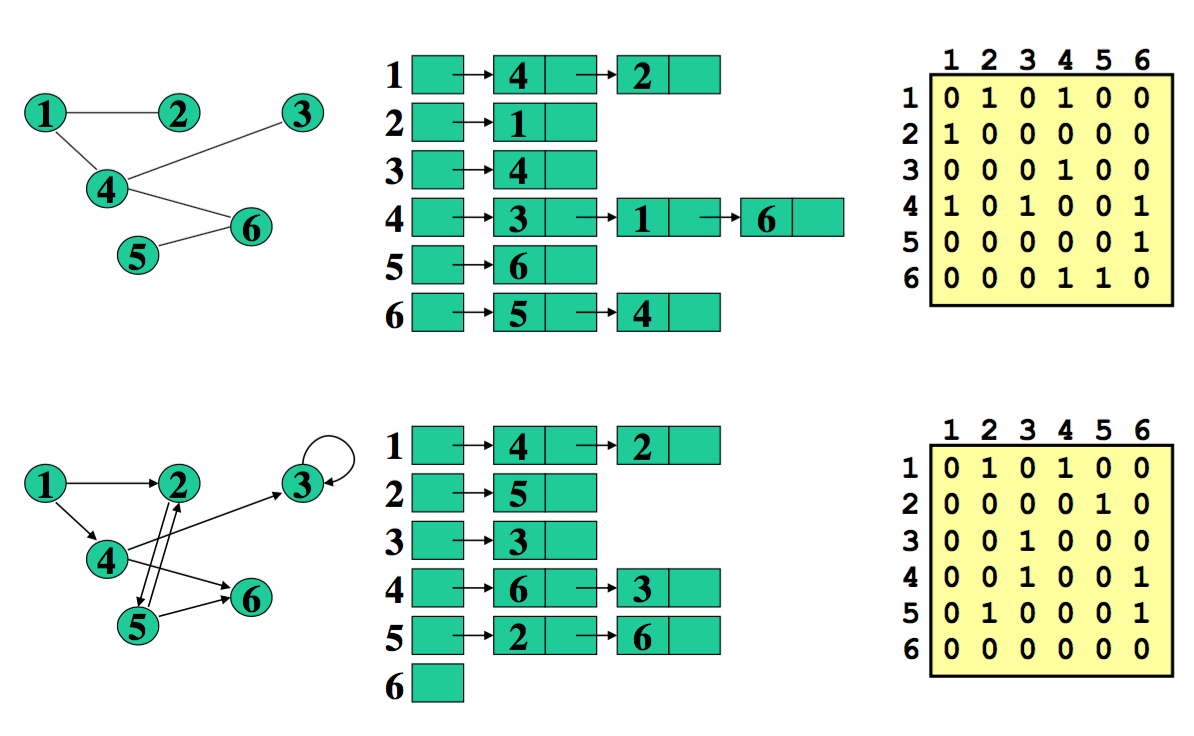
\includegraphics[width=0.75\textwidth]{./notes/immagini/l2-rappr.png}
\caption{Rappresentazione dei grafi}
\end{figure}

\subsubsection{~Lista delle adiacenze}\label{lista-delle-adiacenze}

Per ogni vertice del grafo viene tenuta in memoria una lista \textit{Adj} dei vertici
adiacenti al vertice:

$$
Adj[u] = \{v | uv \in E\} \: \forall u \in V 
$$

Questa rappresentazione richiede memoria per:

\begin{itemize}
\tightlist
\item
  \textit{n\ =\ \textbar{}V\textbar{}} puntatori alla cima delle liste
\item
  \textit{m\ =\ \textbar{}E\textbar{}} elementi per le liste (in totale)
  se il grafo orientato, se è non orientato è \textit{2m}.
\end{itemize}

\subsubsection{Matrice delle adiacenze}\label{matrice-delle-adiacenze}

Viene utilizzata una matrice booleana quadrata che tante righe e tante
colonne, quanti sono i vertici del grafo.

Ogni elemento della matrice vale 1 se i due vertici sono adiacenti, 0
altrimenti:

$$
a_{u,v} = 1 \text{ se } uv \in E
$$

Se il grafo è non orientato, la matrice delle adiacenze è simmetrica.

Il consumo di memoria è $n^2$.

Se il grafo è \textbf{sparso}, ovvero il grado dei vertici è minore del
logaritmo del numero dei vertici, la matrice delle adiacenze risulta
peggiore della rappresentazione con liste in termini di memoria
occupata.

Più formalmente, assumendo che il grafo abbia \textit{n} vertici e \textit{m} archi e che, sia i puntatori, sia gli interi, occupino 32 bit.

Si ha che la lista delle adiacenze occupa $32(n+2m)$, mentre la matrice richiede $n^2$.

La matrice risulta quindi vantaggiosa quando:

\begin{align*}
	32(n+2m) &< n^2 \\
	m &< \frac{n(n-32)}{64}
\end{align*}


\subsection{Calcolo del grafo trasposto}\label{calcolo-del-grafo-trasposto}

Dato un grafo orientato \emph{G=(V,E)} si vuole ottenere $ G^T = (V, E^T)$ in modo che gli archi siano rovesciati, ovvero $E^T = \{uv | vu \in E\}$.

Utilizzando la rappresentazione con la matrice delle adiacenze, è
necessario attraversare metà della matrice e mettere a 1 la cella
\emph{i,j} se \emph{j,i} è a 1. La complessità risulta quindi essere
$O(n^2)$.

Con la lista delle adiacenze l'algoritmo risulta essere


\begin{algorithm}
	\begin{algorithmic}[1]
		\Function{Trasponi}{$Adj,\: Adj^T,\: n$}
			\For{$v = 1 \: to \: n$}
				\State $Adj^T[v] \gets nil$
			\EndFor
			\For{$u = 1 \: to \: n$}
				\State {$x \gets Adj[u]$}
				\While{$x \neq nil$}
					\State{$v \gets x.v$}
					\State{$y \gets nodo(u, Adj^T[v])$}
					\State{$Adj^T[v] \gets y$}
				\EndWhile
			\EndFor
		\EndFunction
	\end{algorithmic}
	\caption{Trasponi: calcolo del grafo trasposto utilizzando la rappresentazione con la lista delle adiacenze}
\end{algorithm}

Ovvero viene attraversata la lista delle adiacenze del grafo originale,
e per ogni elemento delle liste, lo aggiunge ``\emph{al contrario}''
nella nuova lista delle adiacenze.

La complessità risulta quindi essere \emph{O(m+n)}, questo perché il
secondo \texttt{for} esamina tutti i possibili archi, quindi anziché
avere complessità \emph{n} (numero di vertici) ha complessità \emph{m}
(numero di archi).

\subsection{(Esercizio) Ricerca del pozzo
universale}\label{esericizio-ricerca-del-pozzo-universale}

Un vertice è un \textbf{pozzo universale} se può essere raggiunto da
tutti gli altri vertici del grafo, dal quale però non è possibile
raggiungere altri vertici.

Trovare un algoritmo che riesce a risolvere il problema in \emph{O(n)}.


\begin{verbatim}
	- Si cerca un arco tra il nodo 2 -> 1
		- se il bit è a 1, 2 non è un pozzo universale
		- si passa al successivo fino a che non si trova uno nodo che va verso 1,  ad esempio 4->1 a 0
			- in questo modo è possibile escludere il nodo 1
		- in questo modo posso partire dal k+1 in questo caso 5
			- 6->5
				se 0, escludo il 5
				se 1, escludo il 6
		- questo si ripete fino a che non rimane almeno un candidato pozzo
		- Se non c'è nessun canditato, non può esserci un pozzo
		- Se c'è un candidato è necessario verificare che sia un pozzo (forse)
		  la complessità è quindi O(n+n)
\end{verbatim}
% !TEX encoding = UTF-8
% !TEX program = pdflatex
% !TEX root = InformationRetrieval.tex
% !TEX spellcheck = it-IT

% 6 Ottobre 2016

%\chapter{Rappresentazione dei documenti}
%\section{Analisi automatica del testo}

Tutto è iniziato quando George K. \textbf{Zipf}, uno studioso americano di linguistica ha formulato delle leggi empiriche che mettono in relazione la \textbf{frequenza di una parola} con la sua \textbf{forma} e \textbf{significato}. 
Solo in un secondo momento queste leggi sono state applicate all'indicizzazione dei documenti.

L'osservazione di partenza è stata quella che ci sono poche parole che sono veramente molto frequenti, come gli articoli, e che sono poco significative rispetto il contenuto informativo del documento. Ci sono poi tante parole poco frequenti, alcune delle quali sono fortemente correlate al contenuto informativo del documento. Il gioco è quindi quello di sfruttare al meglio tali parole.

Questo andamento può essere rappresentato graficamente, prima andando a contare le frequenze delle singole parole, per poi andare ad ordinarle da quella più frequente a quella meno frequente. La distribuzione così ottenuta è intera, ma può essere approssimata da un'iperbole.

Tipicamente in inglese:
\begin{itemize}
	\item Le due parole più frequenti sono \textit{the} e \textit{of}, mediamente sono il 10\% delle parole del documento.
	\item Le 6 parole più frequenti corrispondo a circa il 20\% delle occorrente e le 50 parole più frequenti corrispondo a circa il 40\% dei testi. Questo deriva dal fatto che la lingua deve essere ridondante in modo che sia facile da capire.
	\item Considerando un'insieme di documenti molto ampio, circa la metà delle singole parole di quel campione compare una sola volta. Queste sono parole più significative dal punto di vista dell'informazione. Tuttavia è necessario tenere conto che in questo insieme di parole possono comparire anche gli errori di battitura.
\end{itemize}

\subsection{Legge di Zipf}

La legge di Zipf afferma che dato un campione di testi e calcolata la frequenza $f$ delle parole, una volta che si sono messe le parole in ordine decrescente di frequenza, cioè si sono ordinate le parole in base al ragno \textit{r}, la distribuzione che si ottiene ha un andamento assimilabile ad una iperbole e si ha che

$$
r \times f = k
$$

ovvero la distribuzione è data da $ f = \cfrac{k}{r}$.

Se anziché ragionare in termini di frequenza assoluta si passa a considerare quella relativa, ovvero la probabilità osservata di occorrenza della parola, la legge di Zipf può essere riscritta come 

$$
r \times P_r = c
$$

Dove $P_r$ è la probabilità di occorrenza della parola che occupa il rango $r$-esimo e $c$ è una costante ($c = 0.1$ per l'inglese).

Si ha che per la lingua inglese $c \approx 0,1$ e l'iperbole che si ottiene è riportata in figura \ref{fig:zipf}

\begin{figure}[htbp]
\centering
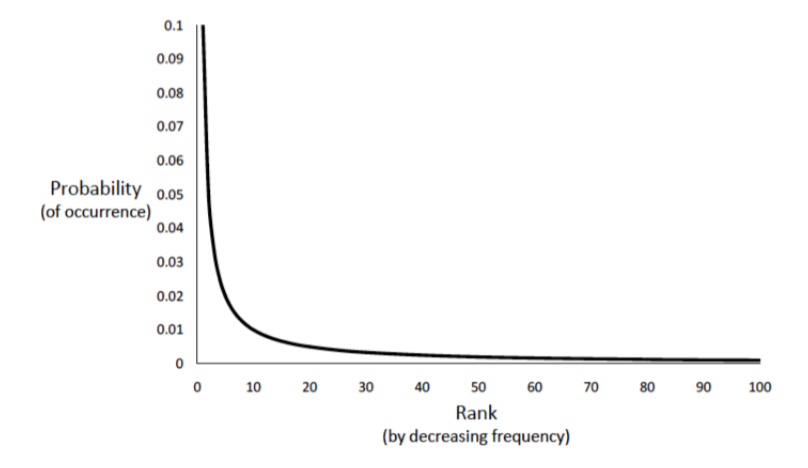
\includegraphics[width=0.55\linewidth]{images/l3-zipf}
\caption{Rango rispetto la probabilità di occorrenza assumendo valida la legge di Zipf con $c = 0.1$}\label{fig:zipf}
\end{figure}

\subsection{Indicazioni di H.P. Luhn}

L'idea per l'indicizzazione è quindi quella di definire due soglie di \textit{cut-off} per evitare di prendere in considerazione le parole troppo frequenti, perché poco significative, e quelle troppo poco, per limitare l'effetto degli errori di battitura.

Ogni parola ha un certo \textbf{resolving power}, ovvero una certa capacità di discriminare il contenuto del documento da quello degli altri e di caratterizzare il contenuto della collezione.

\begin{figure}[htbp]
	\centering
	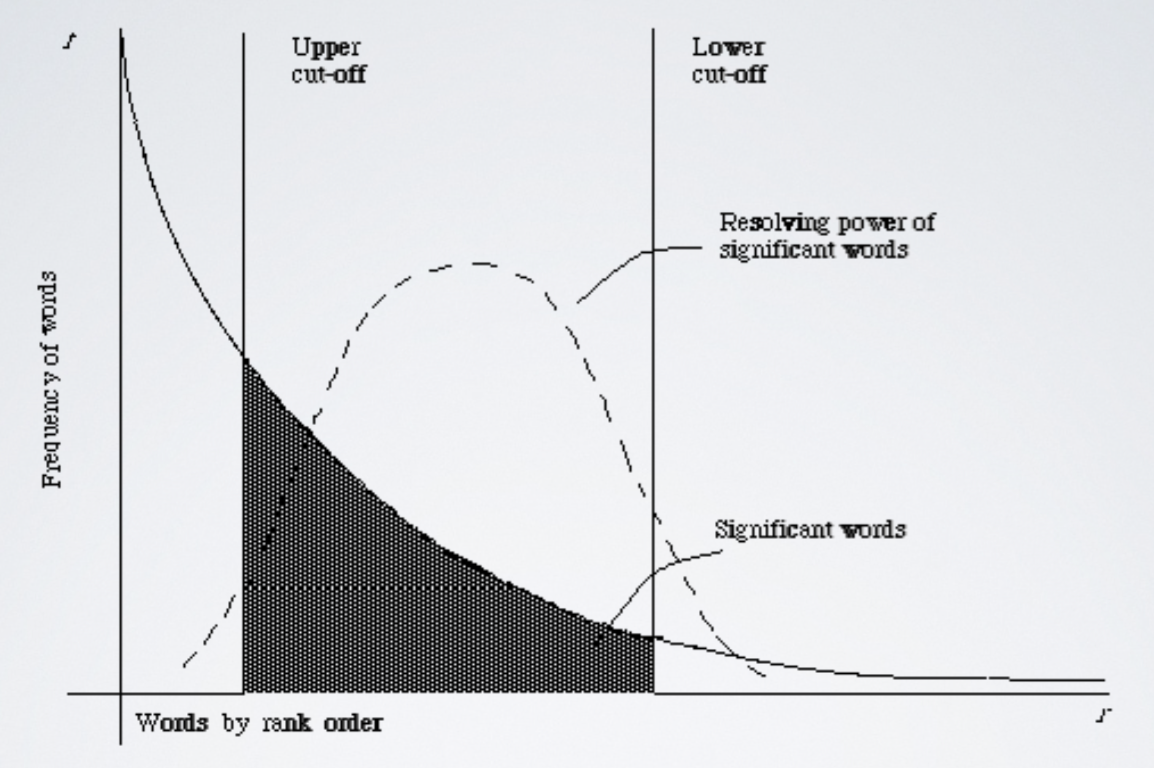
\includegraphics[width=0.55\linewidth]{images/l3-cutoff}
	\caption{Plot della curva $r \times f$ che evidenzia la posizione delle parole significative.}
\end{figure}

Questo vale per le collezioni generiche dei documenti, mentre se si parla di un argomento specifico si può dare maggiore peso a determinate parole. Ad esempio può capitare in che se viene preso in esame un manuale di MySQL è ovvio che le parole ``MySQL'' e  ``table'' compariranno tante volte anche se non sono articoli.

C'è anche un altro discorso relativo alla forma plurale, che in conteggio di frequenza vengono considerate come diverse, quando in realtà può essere che abbia lo stesso valore informativo della forma singolare. In alcuni casi è quindi opportuno sommare le occorrenze della forma plurale e di quella singolare.

Si ha quindi che i passi per applicare le indicazioni di Luhn sono:

\begin{itemize}
	\item Si calcoli la frequenza di ogni descrittore in ogni documento della collezione di riferimento. C'è inoltre da scegliere come trattare le parti di contorno dei documenti come l'indice, la premessa, ecc. tali parti tipicamente non vengono considerate.
	\item Si calcoli la frequenza totale di ogni descrittore.
	\item Si ordino i descrittori per frequenza decrescente.
	\item Si scelga una soglia di \textit{upper cut-off} e si rimuovano dalla lista i descrittori con frequenza superiore alla soglia. In questo modo si rimuovono gli articoli, le preposizioni, ecc.
	\item Si scelga un'altra soglia di \textit{lower cut-off} e si rimuovano dalla lista i descrittori con frequenza inferiore al valore di soglia. In questo modo si rimuovono i descrittori ``rumore''  o che non apportano alcun contribuito alla descrizione del contenuto.
\end{itemize}

\noindent Entrambe le soglie possono essere calcolate in modo euristico.

Le parole che vengo eliminate dalle soglie di cut-off vengono nominate \textbf{stop word} e sono raccolte nella lista che prende il nome di \textbf{stop list}.


\textbf{{\color{Red} Possibile esercizio:}} Domande relative alle osservazioni proposte da Zipf e Luhn.

\section{Indicizzazione}

L'indicizzazione ha l'obiettivo di rappresentare il contenuto informativo di un documento e nel tempo questo processo ha preso una struttura a fasi.

Il documento viene rappresentato da dei descrittori che vengono utilizzati per la costruzione degli indici, utili al reperimento dell'informazione.

Quindi l'indicizzazione fornisce automaticamente una rappresentazione più compatta e direttamente utilizzabile del contenuto informativo del documento. Gli indici sono utilizzati come surrogati del contenuto del documento durante la fase di reperimento.

L'indicizzazione può essere svolta:
\begin{itemize}
	\item manualmente
	\item in modo automatico
	\item in modo semi-automatico, quando è necessario intervenire all'interno del processo per prendere delle decisioni che non possono essere prese in modo automatico.
\end{itemize}

\noindent Tutti questi metodi funzionano estraendo direttamente dal documento le informazioni. Tuttavia possono essere estesi in modo che vengano presi in considerazione anche dei dizionari o delle meta-informazioni.

\begin{figure}[htbp]
	\centering
	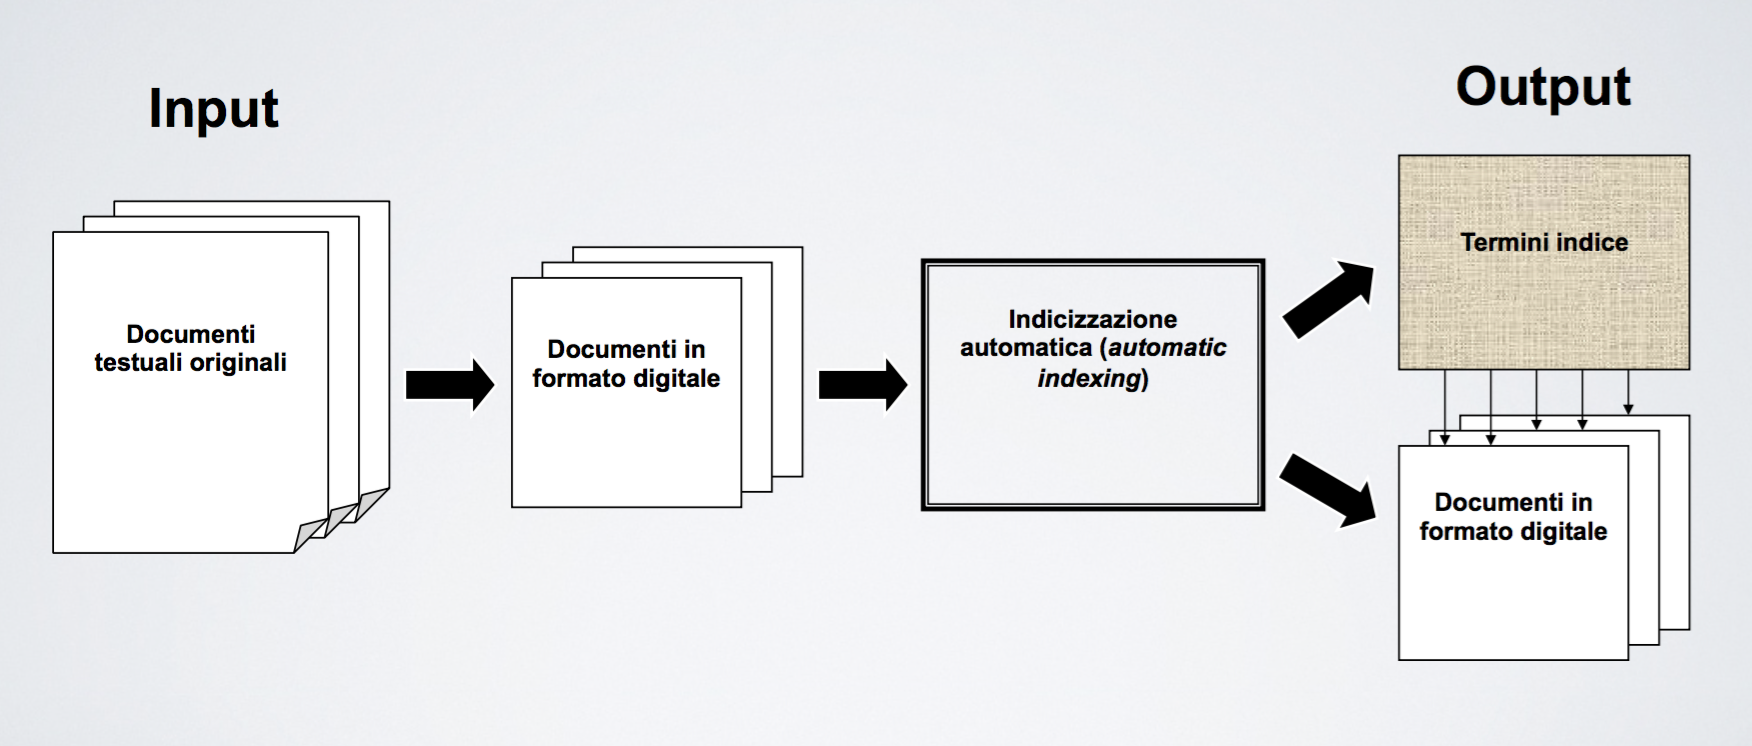
\includegraphics[width=0.7\linewidth]{images/l3-indicizzazione}
	\caption{Schema generale dell'indicizzazione}
\end{figure}

\subsection{Indicizzazione automatica dei testi}

L'indicizzazione automatica di un documento testuale è un processo che esamina automaticamente gli oggetti informativi (parole, frasi, didascalie, figure, ecc.) che compongono il documento e produce una lista di termini indice presenti nell'intera collezione dei documenti.

L'estrazione dei termini indice viene fatta da appositi algoritmi e, una volta estratti, questi vengono collegati ai diversi documenti che li contengono.
Così facendo durante il reperimento sarà sufficiente fare riferimento ai termini indice e non all'intera collezione.

\subsection{Attuazione dell'indicizzazione automatica}

L'indicizzazione automatica dei documenti testuali viene eseguita in più fasi, che devono essere attuate in sequenza:

\begin{enumerate}
	\item Analisi lessicale e selezione delle parole.
	\item Eventuale rimozione delle stop word.
	\item Riduzione delle parole originali alle rispettive radici (\textit{STEM}). Ad esempio le forme plurali vengono ridotte a quelle singolari.
	\item Composizione dei termini. Come ad esempio ``information retrieval''. Ovvero le parole vengono combinate tra loro quando si trovano ad una determinata distanza.
	\item Creazione dell'indice.
	\item Eventuale pesatura degli elementi dell'indice. 
\end{enumerate}

Alla fine di queste fasi l'indice sarà composto da parole, termini e frasi che noi riteniamo significative, assieme alle informazioni del peso che gli diamo e alla loro frequenza all'interno dei documenti.









\subsubsection{Errori possibili}\label{errori-possibili}

Con la formulazione delle due ipotesi è possibile commettere due tipi di
errori:

\begin{itemize}
\item
  \textbf{errore di primo tipo}: viene rifiutata $ H_0 $ quando questa è
  vera.
\item
  \textbf{errore di secondo tipo}: viene accettata $ H_0 $ quando $ H_0 $ è falsa.
\end{itemize}

Per come è stato costruito il test statistico si ha che

$$
P(\text{errore 1° tipo}) = 1 - P(\text{accettare } H_0 \text{ quando è vera})
$$

e viene fissato ad $\alpha$, perché

$$ P(\text{accettare } H_0 \text{ quando è vera}) = 1- \alpha $$

Tuttavia non viene detto nulla a riguardo dell'errore del secondo tipo.
Si sa solo che non si possono minimizzare i due errori
contemporaneamente, perché sono tra loro correlati.

Ma alla fine quello che conta è l'errore di primo tipo, perché la
domanda che ci si pone è ``\emph{A:i dati sperimentali sono compatibili
con $ H_0 $?}'' piuttosto che ``\emph{B:Quale tra $ H_0 $ e $ H_1 $ è vera?}''.

L'approccio adottato prevede quindi di fissare l'errore più importante
(con $\alpha$) e minimizzare la probabilità d'errore del secondo
tipo.

Sfruttando i dati è comunque possibile ridurre entrambi i tipi d'errore
perché se il numero \emph{n} di dati a disposizione è grande e quanto
più è dispersa la variabile esplicativa, tanto più gli errori commessi
sono minori.

\subsection{Rilassando le ipotesi}\label{commenti}

Finora è stato assunto che i dati seguano una distribuzione normale,
quindi prima di effettuare una regressione lineare è necessario andare a
verificare che questo sia vero.

Per effettuare questa verifica servono delle tecniche grafiche ed
analitiche complesse, pertanto è più ragionevole utilizzare un approccio
alternativo che verifica a posteriori la normalità dei dati.

Un'altra ipotesi fatta riguarda la conoscenza della varianze delle
distribuzione, ma nel lato pratico questo è un parametro ignoto.

Utilizzando il metodo dei minimi quadrati è possibile solamente stimare
i coefficienti $\beta$ e non la varianza.

Tuttavia, considerando $y = \beta_0 + \beta_1x + \epsilon$, si può
isolare $\epsilon$ e stimarlo utilizzando i residui osservati:

\begin{align*}
	\hat{\epsilon}_i  &= r_i \\ 
								&= y_i - \hat{y}_i = \\
								  &= y_i - \hat{\beta}_0 - \hat{\beta}_1x_i
\end{align*}


Si può quindi costruire uno stimatore per la varianza della componente di
errore utilizzando la varianza dei residui\footnote{La media dei residui è 0.} che è facilmente calcolabile.

\begin{align*} 
	\hat{\sigma}^2 &= \frac{1}{n}\sum\limits_{i=1}^n (r_{i} - 0)^2\\
								&= \frac{1}{n}\sum\limits_{i=1}^n (y_i - \hat{\beta}_0 - \hat{\beta}_1x_i)^2
\end{align*}

Utilizzando questo stimatore si tende ad ottenere \textbf{una sottostima} della varianza, pertanto conviene utilizzare

\begin{align*} 
\hat{s}^2 &= \frac{1}{n-2}\sum\limits_{i=1}^n (r_{i} - 0)^2\\
				 &= \frac{1}{n-2}\sum\limits_{i=1}^n (y_i - \hat{\beta}_0 - \hat{\beta}_1x_i)^2
\end{align*}

\subsubsection{Il problema di verifica delle ipotesi senza $\sigma^2$}\label{il-problema-di-verifica-delle-ipotesi-senza-sigma2}

Dal momento che non è nota la varianza, non è più possibile utilizzare $ z $ per effettuare la verifica dell'ipotesi su $ \beta_1 $, ma è necessario utilizzare un'altra statistica test:

$$
t_{oss} = \frac{(\hat{\beta}_1 - 0)}{\sqrt{\frac{s^2}{\sum_{i=1}^{n} (x_i - \bar{x})^2}}}
$$

Il pedice \textit{oss} indica che viene influenzata dai dati osservati.

Il funzionamento di $ t_{oss} $ è analogo a quello di $ z $: se $ H_0 $ è vera ci si aspetta che $ t_{oss} $ assuma valori vicini allo 0, mentre se è vera $ H_1 $ ci aspettiamo che assuma valori lontani dallo 0.

Per determinare il valore di $ t_{oss} $ non è possibile utilizzare la distribuzione normale, perché la varianza non è nota, ed è quindi necessario utilizzare la \textbf{\textit{t} di Student}\footnote{Questo è possibile perché nelle nostre ipotesi gli errori seguono la distribuzione normale e sono tra loro indipendenti.}.

La distribuzione \emph{t di Student} dipende da un solo parametro che
prende il nome di \textbf{gradi di libertà}. Durante a verifica
dell'ipotesi sul coefficiente angolare della retta di regressione, il
grado di libertà è \emph{n-2}, ovvero è stato dimostrato che:

$$
t_{oss} \approx t \text{ di Student con } n - 2 \text{ gradi di libertà.}
$$

Il grafico di questa distribuzione è simile a quello della normale, solo
che ha delle code più pesanti.

\begin{figure}[htbp]
\centering
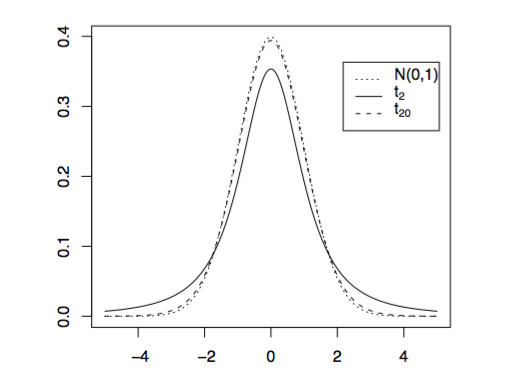
\includegraphics{./notes/immagini/l6-fig5.png}
\caption{Confronto della $ t $ di Student con la normale $ \mathcal{N}(0,1) $}
\end{figure}

In questo caso però non conviene utilizzare un confronto sulla soglia dei valori, perché questo potrebbe enfatizzare troppo delle differenze minime, portando a dei valori completamente diversi.

L'idea è quindi quello di utilizzare il \textbf{livello di significatività osservato} o \textbf{p-value}, un indicatore uguale alla probabilità di osservare, supponendo vera $ H_0 $, un valore di $ t_{oss} $ uguale o ``più lontano'' da $ H_0 $ di quanto effettivamente è osservato, ovvero costituisce una misura di quanto l'ipotesi nulla è plausibile sulla base dei dati.

Cosa \textbf{NON} è il \textit{p-value}:
\begin{itemize}
	\item \textbf{Non} è la probabilità che l'ipotesi nulla sia vera o falsa. Non è connessa a nessuna delle due.
	\item \textbf{Non} è la probabilità che un'osservazione sia un caso.
	\item \textbf{Non} è la probabilità di rifiutare $ H_0 $ quando questa è vera
	\item \textbf{Non} è la probabilità di ottenere lo stesso risultato replicando l'esperimento.
\end{itemize}


\begin{figure}[htbp]
\centering
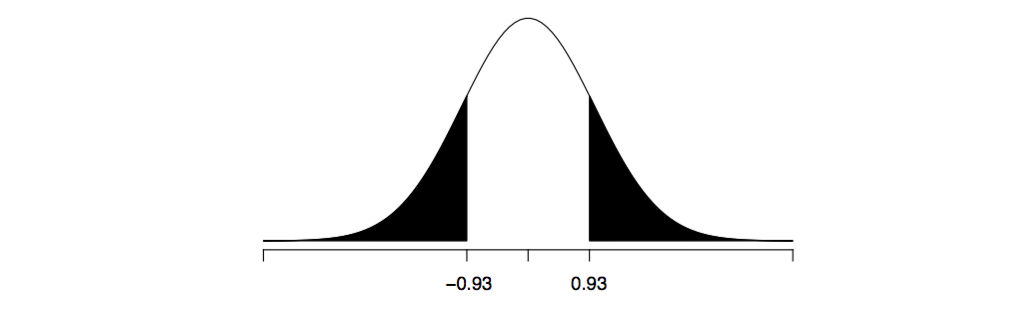
\includegraphics[width=.9\textwidth]{./notes/immagini/l6-fig7.png}
\caption{La curva mostra la densità di una \textit{t} di Student con $ t_{oss} = 0.93 $. Poiché lontano da 0 vuol dire lontano da $ H_0 $, l'area annerita fornisce una approssimazione della probabilità di osservare, quando è vera $ H_0 $, un valore più lontano dall'ipotesi nulla rispetto a quanto osservato.}
\end{figure}


Questo livello varia da 0 a 1 e più è grande, più i dati sono vicini ad $ H_0 $.

\begin{itemize}
\item
  Se vale 0 (o è inferiore ad $ \alpha $) vuol dire che sotto $ H_0 $ non è possibile osservare nessun
  altro valore più lontano da $ H_0 $, ovvero il valore osservato per $ t_{oss} $
  è uno dei più lontani possibili. L'evidenza empirica è fortemente contraria all'ipotesi nulla che quindi va rifiutata.
\item
  Se vale 1 (o è maggiore di $ \alpha $) vuol dire che sotto $ H_0 $ tutti i possibili valori osservabili
  per $ t_{oss} $ sono ``non più vicini di quello osservato'', ovvero quello
  osservato è uno dei più vicini possibili. L'evidenza empirica non è sufficientemente contraria all'ipotesi nulla, la quale non può essere rifiutata.
\end{itemize}

\emph{lontano da $ H_0 $} equivale a dire \emph{``lontano da 0 in entrambe le
direzione''} quindi, nel caso delle vendite ($ t_oss = 9.921 $):

\begin{align*}
\text{livello di significatività osserato } &= P(|t \text{ con 198 gradi}| \geq t_{oss}) \\
																	&= P(|t \text{ con 198 gradi}| \geq 9.921) \\
														           &= 2xP(t \text{ con 198 gradi} \geq 9.921)
\end{align*}

\begin{figure}[htbp]
	\centering
	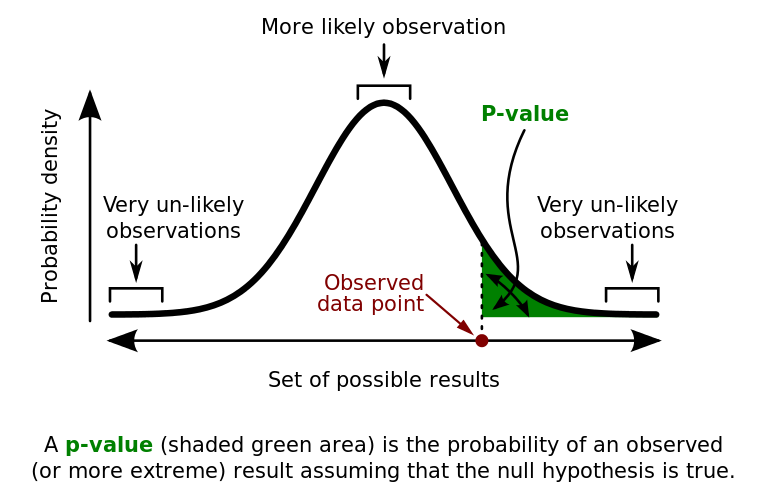
\includegraphics[width=.7\textwidth]{./notes/immagini/l6-fig7-1.png}
\end{figure}

Il calcolo della probabilità viene poi fatto utilizzando una tabella o
un software apposito. Nell'esempio si ha che il livello di significatività osservato è 0.

Ovvero, se la spesa in pubblicità via radio ha un effetto sulle vendite allora noi ci aspetteremo valori ``Più lontani da $ H_0 $ di quanto
osservato''.

Il che vuol dire che il valore osservato di $ t_{oss} $ è molto strano (poco plausibile) quando $ H_0 $ è vera.

\paragraph{Interpretazione alternativa del \textit{p-value}} Supponendo di formare tutti i possibili campioni di 200 elementi e di calcolare $ t_{oss} $ per ognuno di questi. Allora il \textit{p-value} è la percentuale di valori di $ t_{oss} $ maggiori di 9.921\footnote{Valore di $ t_{oss} $ calcolato per il data set d'esempio delle slide}, che per quanto calcolato prima ci si aspetta che sia 0. Ma allora 9.921 è un valore che difficilmente può capitare quando $ H_0 $ è vera, e quindi i dati smentiscono l'ipotesi nulla, che è da rifiutare.

La procedura per accettare o rifiutare l'ipotesi è riportata in Figura \ref{pvalueacc}.

\begin{figure}[htbp]
\centering
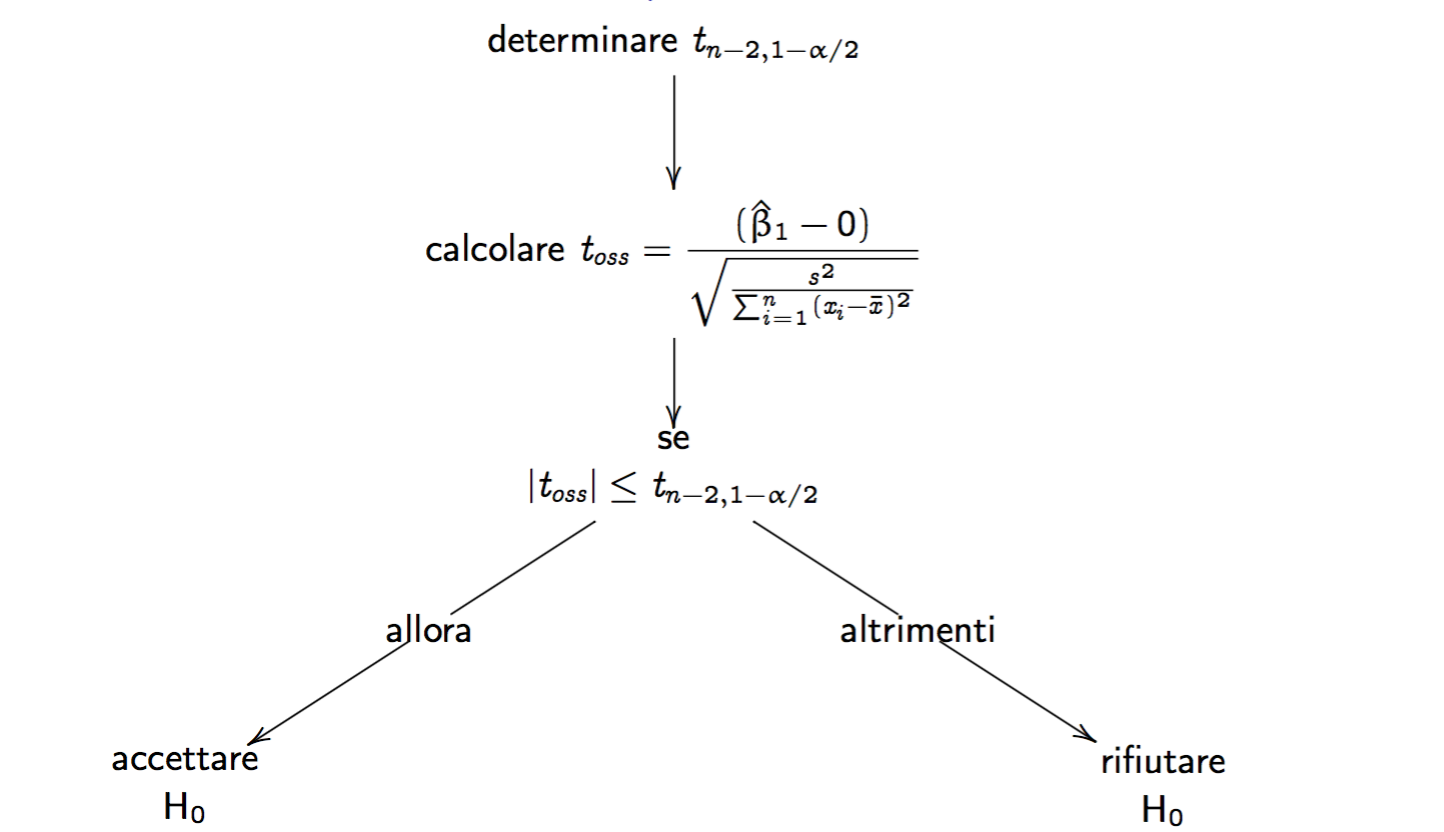
\includegraphics[width=.9\textwidth]{./notes/immagini/l6-fig9-1.png}
\caption{Regola per l'accettazione o il rifiuto di $ H_0 $. $ t_{g,p} $ indica il percentile $ p $-esimo di una \textit{t} di Student con \textit{g} gradi di libertà. L'albero fornisce una regola che garantisce di accettare $ H_0 $ quando questa è vera con probabilità $ 1 - \alpha $.}\label{pvalueacc}
\end{figure}

\subsubsection{Intervallo di confidenza}\label{intevallo-di-confidenza}
In modo analogo a come è stato fatto nel caso di $ \sigma^2 $ noto è possibile definire un'intervallo di confidenza per la stima.

$$
P\Bigg( -t_{n-2, 1-\alpha/2} \leq \frac{(\hat{\beta}_1 - \beta_1)}{\sqrt{\frac{s^2}{\sum_{i=i}^{n} (x_i - \bar{x})^2}}}\leq  t_{n-2, 1-\alpha/2}\Bigg) = 1 - \alpha
$$

Da cui si deriva che:\todo[inline]{Nelle slide non c'è il termine $ t_{n-2, 1-\alpha/2} $ ma secondo me è un errore non metterlo}

$$
\Bigg[ \hat{\beta}_1 - t_{n-2, 1-\alpha/2}  \sqrt{\frac{s^2}{\sum_{i=i}^{n} (x_i - \bar{x})^2}} \:,\: \hat{\beta}_1 + t_{n-2, 1-\alpha/2} \sqrt{\frac{s^2}{\sum_{i=i}^{n} (x_i - \bar{x})^2}}  \Bigg]
$$

\subsection{Verifica di ipotesi su $ \beta_0 $}\label{verifica-di-ipotesi-su-beta0}

In modo simile è possibile stimare $ \beta_0 $, anche se risulta molto meno
interessante, perché è $ \beta_1 $ che fornisce la relazione tra le \emph{x} e
le \emph{y}.

Come prima cosa è necessario stimare la varianza di $ \hat{\beta}_0 $:

$$
Var(\hat{\beta}_0) = \frac{\sum_{i=1}^{n} x_{i}^2}{n \sum_{i=1}^{n} (x_i - \bar{x})^2}s^2
$$

Le ipotesi diventano

$$
\begin{cases}
H_0 : \beta_0 = \beta' \\
H_1 : \beta_0 \neq \beta' 
\end{cases}
$$

dove $ \beta' $ è un valore fissato, ad esempio 0.

La statistica test diventa quindi:

$$
t_{oss}  = (\hat{\beta}_0 - \beta') \Bigg/ s \sqrt{\frac{\sum_{i=1}^{n} x_{i}^2}{n \sum_{i=1}^{n} (x_i - \bar{x})^2}}
$$

con intervallo di confidenza definito da

$$
\Bigg[ \hat{\beta}_0 - t_{n-2, 1-\alpha/2} s \sqrt{\frac{\sum_{i=1}^{n} x_{i}^2}{n \sum_{i=1}^{n} (x_i - \bar{x})^2}} \:,\: \hat{\beta}_0 + t_{n-2, 1-\alpha/2} s \sqrt{\frac{\sum_{i=1}^{n} x_{i}^2}{n \sum_{i=1}^{n} (x_i - \bar{x})^2}}\Bigg]
$$

Da notare che in questo modo non viene definito un intervallo di confidenza simultaneo, ovvero che vale sia per $ \beta_0 $ che per $ \beta_1 $.


\subsection{Verifica di ipotesi globale sul modello}\label{verifica-di-ipotesi-globale-sul-modello}

Per misurare la varianza spiegata dal modello abbiamo il coefficiente di
determinazione $R^2$ che misura la varianza spiegata dal modello
rispetto a quella complessiva. Non abbiamo però un criterio per capire
se l'$R^{2}$ osservato è grande o piccolo.

Anche in questo caso è possibile impostare un problema di verifica di
ipotesi, l'ipotesi nulla sarà l'indipendenza lineare tra \emph{x} e
\emph{y}, mentre l'ipotesi alternativa prevederà che la retta spieghi,
almeno in parte, la relazione presente.

Generalmente la statistica test più utilizzata per questo problema è:

$$
F_{oss} = \frac{\frac{R^2}{k -1}}{\frac{1-R^2}{n-k}} = \Bigg( \frac{R^2}{1-R^2} \Bigg) \Bigg( \frac{n-k}{k-1}\Bigg)
$$

dove \textit{k} rappresenta il numero di parametri utilizzati nel modello, nel nostro caso 2.

La statistica $ F_{oss}  $ può essere anche vista come il rapporto tra la media dei quadrati degli scarti spiegati dal modello e la corrispondente media dei quadrati degli scarti residui, pertanto ci aspettiamo $ F_{oss}  $ grande quando $ H_0 $ è falsa.

Nelle ipotesi di normalità ed indipendenza degli errori, si ha che $ F_{oss} $ si distribuisce come una variabile aleatoria detta \textbf{\textit{F} di Snedecor} con $ k-1 $ gradi di libertà al numeratore e $ n-k $ gradi di libertà al denominatore.

Il valore $ F_{oss} $ deve essere quindi confrontato con la \textit{F} di Snedecor utilizzando una tavola dei percentili o con un apposito software. Maggiore è $ F_{oss} $, minore è la probabilità che $ H_0 $ sia vera.

Ad esempio, con $ F_{oss}  = 98.42 $ si ha che il valore osservato è molto più grande del quantile $ 0.999 (\text{che vale circa } 11.15)$, sia ha quindi che la probabilità di osservare un valore uguale o più lontano da $ H_0 $ rispetto a quando osservato è inferiore di un millesimo.
I dati suggeriscono quindi che nel campione osservato si presenta una dipendenza lineare tra \textit{x} e \textit{y} e anche che questa dipendenza dovrebbe esserci in tutta la popolazione.

Il livello di significatività osservato fornisce quindi la probabilità di ottene una statistica \textit{F} maggiore o uguale a quella ottenuta dai dati a disposizione nel caso ci sia indipendenza tra \textit{x} e \textit{y}.

Il vantaggio di questo livello è che nasconde tutti i dettagli riguardo la statistica test.

Tipicamente, se il livello di significatività osservato è inferiore a $ 0.01 $ i risultati sono considerati altamente significativi \textbf{contro} $ H_0 $, mentre se risulta compreso tra $ 0.01 $ e $ 0.05 $ i risultati sono comunque significativi contro $ H_0 $, ovvero è molto probabile che $ H_0 $ sia falsa.

Viceversa, se risulta maggiore di $ 0.1 $ si conclude che i dati non contengono elementi tali da poter rifiutare $ H_0 $ e quindi sono \textbf{non significativi}.

\section{Effettuare previsioni}\label{effettuare-previsioni}

Una volta fatto il modello, è carino utilizzarlo per effettuare delle
previsioni o delle simulazioni sul futuro.

Questo può essere fatto fissando un determinato valore $ x_0 $ e calcolando \textit{y} utilizzando i coefficienti stimati:

$$
\hat{y}_0 = \hat{\beta}_0 + \hat{\beta}_1 x_0
$$

Tuttavia può essere interessante avere anche un intervallo di precisione da associare alla stima $ \hat{y}_0 $.

Partendo dal modello di riferimento si ottiene:

\begin{align*}
	\hat{y}_0 &= \hat{\beta}_0 + \hat{\beta}_1 x_0 + \epsilon \\
					&= (\bar{y} - \hat{\beta}_1 \bar{x}) + \hat{\beta}_1 x_0 + \epsilon \\
					&= \bar{y} + \hat{\beta}_1(x_0 \bar{x}) + \epsilon 
\end{align*}

Si ha quindi che:

\begin{align*}
	Var(\hat{y}_0) &= Var(\bar{y}) + Var(\hat{\beta}_1)(x_0 - \bar{x})^2 + Var(\epsilon) \\
	                         &= \sigma^2 \Bigg( 1 + \frac{1}{n} + \frac{(x_0 - \bar{x})^2}{\sum_{i=1}^{n} (x_i - \bar{x})^2 }\Bigg)
\end{align*}

che può essere stimata utilizzando $ s^2 $ al posto di $ \sigma^2 $

$$
\widehat{Var(\hat{y}_0)} = s^2 \Bigg( 1 + \frac{1}{n} + \frac{(x_0 - \bar{x})^2}{\sum_{i=1}^{n} (x_i - \bar{x})^2} \Bigg)
$$

L'intervallo di precisione risulta quindi essere

$$
\Bigg[ \hat{y}_0 - t_{n-2, 1-\alpha/2}\sqrt{\widehat{Var(\hat{y}_0)}} \:, \:\hat{y}_0 + t_{n-2, 1-\alpha/2}\sqrt{\widehat{Var(\hat{y}_0)}}\Bigg]
$$

Nell'esempio delle vendite, se $ x_0 = 60 $ si ottiene $ y_0 = 21.4614 $ con un intervallo di previsione $ [12.88 \; , \: 30.04] $ valido con il $ 95\% $ di probabilità.

Effettuando il calcolo dell'intervallo per ogni punto del dominio è possibile ottenere un grafico che rappresenta le \textbf{bande di previsione} ottenute.

\begin{figure}[htbp]
\centering
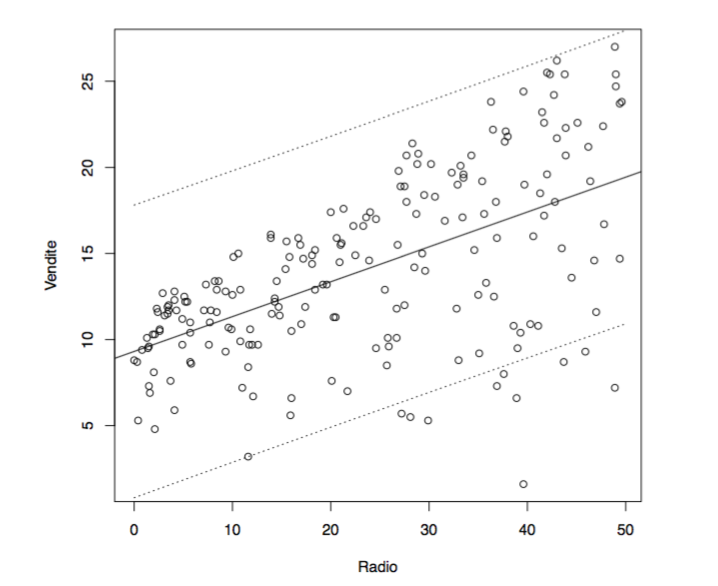
\includegraphics[width=.6\textwidth]{./notes/immagini/l6-fig10-1.png}
\caption{Bande di previsione}
\end{figure}

\subsection{Verifica del modello mediante i residui}

Anche le previsioni sono influenzate dalle ipotesi riguardo la distribuzione degli errori e dalla non variabilità della varianza.
Può succedere che i dati analizzati non soddisfino queste ipotesi ed è necessario avere degli strumenti che permettono di identificare questi casi.

Il modo più semplice per verificare ciò è rappresentare con un grafico, ad esempio con un istogramma, la distribuzione dei residui per osservare se questa ha la classica forma campanulare della distribuzione normale.

\begin{figure}[htbp]
\centering
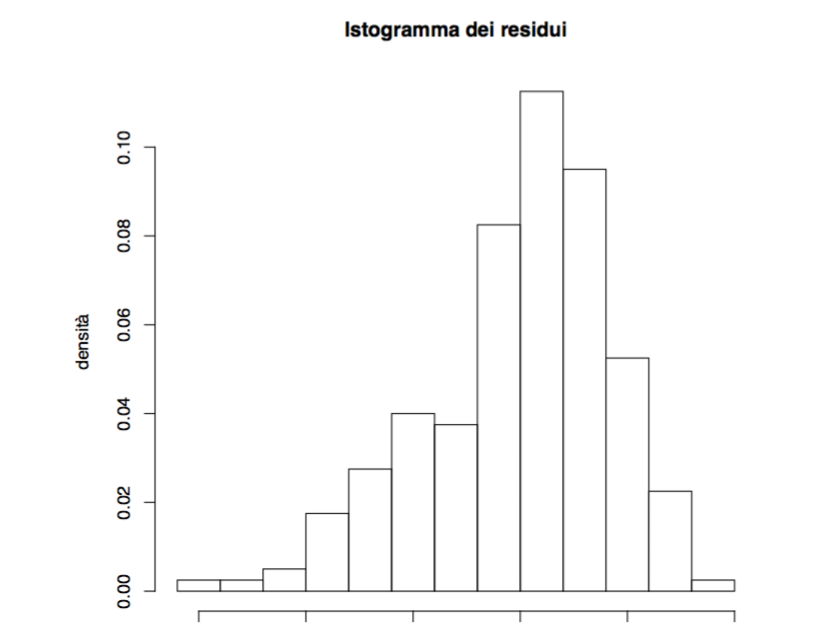
\includegraphics[width=.5\textwidth]{./notes/immagini/l6-fig11-1.png}
\caption{Istogramma dei residui per il data set delle vendite. In questo caso la campana non è proprio centrata, ma questo può essere dovuto a fattori casuali.}
\end{figure}

Un altro grafico è il tracciamento dei residui rispetto la stima $ \hat{y} $ ottenuta il quale aiuta a cogliere alcuni aspetti che ci aspettiamo vengano rappresentati dal modello.

\begin{figure}[htbp]
\centering
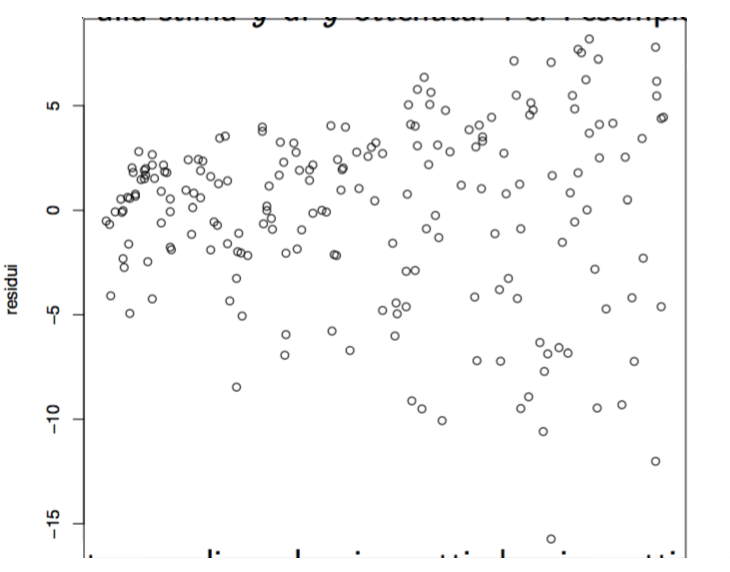
\includegraphics[width=.5\textwidth]{./notes/immagini/l6-fig12-1.png}
\caption{Residui rispetto $ \hat{y} $}
\end{figure}

Alternativamente, è possibile tracciare i residui rispetto alle \textit{x}. In questo modo è possibile osservare se la varianza è costante o se ci sono degli effetti sistematici che il modello non ha colto, oppure se il modello utilizzato non è adeguato.

\begin{figure}[htbp]
	\centering
	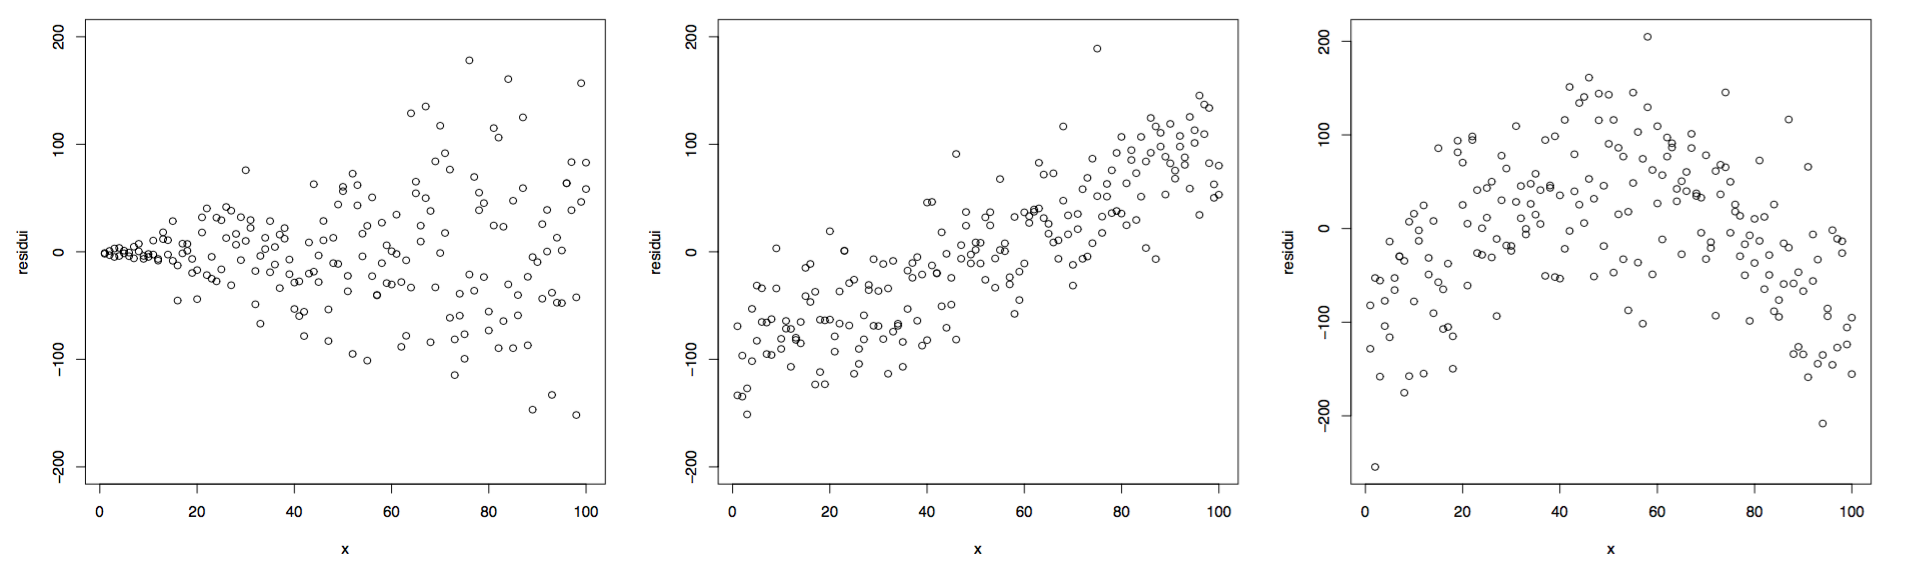
\includegraphics[width=\textwidth]{./notes/immagini/l6-fig13-1.png}
	\caption{Da sinistra verso destra: Varianza non costante, componente sistematica non considerata dal modello, modello inadeguato.}
\end{figure}


Dai grafici è possibile notare anche la presenza di valori anomali (\textbf{outliers}), osservazioni errate che non rispettano la distribuzione, che devono essere trattate in modo particolare per evitare che non influenzino in modo errato il modello.

Per verificare se la distribuzione è normale si può costruire un \textbf{qq-plot}.
Come prima cosa viene creata la distribuzione dei residui per i campioni osservati in modo che ogni punto sia caratterizzato dalla percentuale di punti minori o uguali rispetto alla totalità dei dati. Questa percentuale viene stimata utilizzando le varie frequenze.
Dopodiché è possibile confrontare i quantili della distribuzione ottenuta con quelli della normale standardizzata. Se per ciascuno punto i quantili sono circa uguali a quelli della normale, allora anche la distribuzione dei residui può essere considerata normale.

\begin{figure}[htbp]
	\centering
	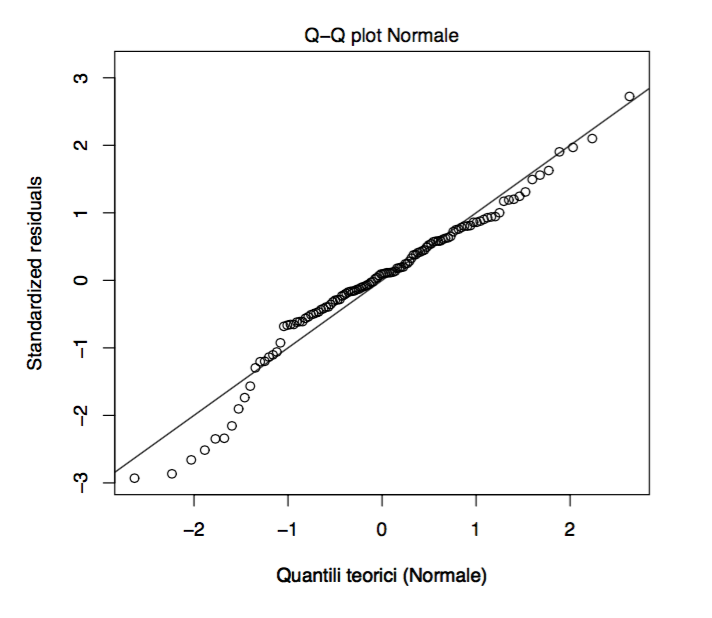
\includegraphics[width=.6\textwidth]{./notes/immagini/l6-fig14-1.png}
	\caption{QQ-Plot, tanto più i punti sono vicini alla bisettrice, tanto più la distribuzione può essere considerata normale.}
\end{figure}




\chapter{Il modello lineare nei parametri}

\textbf{Problema di riferimento:} come il prezzo influenza il consumo di
gas? Si hanno a disposizione le informazioni relative alla domanda di
gas e al prezzo dello stesso per 20 città in Texas.

Si vuole riuscire a capire se c'è una correlazione tra le due cose.

\begin{figure}[htbp]
	\centering
	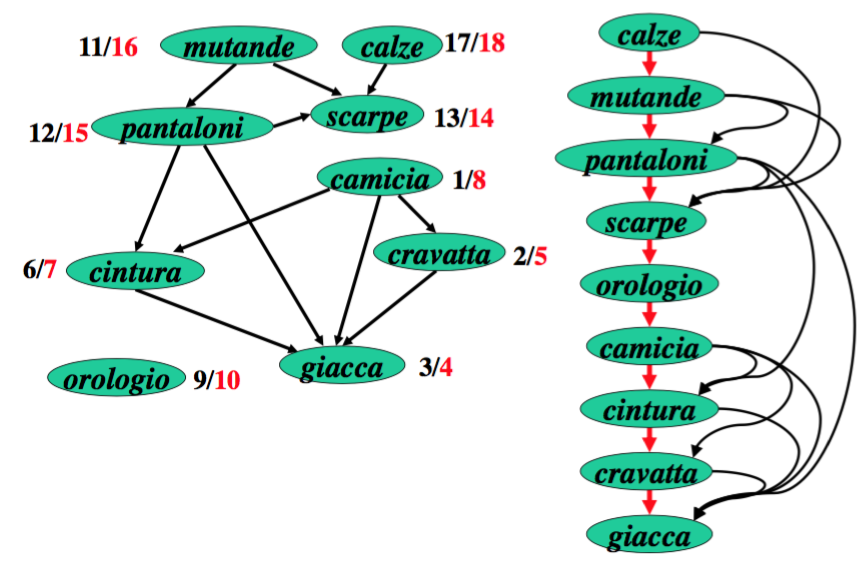
\includegraphics[width=.5\textwidth]{./notes/immagini/l7-fig1.png}
\end{figure}

\section{Un primo modello lineare}\label{un-primo-modello-lineare}

Ipotizzando che ci sia una relazione lineare è possibile utilizzare il
modello del capitolo precedente:

$$
y = \alpha + \beta x + \epsilon
$$

$$
\hat{\beta} = \frac{cov(X,Y)}{var(X)} \qquad \hat{\alpha} = \bar{y} - \hat{\beta}\bar{x}
$$

Utilizzando l'ambiente R si ottengono delle informazioni relative all
modello ottenuto:

\begin{verbatim}
lm(formula = gas ~ prezzo)
Residuals:
    Min      1Q  Median      3Q     Max
-40.625 -10.719  -1.136  14.073  38.292
Coefficients:
            Estimate Std. Error t value Pr(>|t|)
(Intercept)  138.561     13.552  10.225 6.34e-09 ***
prezzo        -1.104      0.202  -5.467 3.42e-05 ***
---
Signif. codes:  0 ‘***’ 0.001 ‘**’ 0.01 ‘*’ 0.05 ‘.’ 0.1 ‘ ’ 1
Residual standard error: 20.86 on 18 degrees of freedom
Multiple R-Squared: 0.6241,     Adjusted R-squared: 0.6033
F-statistic: 29.89 on 1 and 18 DF,  p-value: 3.417e-05
\end{verbatim}

Dai dati si può notare che l'indice $ R^2 $ è uguale a 0.62, il che indica un buon andamento lineare.
Inoltre come \textit{p-value} si ottiene un valore molto basso, il che porta a rifiutare l'ipotesi nulla.

Tracciando però i grafici dei residui è possibile osservare c'è una componente indipendente che non è lineare.

\begin{figure}[htbp]
	\centering
	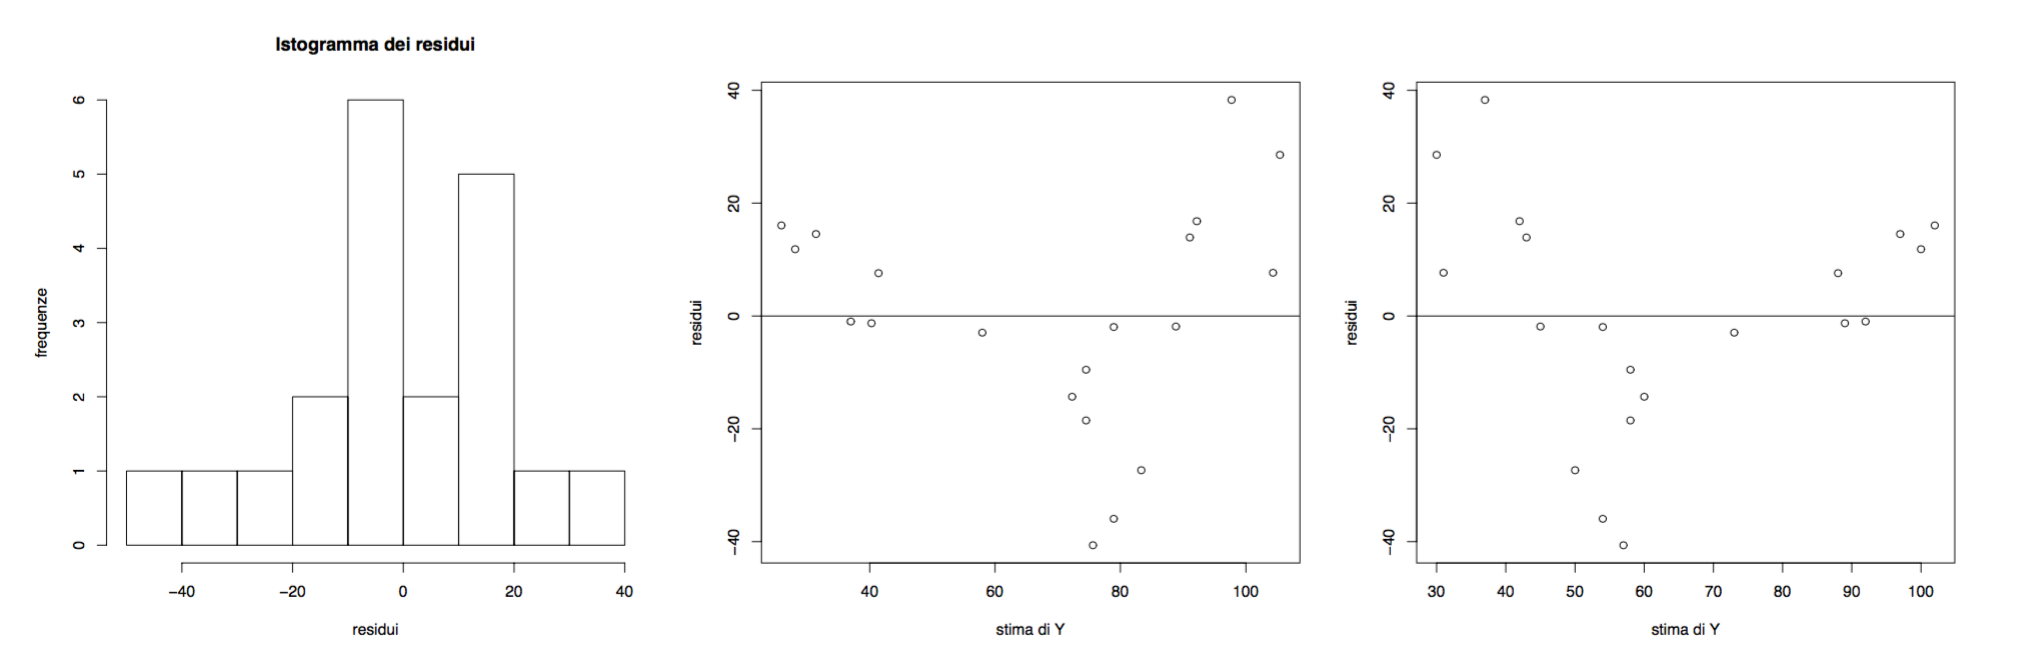
\includegraphics[width=1\textwidth]{./notes/immagini/l7-fig2.png}
	\caption{Tracciamento dei residui per il primo modello. \`{E} possibile notare la presenza di indipendente.}
\end{figure}

\section{Considerazioni sul problema e un secondo modello}\label{considerazioni-sul-problema-e-un-secondo-modello}

Considerando il problema modellato è possibile fare alcune osservazioni:

\begin{itemize}
	\item il consumatore potrebbe destinare solamente un determinato budget $ \kappa $ per l'acquisto del gas, ovvero $ x \cdot y = \kappa $.
	\item è ragionevole pensare che il consumatore debba consumare una quantità minima di gas $ \gamma $
	\item essendo il mercato del gas regolamentato, c'è un prezzo minimo di $ 7 $ centesimi al metro cubo sotto il quale non è possibile vendere il gas.
\end{itemize}

Tenendo in considerazione quanto elencato si arriva ad avere l'equazione:

$$
(x-7)(y-\gamma) = \kappa
$$

la quale può essere riscritta in un modo più simile a quella del modello lineare

$$
y = \gamma + \kappa \cdot \frac{1}{x-7}
$$

e sostituendo la variabile \textit{x} con $ z = \frac{1}{x-7} $, si ottiene proprio la stessa equazione la quale permette di calcolare la retta ai minimi quadrati.

Questo è possibile perché quello che finora è stato chiamato modello lineare è un caso particolare dei \textbf{modelli lineari nei parametri}. Ovvero la limitazione data dalla linearità non riguarda le variabili, ma riguarda solamente i \textbf{parametri} del modello.

Quando viene utilizzato il metodo dei minimi quadrati con questi modelli è necessario tenere in considerazione le trasformazioni che vengono fatte alle variabili, perché i valori calcolati ai minimi quadrati riguardano le variabili trasformate e non quelle di partenza, è necessario quindi \textbf{scalare} in modo opportuno i valori\footnote{Se viene scalata solamente la $ x $ non c'è questo problema perché i minimi quadrati considerano solamente le distanze rispetto l'asse $ y $.}.

La formulazione più generale del modello lineare è quindi

$$
g(y) = \alpha + \beta h(x) + \epsilon
$$

Il modello ottenuto per la nuova formulazione è:
\begin{verbatim}
lm(formula = gas ~ I(1/(prezzo - 7)))
Residuals:
Min    1Q  Median  3Q    Max
-29.617 -4.574 2.394 7.800 30.917
Coefficients:
Estimate Std. Error t value Pr(>|t|) 
(Intercept) 3.918 8.376 0.468 0.646
I(1/(prezzo - 7)) 3034.938 357.037 8.500 1.02e-07 *** 
---
Signif. codes: 0 ‘***’ 0.001 ‘**’ 0.01 ‘*’ 0.05 ‘.’ 0.1 ‘ ’ 1
Residual standard error: 15.19 on 18 degrees of freedom 
Multiple R-Squared: 0.8006, Adjusted R-squared: 0.7895 
F-statistic: 72.26 on 1 and 18 DF, p-value: 1.022e-07
\end{verbatim}

ovvero la retta

$$
y = 3.918 + 3034.938 \cdot \frac{1}{x-7}
$$

\begin{figure}[htbp]
	\centering
	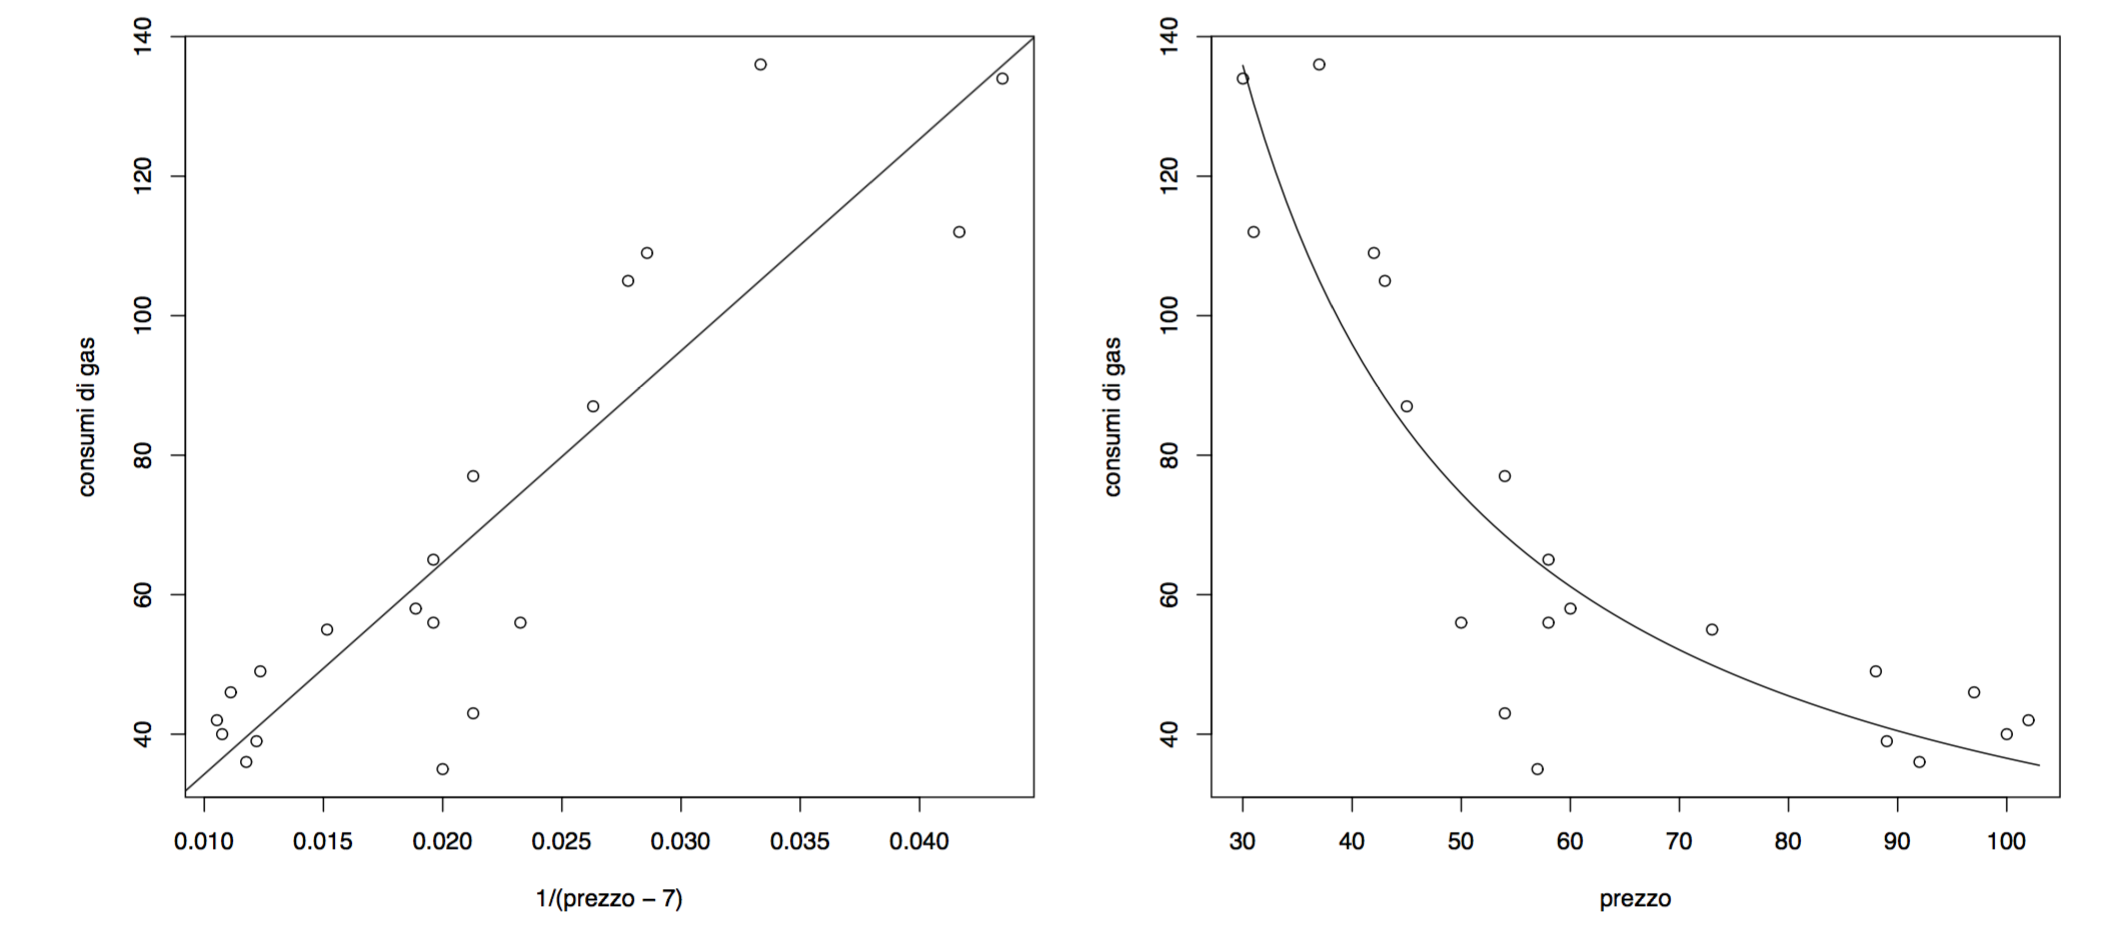
\includegraphics[width=1.1\textwidth]{./notes/immagini/l7-fig3.png}
	\caption{A destra la retta rispetto $ z $. A sinistra il modello lineare tracciato rispetto $ x $.}
\end{figure}

Dai dati del nuovo modello è possibile osservare che la varianza residua (\texttt{Residual standard error} elevato al quadrato) è passata da circa 391 a circa 207, ovvero il quadrato degli errori di previsione è stato ridotto di quasi il $ 50\% $.
Lo stesso effetto può essere visto utilizzando $ R^2 $ che da 0.6241 passa a 0.8006.

\begin{figure}[htbp]
	\centering
	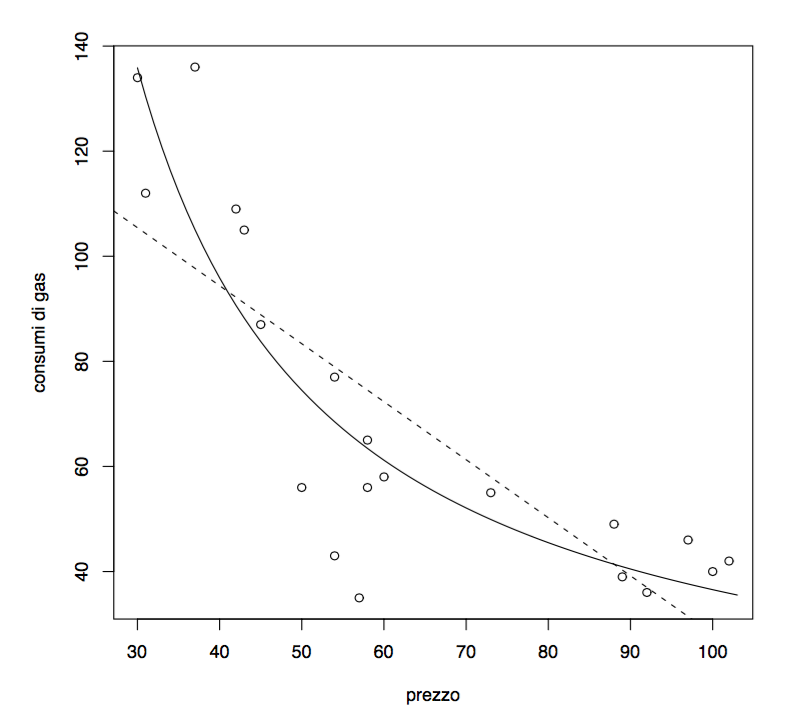
\includegraphics[width=.6\textwidth]{./notes/immagini/l7-fig4.png}
	\caption{Confronto grafico tra i due modelli.}
\end{figure}

\FloatBarrier
\section{Modello lineare con trasformate}\label{modello-lineare-con-trasformate}

\textit{Cambia il dataset di riferimento}, si vuole controllare se il reddito nazionale influisce sulla speranza di vita media dello stato. 

\begin{figure}[htbp]
	\centering
	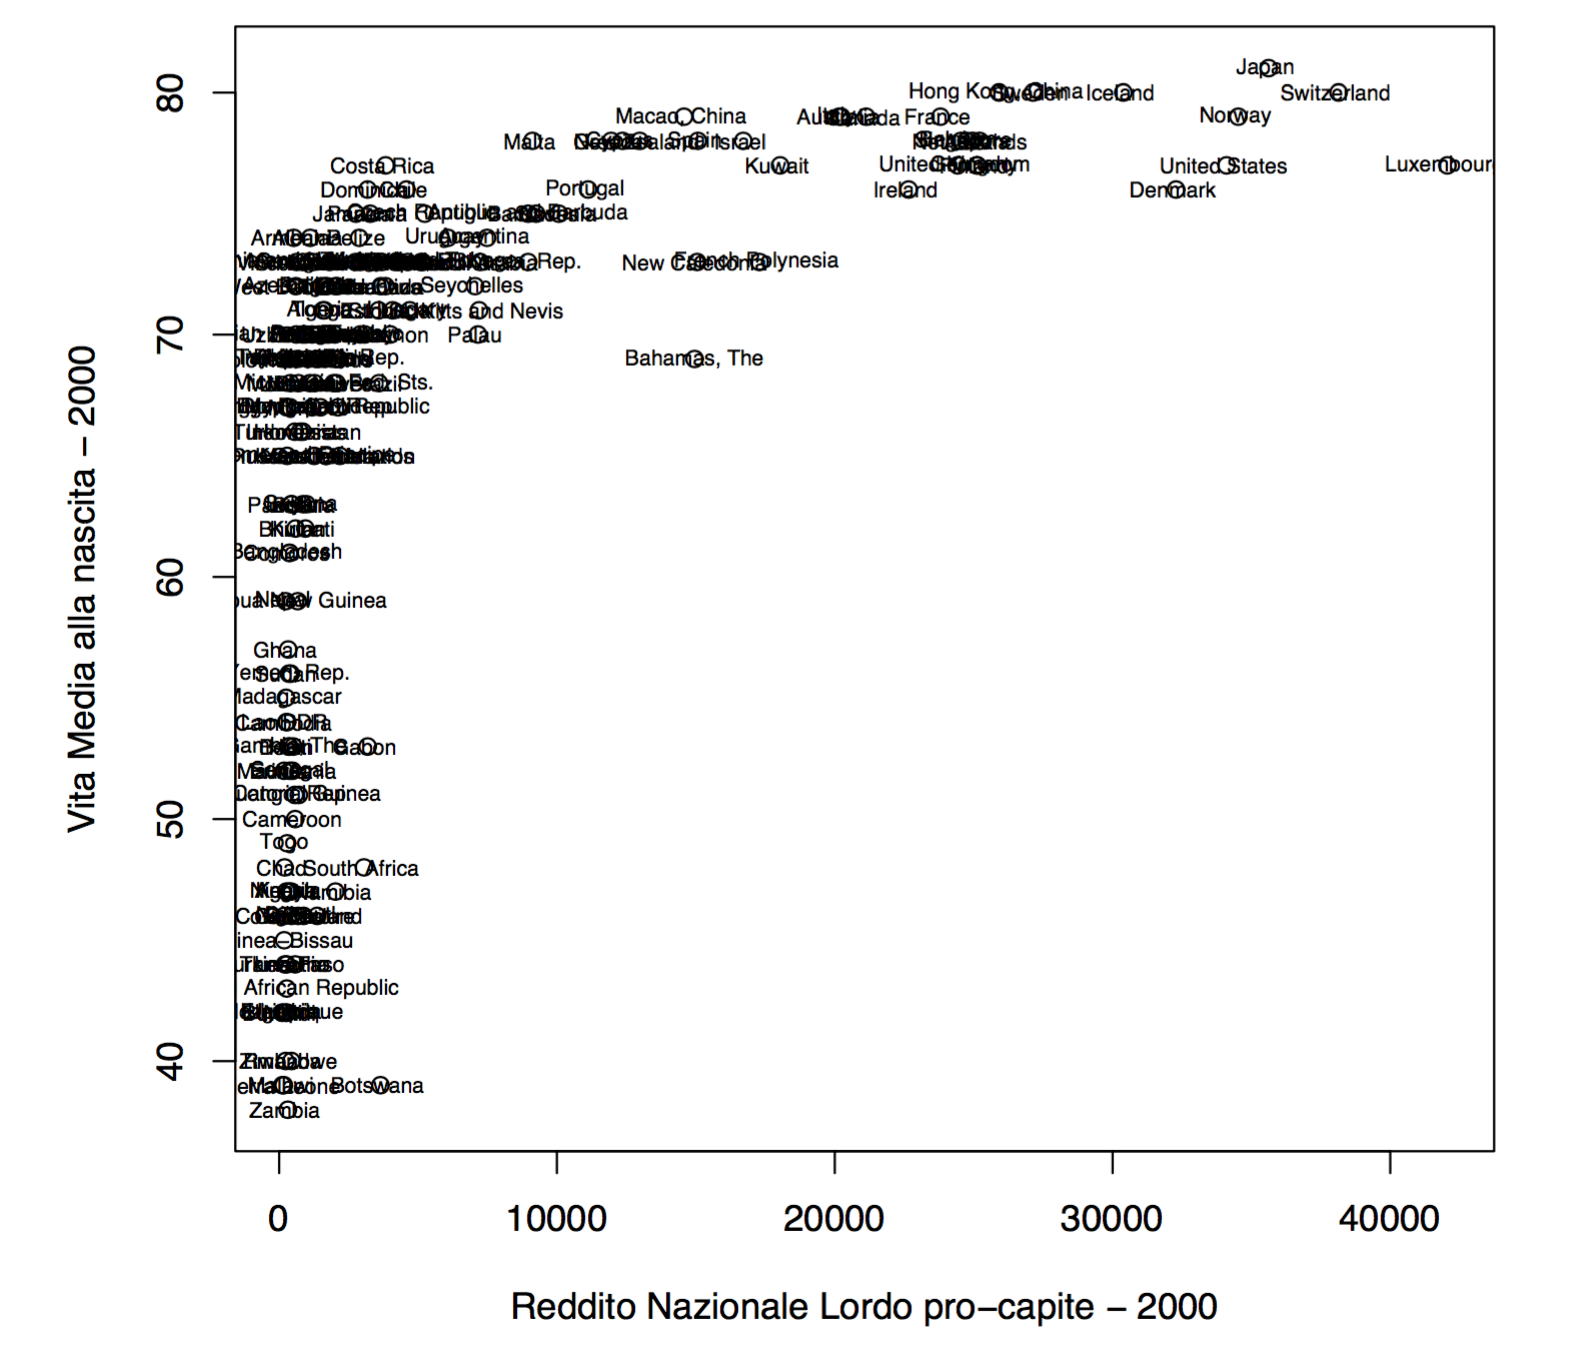
\includegraphics[width=.7\textwidth]{./notes/immagini/l7-fig5.png}
	\caption{Dataset - GNI - ELF}
\end{figure}

La prima cosa da fare è osservare come si comporta il modello lineare senza trasformazioni:

\begin{verbatim}
	lm(formula = elf ~ GNIpc)
	Residuals:
	Min    1Q  Median  3Q    Max
	-24.924 -7.512 4.119 7.431 12.948
	Coefficients:
	Estimate Std. Error t value Pr(>|t|)
	(Intercept) 6.133e+01 8.967e-01 68.390 < 2e-16 ***
	GNIpc 7.115e-04 8.230e-05 8.645 3.76e-15 ***
	---
	Signif. codes: 0 ‘***’ 0.001 ‘**’ 0.01 ‘*’ 0.05 ‘.’ 0.1 ‘ ’ 1
	Residual standard error: 9.903 on 171 degrees of freedom 
	Multiple R-Squared: 0.3041, Adjusted R-squared: 0.3 
	F-statistic: 74.73 on 1 and 171 DF, p-value: 3.757e-15
\end{verbatim}

Si può notare come l'indice $ R^2 $ sia molto basso (0.3041), ma risulta essere molto significativo perché, per il \textit{p-value} ottenuto sia ha che è improbabile che valga l'ipotesi nulla.

Tracciando il modello e il grafico dei residui è possibile notare che
\begin{itemize}
	\item La retta ottenuta non curva abbastanza e quindi non si adatta bene ai dati
	\item Il modello prevede una vita media che può essere maggiore di 90 anni, il che è abbastanza improbabile.
\end{itemize}

\begin{figure}[htbp]
	\centering
	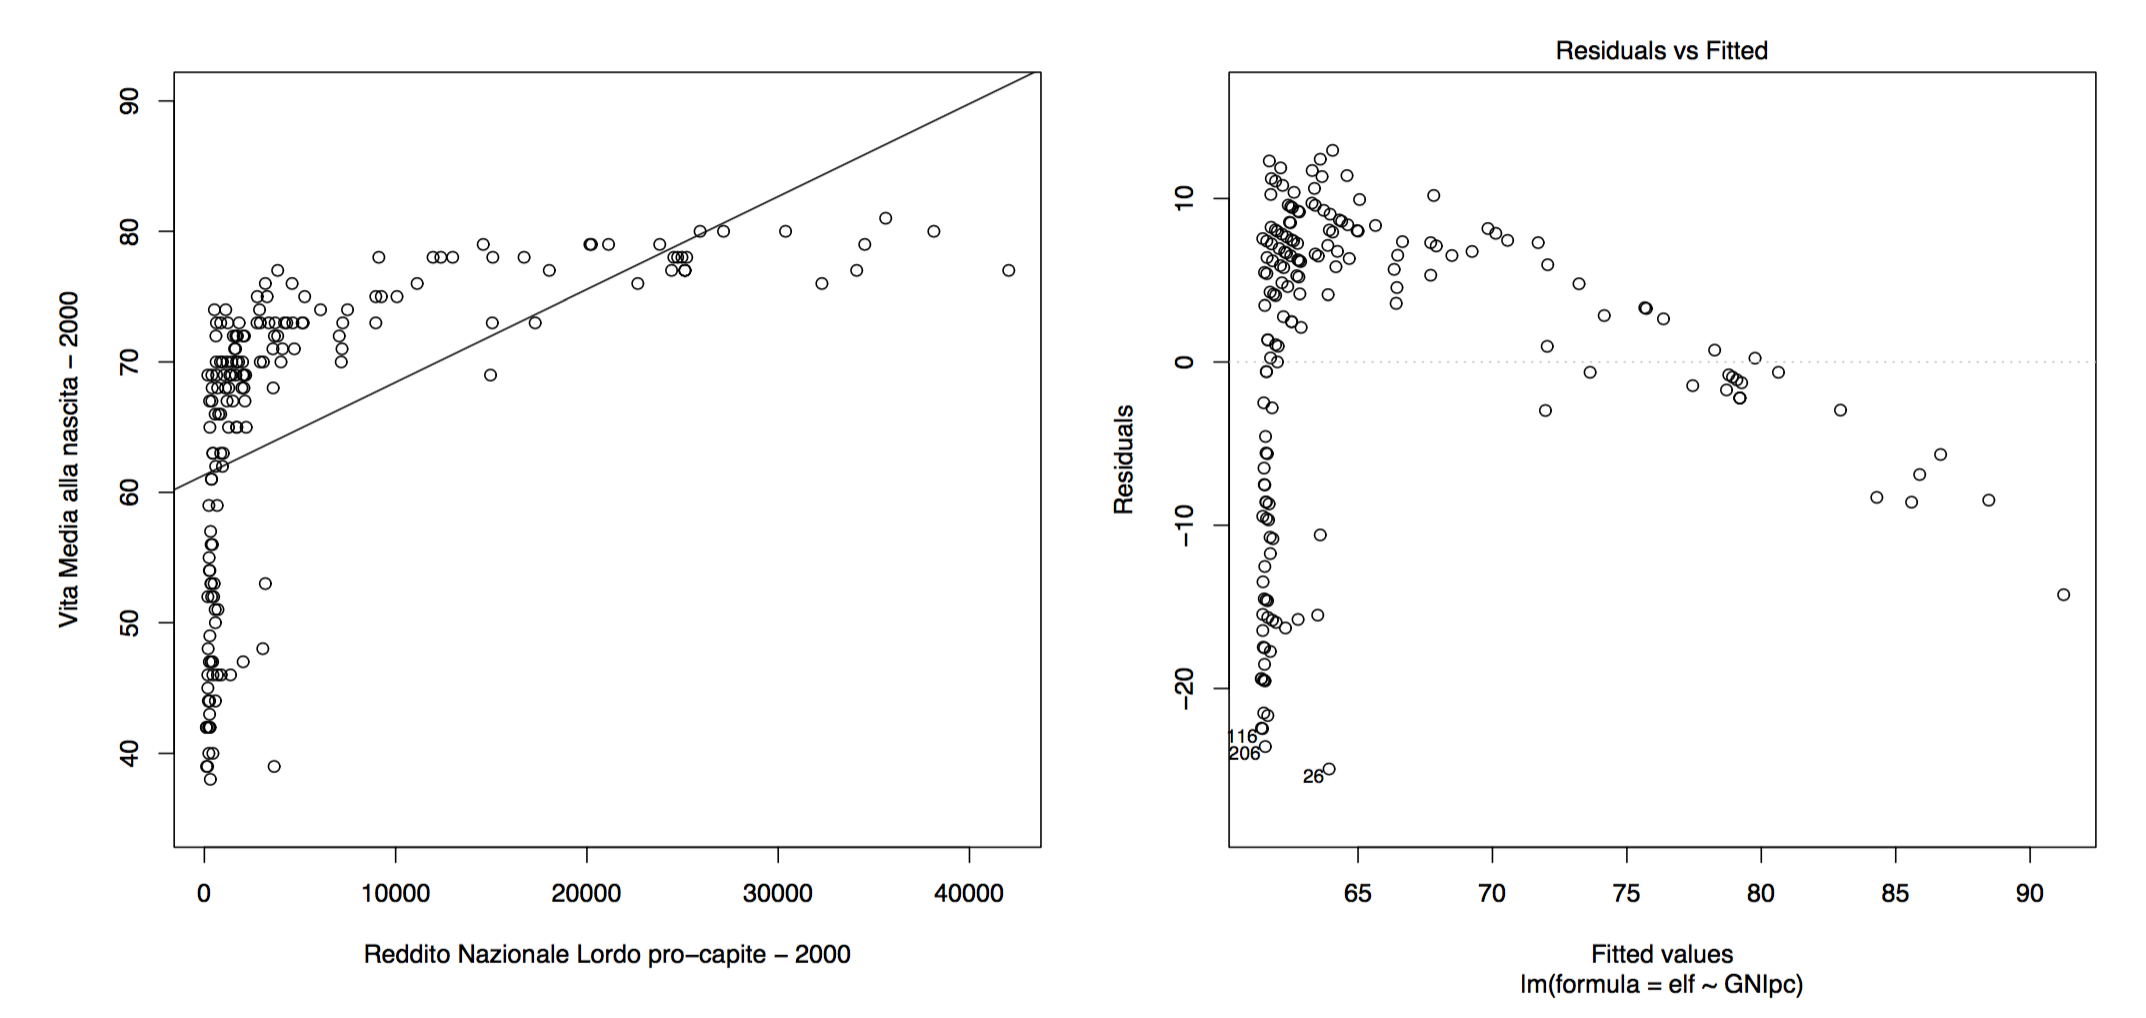
\includegraphics[width=.9\textwidth]{./notes/immagini/l7-fig6.png}
	\caption{Primo modello e residui ottenuti}
\end{figure}

Per adattare meglio la curva è possibile utilizzare la scala logaritmica per l'asse delle \textit{x}. In questo modo, al crescere del reddito viene dato via via meno peso.
Inoltre, rappresentando graficamente questa trasformazioni si ottiene una nuvola di punti più simile ad una retta.

\begin{figure}[htbp]
	\centering
	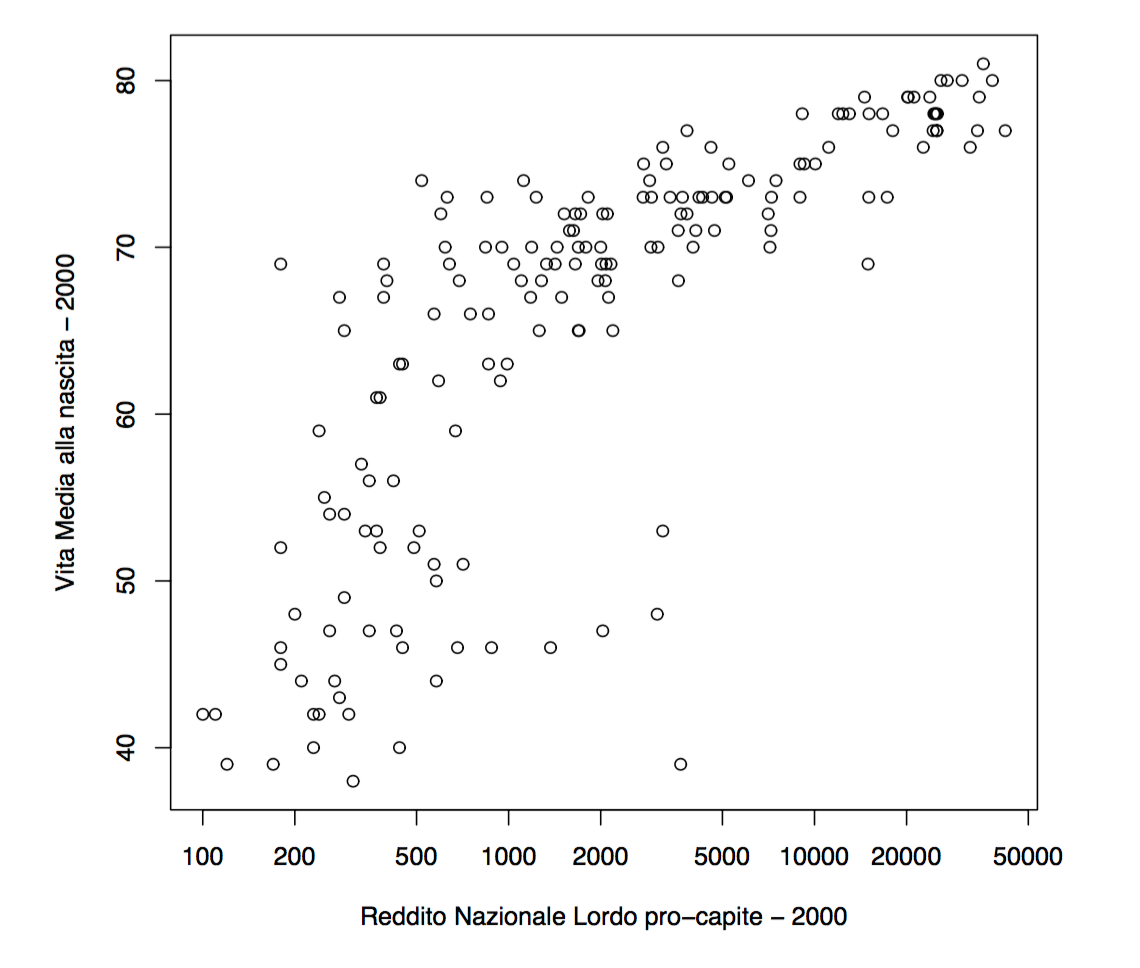
\includegraphics[width=.6\textwidth]{./notes/immagini/l7-fig7.png}
	\caption{Grafico che utilizza la scala logaritmica per i valori delle $ x $. L'asse è comunque etichettato con i valori originali.}
\end{figure}

Il modello diventa quindi

$$
(\text{vita media alla nascita}) = \alpha + \beta \log(\text{reddito nazionale pro capite})
$$

\begin{verbatim}
lm(formula = elf ~ I(logGDP), data = elf.data)
Residuals:
Min     1Q   Median   3Q     Max
-29.6591 -2.9511 0.7906 5.1050 17.4844
Coefficients:
Estimate Std. Error t value Pr(>|t|)
(Intercept) 22.6701 2.8447 7.969 2.02e-13 *** 
I(logGDP) 5.6767 0.3677 15.438 < 2e-16 ***
---
Signif. codes: 0 ‘***’ 0.001 ‘**’ 0.01 ‘*’ 0.05 ‘.’ 0.1 ‘ ’ 1
Residual standard error: 7.674 on 174 degrees of freedom 
Multiple R-Squared: 0.578, Adjusted R-squared: 0.5756 
F-statistic: 238.3 on 1 and 174 DF, p-value: < 2.2e-16
\end{verbatim}

Con questo secondo modello si ottiene un indice $ R^2 $ doppio rispetto al precedente e questo può essere osservato anche nella rappresentazione grafica del nuovo modello.

\begin{figure}[htbp]
	\centering
	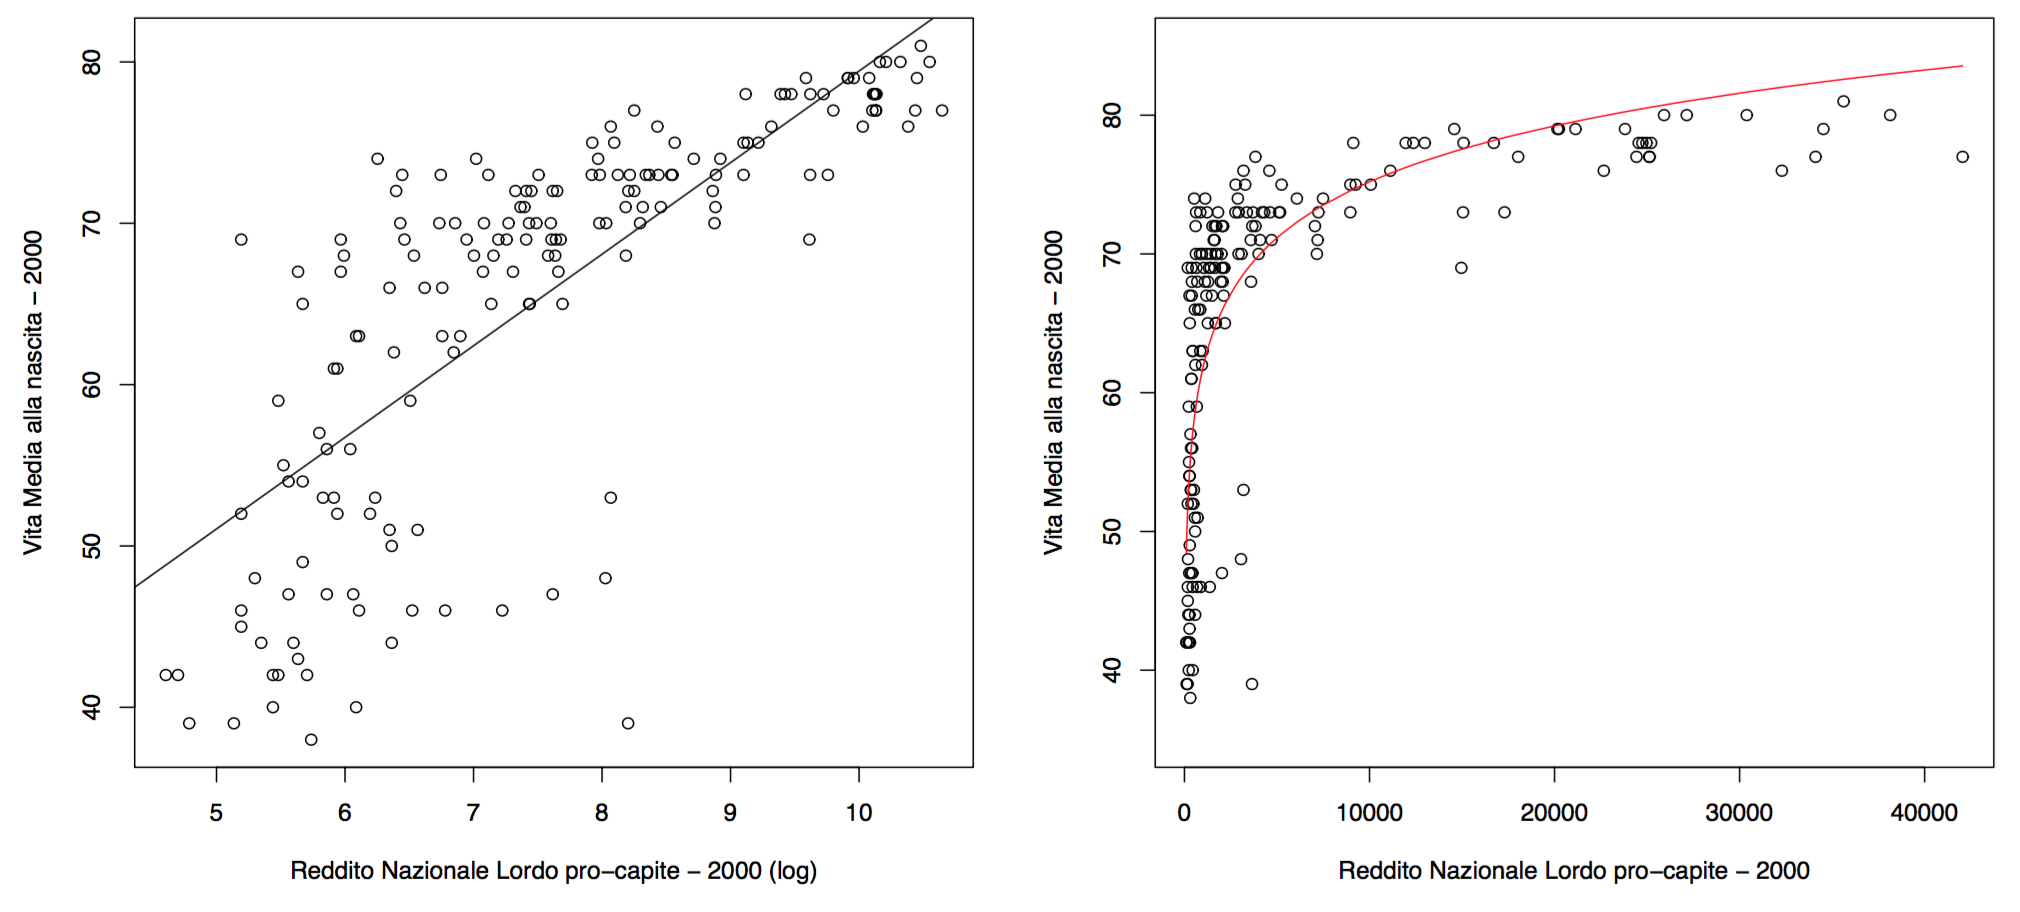
\includegraphics[width=.9\textwidth]{./notes/immagini/l7-fig8.png}
	\caption{Secondo modello: a sinistra con la scala logaritmica, a destra normale.}
\end{figure}

C'è però ancora un problema che riguarda i valori estremi che non vengono approssimati bene dalla curva e lo si può notare anche dai residui.

\begin{figure}[htbp]
	\centering
	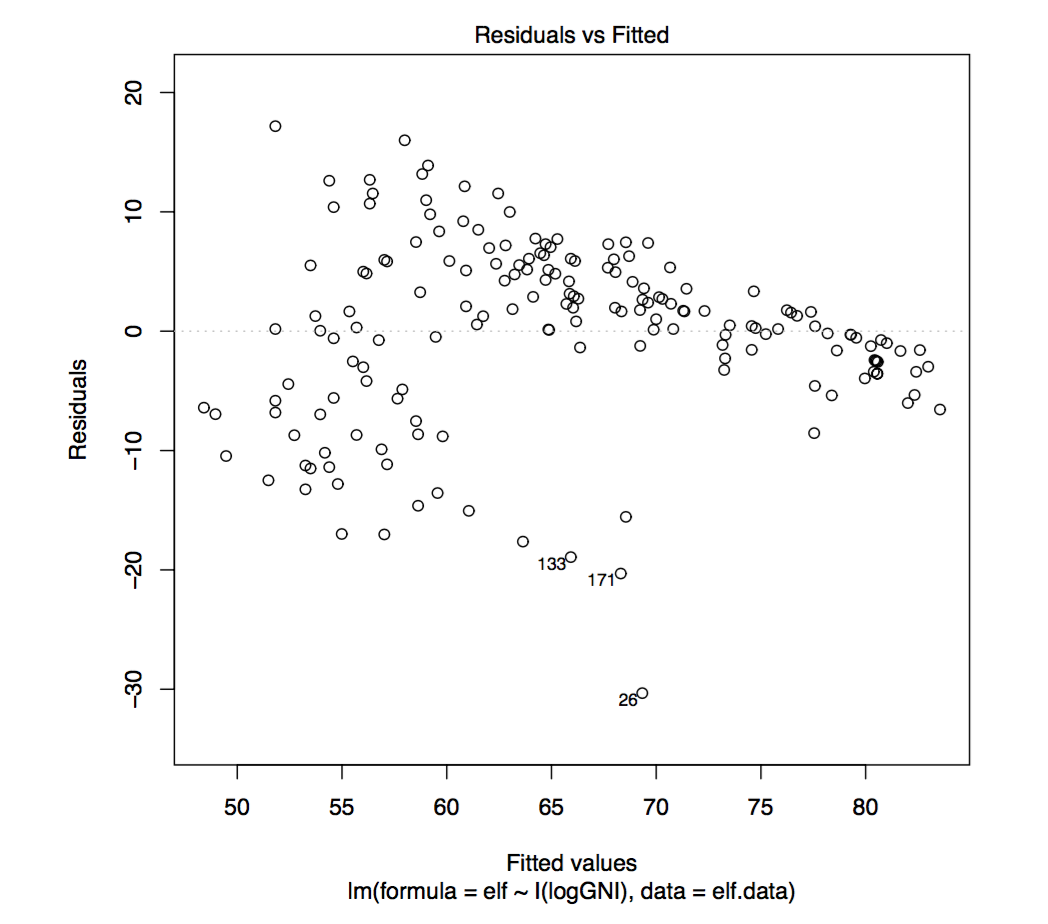
\includegraphics[width=.6\textwidth]{./notes/immagini/l7-fig9.png}
	\caption{Residui per il secondo modello }
\end{figure}

Un'ulteriore modifica può essere quella di trasformare anche la variabile risposta, elevandola alla quinta, in modo da dare maggior peso ai valori maggiori.

Il modello ottenuto è quindi dato da

$$
(\text{vita media alla nascita})^5 = \alpha + \beta \log(\text{reddito nazionale pro capite}) + \epsilon
$$

Da notare che con questa formulazione le ipotesi sugli errori (media nulla, varianza costante, distribuzione normale, ecc.) \textbf{devono valere per gli errori su scala trasformata}.

Una volta calcolato il modello si ottiene

\begin{verbatim}
lm(formula = elf.5 ~ logGNI, data = elf.data)
Residuals:
Min        1Q        Median    3Q       Max
-1.801e+09 -2.817e+08 7.965e+06 3.036e+08 1.334e+09
Coefficients:
Estimate Std. Error t value Pr(>|t|) 
(Intercept) -2.345e+09 1.832e+08 -12.80 <2e-16 *** 
logGNI 5.164e+08 2.376e+07 21.73 <2e-16 ***
---
Signif. codes: 0 ‘***’ 0.001 ‘**’ 0.01 ‘*’ 0.05 ‘.’ 0.1 ‘ ’ 1
Residual standard error: 4.89e+08 on 171 degrees of freedom 
Multiple R-Squared: 0.7341, Adjusted R-squared: 0.7326 
F-statistic: 472.2 on 1 and 171 DF, p-value: < 2.2e-16
\end{verbatim}

\begin{figure}[htbp]
	\centering
	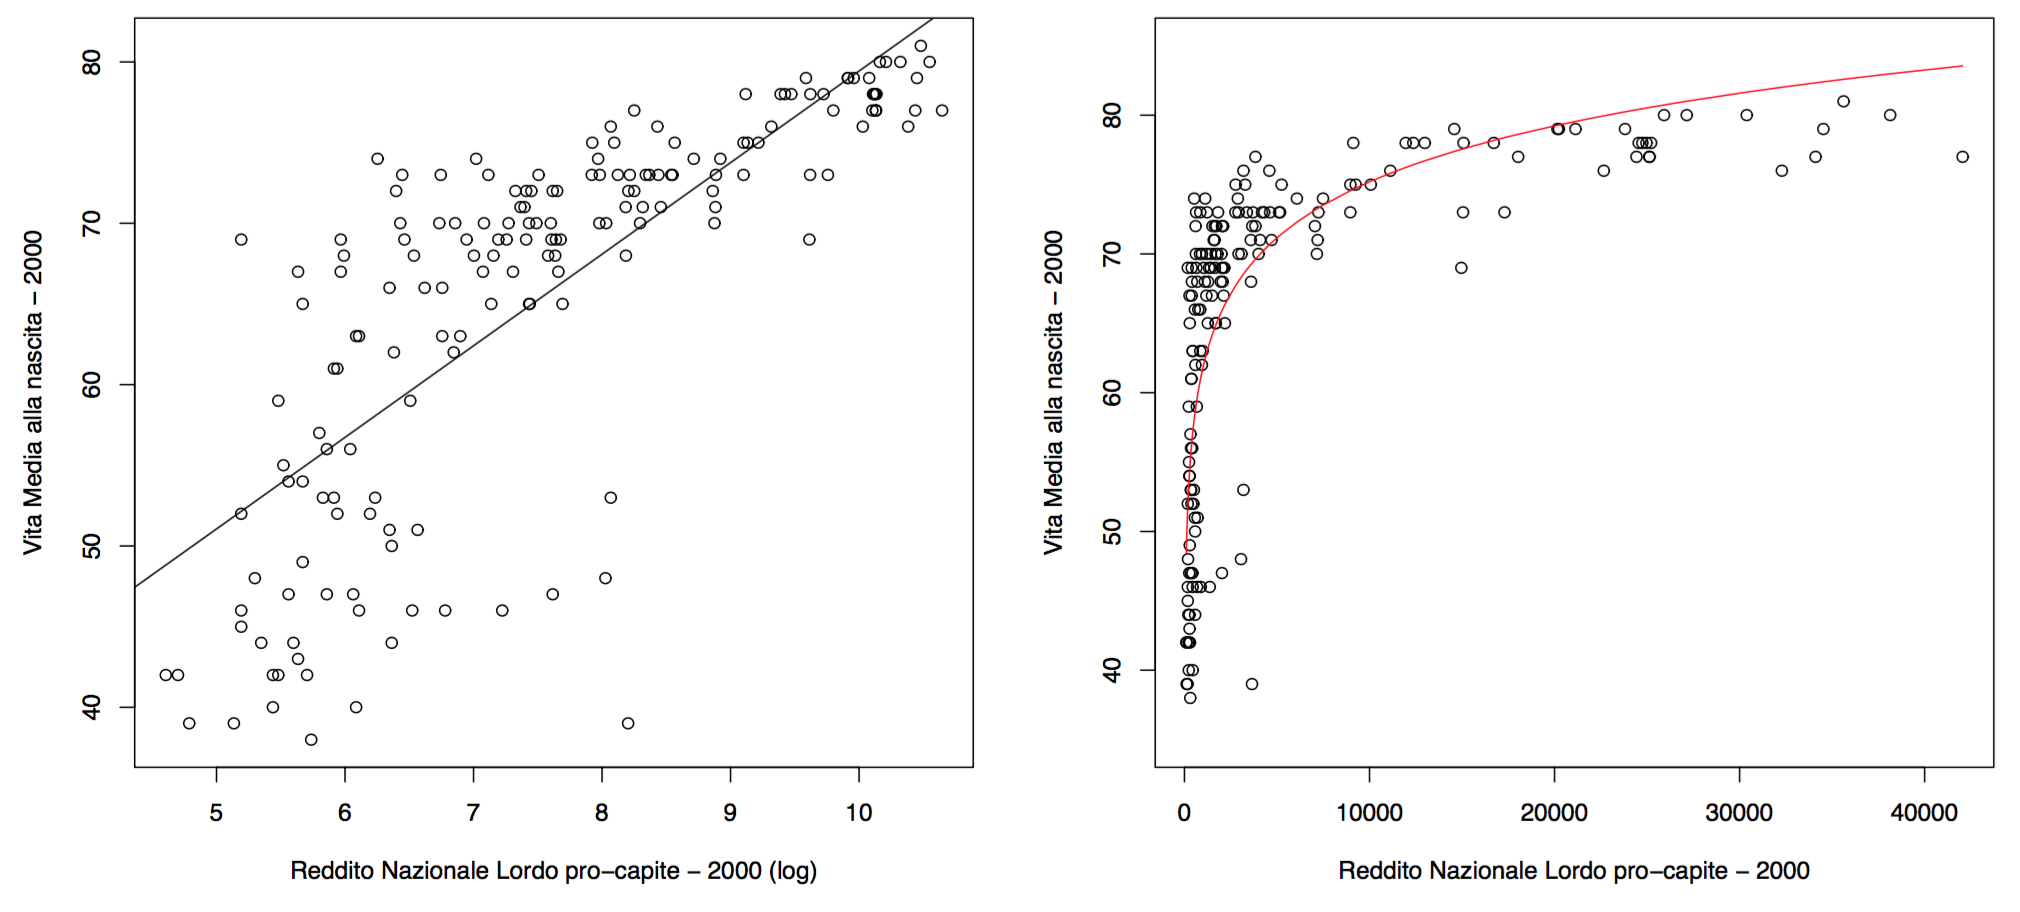
\includegraphics[width=.9\textwidth]{./notes/immagini/l7-fig8.png}
	\caption{Terzo modello: a sinistra con la scala originale e a destra i residui.}
\end{figure}

L'indice $ R^2 $ ottenuto fa riferimento ai residui calcolati sulla scala trasformata, quindi per avere un'indice di adattamento dei dati è possibile utilizzare la media dei quadrati dei residui per la variabile originale:

$$
\frac{1}{n}\sum\limits_{i=1}^n \Big[ \big(\text{vita media alla nascita}\big)_i - \big(\alpha + \beta \log(\text{reddito nazionale pro capite})_i\big)\Big]
$$

Calcolando questo valore si ottiene 55.08, mentre con il secondo modello si aveva la varianza dei residui pari a 58.89. Si ottiene quindi una riduzione del $ 6\% $ del quadrato degli errori di previsione.










\chapter{Algoritmi su stringhe}\label{algoritmi-su-stringhe}

\section{Il problema del matching esatto}\label{il-problema-del-matching-esatto}

Si ha un pattern \emph{P} di lunghezza \emph{m} e un testo \emph{T} in
cui cercare il pattern di lunghezza $n \geq m$.

Un esempio di problema è la ricerca del pattern \emph{P = aba} in
\emph{T=bbabaxababay}. In questo caso ci sono 3 occorrenze del pattern,
che si sovrappongono tra loro.

Risolvere questo problema in modo efficiente è di importanza chiave dal
momento che tutti i motori di ricerca si basano sul pattern matching
esatto o approssimato. Un altro campo in cui è utile il pattern matching
è nella bioinformatica, infatti, il DNA umano può essere visto come una
stringa di 4 miliardi di caratteri.

\subsection{Notazione utilizzata}\label{notazione-utilizzata}

Una stringa è composta da un insieme \emph{Sigma} di simboli
distinguibili e che prendono il nome di \textbf{caratteri dell'alfabeto}.

L'alfabeto, ovvero l'insieme di simboli, può essere finito oppure
infinito ed è dotato di un ordine totale tra i vari simboli.

Una successione finita dei caratteri dell'alfabeto prende il nome di
\textbf{stringa} e i caratteri che la compongono vengono indicizzati a
partire da 1.

$$
X = x_1 \ldots x_n
$$

$|X|$ indica la lunghezza di una stringa e nel
caso questa sia 0, la stringa è vuota e viene rappresentata con
$\epsilon$.

Due stringhe possono essere concatenate tra loro:

$$
X \cdot Y = x_1\ldots x_ny_1\ldots y_m
$$

e $\epsilon$ è l'elemento neutro per la concatenazione, dal momento
che la concatenazione della stringa vuota ad un'altra stringa è uguale
alla stringa di partenza.

La concatenazione multipla della stessa stringa viene indicata con
l'esponenziale:

$$
X^k = \underbrace{X \cdot \ldots \cdot X}_{k}
$$

Una \textbf{sottostringa} di una stringa \emph{X} è una stringa
\emph{Y}, tale che
$X = Z \cdot Y \cdot W$ per
qualche \emph{Z, W}.

Ogni terna \emph{(Z,Y,W)} prende il nome di \textbf{occorrenza} di
\emph{Y} in \emph{X} e si dice che la stringa \emph{Y} \textbf{occorre}
in \emph{X} nella posizione $i = |Z| + 1$.
In particolare si ha:

$$
X = Z \cdot Y \cdot W = X[1,i-1]X[i,j]X[j+1,n]
$$

Se la stringa $Z = \epsilon$, \emph{Y} prende il nome di
\textbf{prefisso}, mentre se $W=\epsilon$, \emph{Y} prende il nome
di \textbf{suffisso}.

Se la stringa \emph{Y} è sia prefisso che suffisso di \emph{X}, allora
\emph{Y} è un \textbf{bordo} della stringa \emph{X} e si ha che

$$
Y = X[1,m] = X[n-m+1,n]
$$

Prefissi, suffissi, bordi e sottostringhe vengono detti \textbf{propri}
se sono $\neq \epsilon$ e $\neq X$, altrimenti vengono detti
\textbf{degeneri}.

\subsubsection{Periodo}\label{periodo}

Se \emph{Y} è un bordo di \emph{X} allora esistono \emph{Z} e \emph{W}
tali che $X = Z \cdot Y = Y \cdot W$ con
$|Z| =|W| = p = n - m$.
\emph{p} prende il nome di \textbf{periodo} della stringa \emph{X}.

Un periodo si dice \textbf{proprio} se $0 < p <n$.

\paragraph{Lemma - Periodi e Bordi}\label{lemma---origine-del-periodo}

Il nome periodo deriva dal fatto che se $X = x_1x_2\ldots x_n$ ha
come bordo \emph{Y} di lunghezza \emph{m}. Allora $x_i = x_{i+p}$ per
ogni \emph{i} tale che $1 \leq i \leq n-p$. 
Viceversa se $x_i = x_{i+p}$, per ogni \emph{i} tale che $1 \leq i \leq n - p$ allora
$Y = X[1,n-p]$ è un bordo di \emph{X}.

\subparagraph{Dimostrazione}\label{dimostrazione}

Per definizione di bordo, \emph{Y} è un bordo di \emph{Z} se e solo se

$$
Y = X[1,m]=X[n-m+1,n]
$$

Ma $X[1,m] = X[n-m+1,n]$ se e solo se sono uguali i corrispondenti caratteri $x_i$ e $x_{i+n-m}$ per $i = 1, \ldots, m$, ma questo è come dire $x_i = x_{i+p} \forall i \: = 1,\ldots, n-p $ con $p  = n-m$. 

Pertanto, segue che la stringa \textit{X} di lunghezza \textit{n} ha un bordo \textit{Y} se e solo se \textit{p = n-m} è un periodo delle stringa.

Una stringa \emph{X} viene detta \textbf{periodica} se
$0 \leq 2p \leq n$ ovvero se c'è un bordo di lunghezza
$m  < n \leq 2m$.

\paragraph{Lemma - Concatenazione di stringhe periodiche}\label{lemma---concatenazione-di-stringhe-periodiche}

Siano \emph{X} e \emph{Y} due stringhe con periodo \emph{p} tali che $X = \alpha\gamma$ e $Y = \gamma\beta$ con $|\gamma| \geq p$.

La stringa $Z = \alpha\gamma\beta$ ha anch'essa periodo \emph{p}.

\begin{figure}[htbp]
\centering
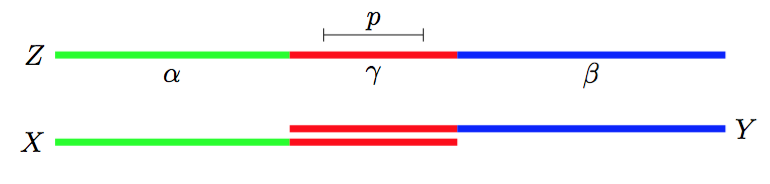
\includegraphics[width=.7\textwidth]{./notes/immagini/l10-fig1.png}
\end{figure}

\subparagraph{Dimostrazione}\label{dimostrazione-1}

Siano $ z_i $ e $ z_{i+p} $ dure caratteri di \textit{Z} a distanza \textit{p}. Siccome $ |\gamma|  \geq p$, i due caratteri possono essere appartenenti solamente o a \textit{X} o a \textit{Y} e mai ad entrambe le stringhe contemporaneamente. 
Pertanto dal momento che sia \textit{X} sia \textit{Y} hanno periodo \textit{p}, i due caratteri devono essere per forza uguali.

Da questo segue il lemma di periodicità che afferma che due periodi distinti \emph{p} e \emph{q} non possono coesistere troppo a lungo in
una stessa stringa senza che la stringa abbia anche periodo \emph{MCD(p,q)}.

\paragraph{Lemma - Lemma di periodicità}\label{lemma---lemma-di-periodicituxe0}

Sia \emph{X} una stringa di lunghezza \emph{n} con due periodi \emph{p}
e \emph{q} non entrambi nulli.

Se $n \geq p + q - MCD(p,q)$ allora la stringa \emph{X} ha anche periodo \emph{MCD(p,q)}.

\begin{figure}[htbp]
\centering
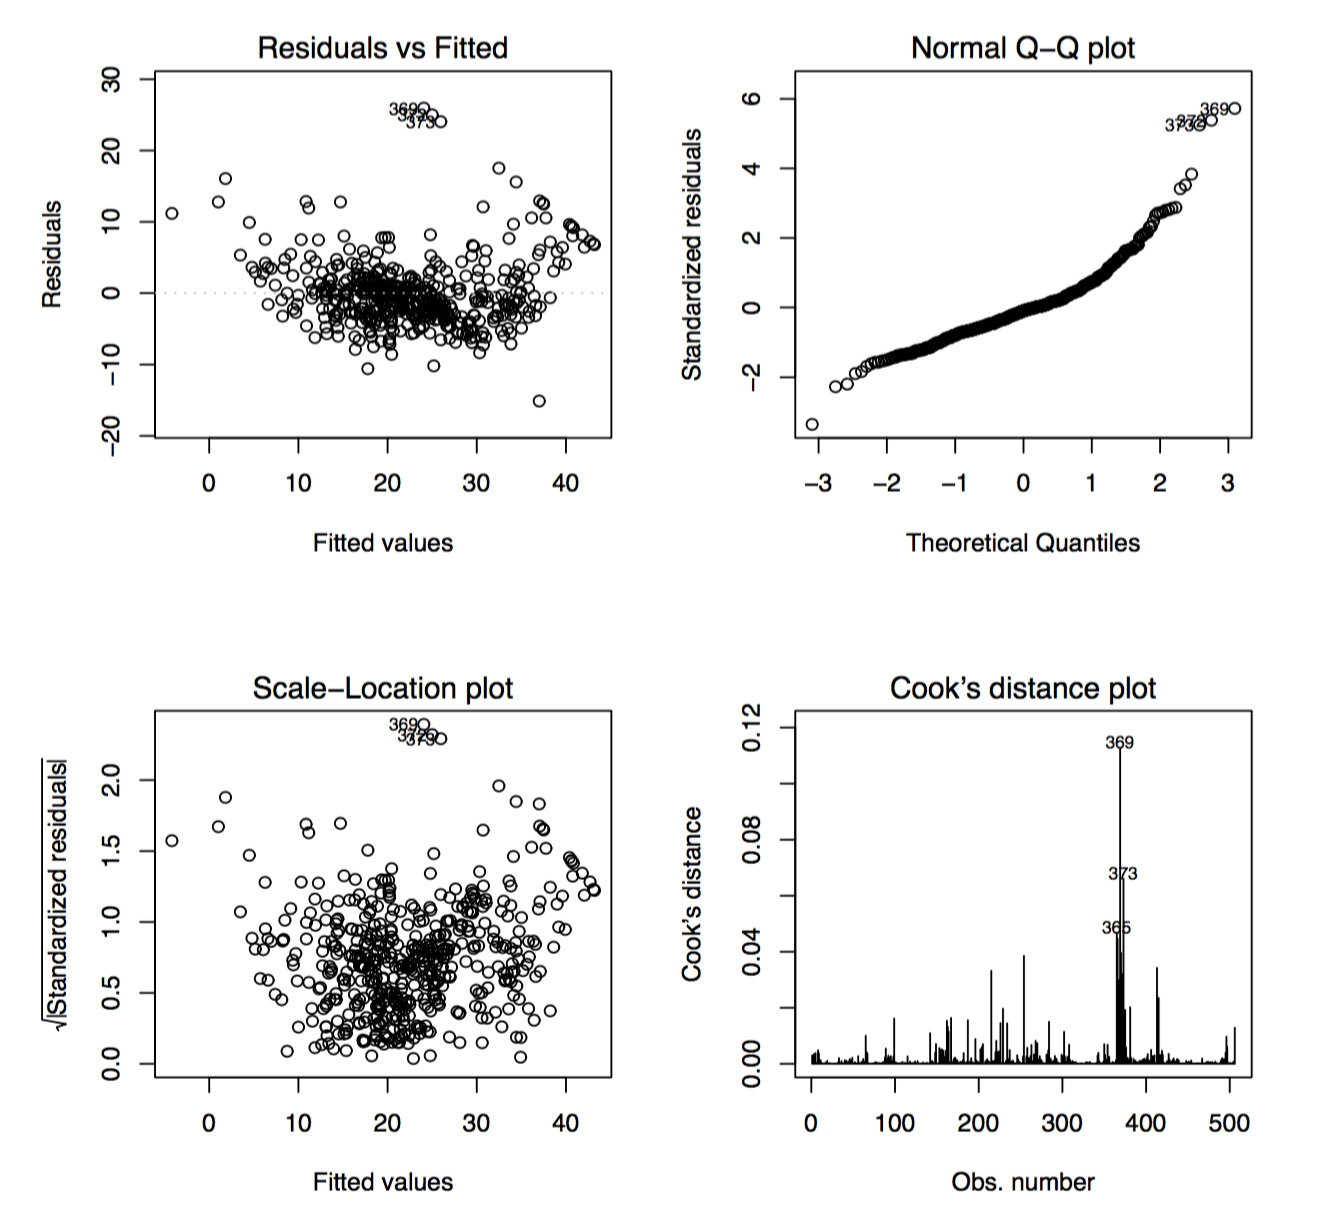
\includegraphics[width=.7\textwidth]{./notes/immagini/l10-fig2.png}
\caption{}
\end{figure}

\subparagraph{Dimostrazione}\label{dimostrazione-2}

Supponendo che $p \leq q$, la dimostrazione viene fatta per induzione su \emph{p+q}.

$(p+q = 1)$ 

Se \emph{p=0} oppure \emph{p=q=0} allora \emph{MCD(p,q) = q} e dunque
\emph{X} ha periodo \emph{MCD(p,q)} perché ha periodo \emph{q}.

$(p+q > 1)$

Se \emph{p=0} o \emph{p=q} vale ancora il caso base.

Se $1 \leq p < q$, si ha che la stringa \emph{X} ha bordi $\alpha$ e $\beta$ di lunghezza \emph{n-p} e \emph{n-q}, questo per il primo lemma dimostrato.

\begin{figure}[htbp]
\centering
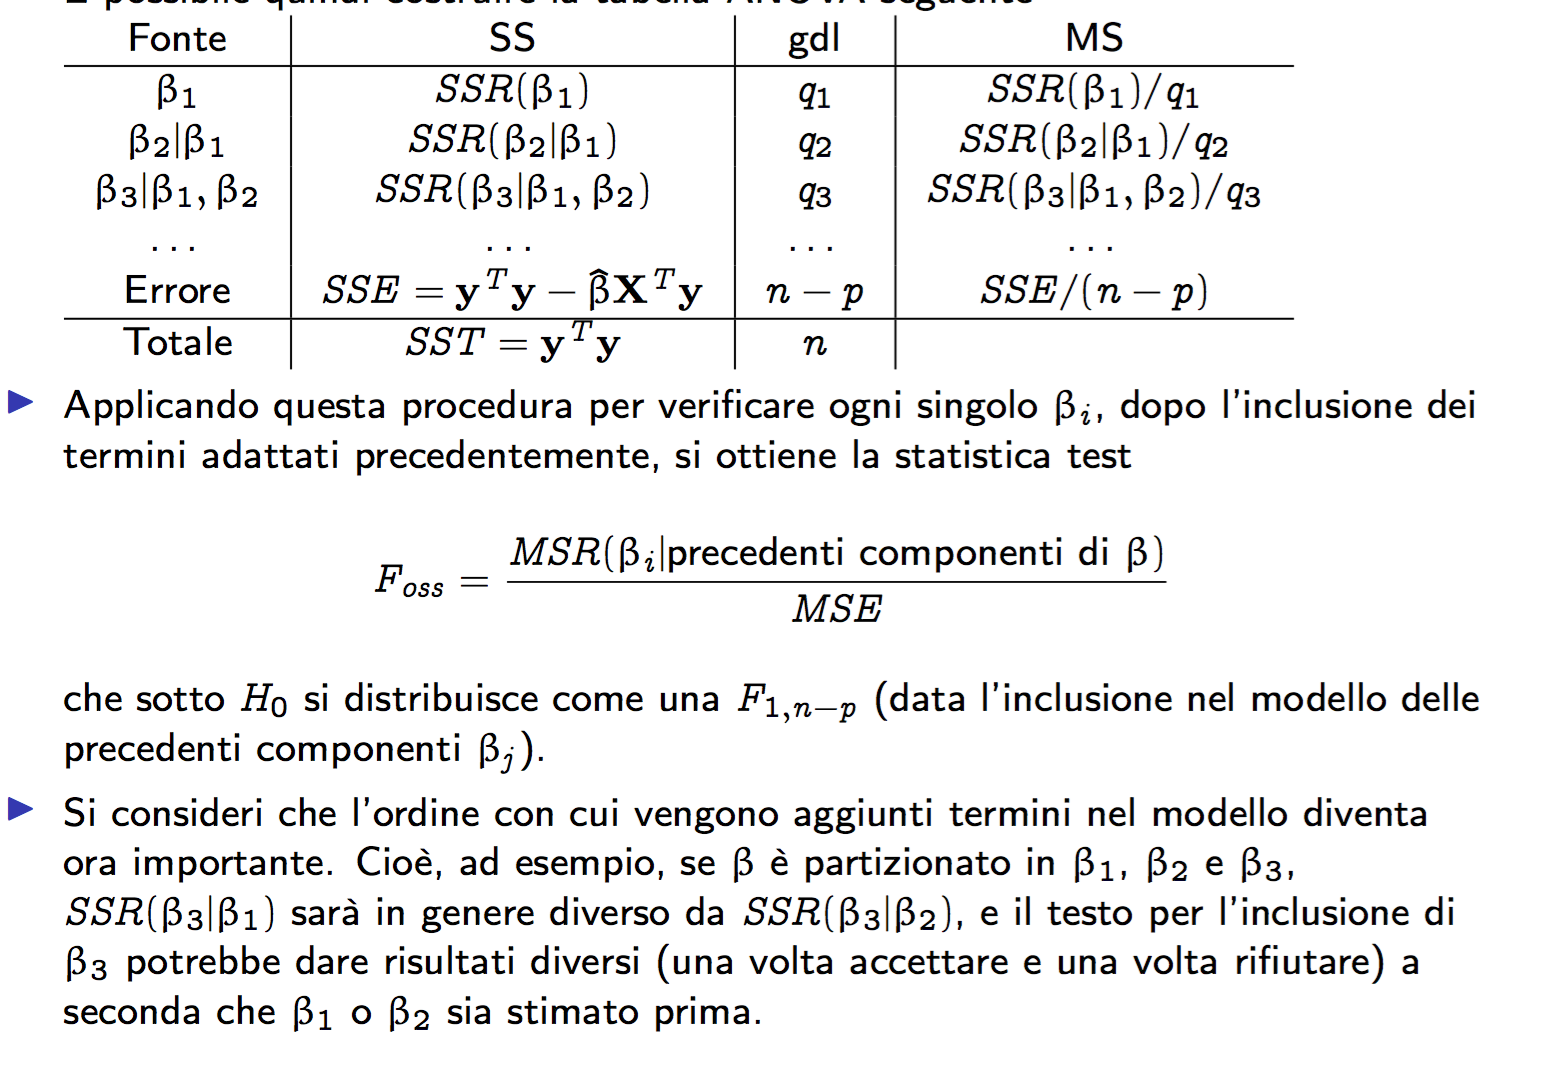
\includegraphics[width=.7\textwidth]{./notes/immagini/l10-fig3.png}
\caption{In verde la stringa $\alpha$ che si ripete con periodo
\emph{p}. In blu la stringa $\beta$ che si ripete con periodo
\emph{q}}
\end{figure}

La stringa $\beta$ essendo bordo di \emph{X} è anche bordo $\alpha$ dal momento che $\alpha$ è un bordo di \emph{X}, pertanto $\alpha$ ha periodo $r = |\alpha| - |\beta| = q -p$.

Si ha che $p+r < p + q$ e \emph{MCD(p,r) = MCD(p,q)}, quindi per ipotesi induttiva

$$
|\alpha| = n - p \geq q - MCD(p,q) = p+r+MCD(p,q)
$$

$ \alpha $ ha quindi come periodo sia \textit{r} (a causa di $ \beta $), sia \textit{p} (per ipotesi), ovvero ha periodo \textit{MCD(p,r)} che per come è definito \textit{r} è uguale a \textit{MCD(p,r)}.

Si ha quindi che

\begin{align*}
	2|\alpha| &= (n-p) + (n-p) \\
					 &\geq q - MCD(p,q) + (n-p) \\
					 &\geq n
\end{align*}

perché $ p < q $ per ipotesi e $ MCD(p,q) \leq q - p $ per le proprietà del massimo comun divisore.

Questo implica che il prefisso $ \alpha $ di \textit{X} e il suffisso $ \alpha $ di \textit{X} coprono tutto \textit{X} e pertanto le due stringhe devono sovrapporsi\footnote{Non è possibile applicare il lemma della concatenazione perché non si sa di quanto queste stringhe si sovrappongono.} oppure $ X = \alpha\alpha $.

Presi quindi due caratteri $ x_i $ e $ x_j $ della stringa \textit{X}, tali che $ j - i = MCD(p,q) $ può succedere che i due caratteri appartengano alla stessa $ \alpha $ e quindi siano uguali, perché $ \alpha $ ha periodo $ r = MCD(p,q) $ oppure che $x_i \in \alpha_{(prefisso)} \text{ e } x_j \in \alpha_{(suffisso)} $.

\begin{figure}[htbp]
	\centering
	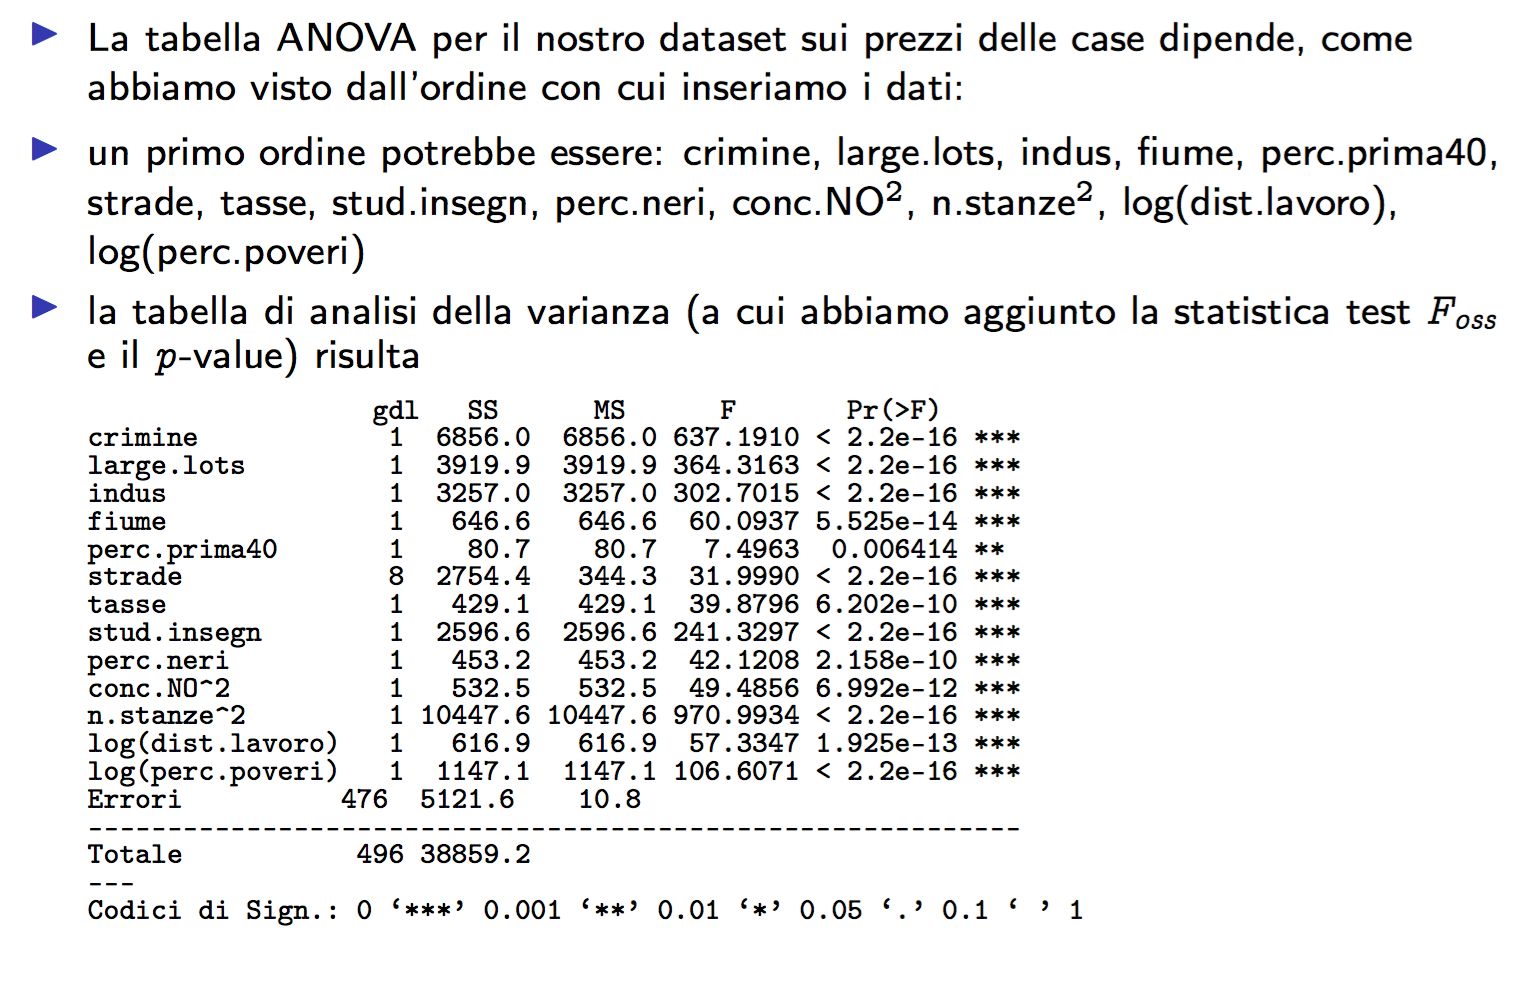
\includegraphics[width=.7\textwidth]{./notes/immagini/l10-fig4.png}
\end{figure}


In questo caso si ha che $ j > n - |\alpha| = p $ e quindi $ j - p \geq 1$. Si può quindi considerare il carattere $ x_{j-p} = x_j$ per via del periodo \textit{p} di $ \alpha $ e che risulta appartenere a $ \alpha_{(prefisso)} $ perché $ p \geq MCD(p,q) $.

La distanza tra $ x_{j-p} \text{ e } x_i$ è \textit{p - MCD(p,q)}, che per definizione è un multiplo di \textit{MCD(p,q)}, pertanto si ha che $ x_{j-p} \text{ e } x_i$ appartengono ad $ \alpha_{(prefisso)} $ che ha periodo \textit{MCD(p,q)}, pertanto $ x_{j-p} = x_i = x_j $ e di conseguenza \textit{X} ha periodo \textit{MCD(p,q)}.


\section{Lezione 11 - Pipeline di apprendimento supervisionato}\label{lezione-11---pipeline-di-apprendimento-supervisionato}

L'apprendimento supervisionato può essere visto come una serie di fasi:

\begin{enumerate}
\item
  Analisi del problema
\item
  Raccolta, analisi e preprocessing dei dati
\item
  Studio delle correlazioni tra variabili
\item
  Feature selection, definizione dei pesi, normalizzazione
\item
  Scelta del predittore e del modello
\item
  Verifica del modello
\end{enumerate}

\subsection{Fase 4 - Feature selection, definizione dei pesi, normalizzazione}\label{fase-4---feature-selection-definizione-dei-pesi-normalizzazione}

Per rappresentare gli oggetti con i quali lavora un algoritmo di apprendimento è possibile utilizzare varie rappresentazioni:

\begin{itemize}
\item
  \textbf{vettori} contenti valori reali, ad esempio un vettore che descrive lo stato di salute di un paziente con il valore di pressione del sangue, il battito cardiaco, altezza e peso.
\item
  \textbf{stringhe}: una serie di caratteri che rappresentano un documento o la struttura del DNA
\item
  \textbf{insiemi}: ad esempio l'insieme di termini che compare in un documento
\item
  \textbf{array multidimensionali}: come immagini e video
\item
  \textbf{albero o grafi}: un documento XML
\item
  \textbf{strutture composte}: ottenute combinando tra loro le
  precedenti.
\end{itemize}

Nel corso ci concentriamo principalmente sui vettori.

Per ogni oggetto possiamo avere a disposizione delle \textbf{feature categoriche}, che rappresentano delle caratteristiche nominali
dell'oggetto (marca di un auto, paese di origine), alcune di queste
possono essere anche \textbf{ordinali}, cioè che impongono un ordine tra
gli elementi ma la distanza tra un valore e un altro non è
quantificabile, come per esempio i gradi militari: soldato, caporale,
ecc.

Un altro tipo di feature sono le \textbf{feature quantitative}, cioè
delle caratteristiche che sono \textbf{enumerabili}, come il livello di
apprezzamento di un prodotto, oppure \textbf{ratio}, ovvero dei numeri
reali, come il peso di una persona.

\subsubsection{Mapping Feature categoriche}\label{mapping-feature-categoriche}

Per gestire le feature categoriche, queste vengono mappate in un vettore con tante
componenti quanti sono i possibili valori della variabile (\textbf{one-hot}).

Ad esempio per rappresentare la marca, il colore e la tipologia di una macchina è possibile codificare le tre feature con:

\begin{itemize}
\item
  Marca: Fiat {[}c1{]}, Toyota {[}c2{]}, Ford {[}c3{]}
\item
  Colore: Bianco {[}c4{]}, Nero {[}c5{]}, Rosso {[}c6{]},
\item
  Tipo: Economica {[}c7{]}, Sportiva {[}c8{]}
\end{itemize}

La macchina\textit{ (Toyota, Rossa, Economica)} viene rappresentata con un
vettore $ [ \underbrace{0,1,0,}_{\text{marca}} \underbrace{0,0,1,}_{\text{colore}} \underbrace{1,0,}_{\text{tipo}}]$.


\subsubsection{Mapping per feature continue}\label{mapping-per-feature-continue}

Tipicamente le feature continue vengono trasformate per ottenere dei valori comparabili con le altre feature.

Per ottenere ciò è possibile applicare una delle seguenti trasformazioni:

\begin{itemize}
\item
  \textbf{Centramento}: $f(x) = x - E(x)$
\item
  \textbf{Normalizzazione STD}: $f(x) = (x - E(x))/\sigma(x)$
\item
  \textbf{Rescaling}: $f(x) = (x - x_{min})/(x_{max}-x_{min})$
\end{itemize}

Dove:

\begin{itemize}
\item
  \emph{E(x)} è la media di tutti i possibili valori di \emph{x}
\item
  $\sigma (x)$ è lo scarto quadratico medio
\end{itemize}

\subsection{Algoritmo K-NN}\label{algoritmo-k-nn}

\textbf{K-Nearest-Neighbors} è un algoritmo di classificazione in cui 
un esempio di test è classificato come la classe di maggioranza dei sui
\emph{k}-vicini nel training set.

Si vanno a scegliere i \emph{k} elementi più vicini all'elemento che si
vuole classificare e viene scelta come classe quella della maggioranza
dei suoi \emph{k}-vicini.

Trattandosi di vettori la distanza tra i vari esempi viene misurata con

$$ || x - y ||^2 = ||x||^2 + ||y||^2 - 2x^Ty$$


Per semplificare i calcoli, si può tenere in considerazione che se i due
vettori hanno la stessa norma, la loro distanza è uguale alla
similarità indotta dal prodotto scalare:

$$ || x - y ||^2 = const - 2x^Ty $$

Inoltre, è possibile normalizzare i valori dentro i vettori per ridurre il rumore.

Resta da stabilire quale valore utilizzare per \textit{k} e questo viene tipicamente fatto nella fase di \textbf{Model Selection}. 

\subsection{Fase 5 - Scelta del predittore e del modell}\label{fase-5---scelta-del-predittore-e-del-modell}

I parametri di un algoritmo di apprendimento sono i valori che influiscono nell'apprendimento, come i
vari pesi \emph{w} delle reti neurali. 

Gli \textbf{iper-parametri} sono tutti gli
altri parametri che non influiscono con l'apprendimento, come il numero
di unità nascoste per le reti neurali o il \emph{k} per l'algoritmo
k-NN.

La fase in cui questi valori vengono scelti prende il nome di
\textbf{model selection} e come valori si cerca di scegliere il migliore
per il task.

\subsubsection{Bias e varianza}\label{bias-e-varianza}

Per valutare le predizioni di uno stimatore vengono utilizzate due
misure:

\begin{itemize}
\item \textbf{bias}: che misura la distorsione di una stima quando lo stimatore è corretto: $b = E[\hat{\theta}] - \theta$ dove $\theta$ è il valore corretto e $\hat{\theta}$ è la stima del valore effettuata dal predittore.

\item \textbf{varianza}: che misura la dispersione delle stima: $v = E[(\hat{\theta} - E[\hat{\theta}])^2 ]$
\end{itemize}


\subsubsection{Hold out}\label{hold-out}

Una strategia per ricercare il valore ottimo per un iper-parametro è
quella dell'\textbf{hold out}, ovvero per ogni possibile valore un
valore per l'iper-parametro si fa eseguire l'apprendimento allo
stimatore su un sotto-insieme del training set, dopodiché si confrontano
i risultati ottenuti effettuando delle predizioni su un insieme di
validazione, ovviamente viene scelto il valore dell'iper-parametro che
porta ad ottenere le predizioni migliori.

Più formalmente:

\begin{enumerate}
\def\labelenumi{\arabic{enumi}.}
\tightlist
\item
  Si sceglie un piccolo sottoinsieme \emph{Tr} del training set che
  viene utilizzato come set di validazione \emph{Va}.
\item
  Il classificatore (algoritmo) apprende utilizzando gli esempi in
  \emph{Tr} ma senza usare quelli che compaiono in \emph{Va}.
\item
  Si osserva come si comporta il classificatore con un determinato
  valore dell'iper-parametro, e si ripete a partire dal punto 2 per
  tutti i possibili valori dell'iper-parametro.
\end{enumerate}

In questo modo riesco a calcolare l'\emph{accuracy} per ogni valore del
iper-parametro e di conseguenza posso scegliere il valore migliore.

Con l'\textbf{accuracy} si intende la proporzione di predizioni corrette
effettuate dallo stimatore.

Una volta scelto il valore, tipicamente si ri-effettua l'apprendimento
utilizzando il training set completo.

\subsubsection{K-fold Cross Validation}\label{k-fold-cross-validation}

Alternativa all'hold-out che permette di valutare in modo più preciso la
bontà dei possibili valori per un iper-parametro.

L'insieme di apprendimento viene partizionato in \emph{k} parti
disgiunte. Viene poi eseguito l'apprendimento utilizzando \emph{k-1}
partizioni e utilizzando la restante partizione per fare validazione.
L'intero processo di apprendimento viene ripetuto quindi \emph{k} volte,
utilizzando ogni volta una diversa partizione per la validazione.

Così facendo per un singolo valore di un iper-parametro si ottengono
\emph{k} valori di accuracy e si può utilizzare la media di questi valori
per ottenere una stima dell'accuracy migliore.

Il tutto viene poi ripetuto per ogni possibile valore
dell'iper-parametro.

Il valore di \emph{k} influisce sulla dimensione del training set:
utilizzando un \emph{k} piccolo si ottiene un training set più piccolo,
quindi il bias induttivo aumenta e la varianza della stima ottenuta
diminuisce.

Viceversa, se \emph{k} è grande, il training set è più grande e si
ottiene un minor bias induttivo.

Tipicamente si usa \emph{k=5} o \emph{k=10}.

Se \textit{k=|Tr|} questo approccio prende il nome di \textbf{leave-one-out}.

\subsubsection{Valutazione per dati non bilanciati}\label{sec:pre-rec}

Quando nel training set c'è una classe che domina sulle altre,
l'accuracy non è più una stima adatta, vengono quindi utilizzate altre
misure quali: \textbf{precision}, \textbf{recall} e \textbf{F-Measure}.

Infatti, se c'è una classe di maggioranza, l'accuracy di un predittore che classifica tutti gli esempi
con la classe di maggioranza può risultare più elevata di quella di un predittore che effettua delle predizioni
utilizzando altri criteri.

\begin{itemize}
\item
  \textbf{Precision}: ($\pi$) misura quante volte, quanti tra gli esempi
  classificati come positivi sono effettivamente positivi, ovvero il grado di correttezza del sistema
  $$ \pi = \frac{true \: positive}{true \: positive + false \: positive}$$  

\item   \textbf{Recall}: ($\rho$) misura quanti che sono effettivamente positivi
  sono stati classificati come positivi, ovvero il grado di completezza del sistema
  
  $$ \rho = \frac{true \: positive}{true \: positive + false \: negative}$$  
 \item  \textbf{F-measure}: combina precision e recall:
  \begin{align*}
	F_{\beta} &= \frac{(1+\beta)^2\pi\rho}{\beta^2\pi + \rho} \\
	F_1 &= 2\frac{\pi\rho}{\pi + \rho}
  \end{align*} 
\end{itemize}
 
% !TEX encoding = UTF-8
% !TEX program = pdflatex
% !TEX root = MEMOC.tex
% !TEX spellcheck = it-IT

\section{Recap sul branch and bound}

Termino quando non ci sono più nodi. In questo caso la soluzioni ottima è quella incumbent. Tipicamente però non si raggiunge la terminazione dell'algoritmo per questioni di tempo o memoria.

Se mi fermo prima della terminazione ho la garanzia che incumbent è almeno una soluzione feasible. Sappiamo inoltre che, dato che i valori rilassati sono numeri reali, la soluzione ottima per il problema intero è compresa tra il valore della soluzione incumbent e il più grande upper-bound.
Si può quindi definire un intervallo di ottimalità e fermarsi quando questo gap è inferiore di una certa soglia.
Anche se il gap è molto piccolo, non vuol dire che si è vicini alla soluzione ottima, infatti il branch and bound fa fatica a chiudere i gap piccoli.

Si parte quindi dal problema iniziale $P_0$ che è il problema originale senza i vincoli di integrità, lo si risolve e poi si aggiunge un nuovo vincolo del tipo $x_i \leq k_i$. Si ripete quindi questo procedimento fino a quando non si raggiunge la condizione di stop.

Ovviamente non conviene far ripartire da capo la risoluzione del problema lineare rilassato, ma è meglio utilizzare una strategia simile alla column-generation.
Tuttavia non possiamo far ripartire il simplesso dalla soluzione corrente $\overline{x}_{LR}$  (il pedice $LR$ sta per linear relaxation), perché il nuovo vincolo che è stato aggiunto è stato scelto appositamente per rendere infeasible la soluzione corrente.
Tuttavia, la soluzione del problema duale $\overline{u}$ rimane ottima e anche per il nuovo problema duale. Si può quindi utilizzare un metodo del \textit{dual-simplex} per ottenere una soluzione ottima per il nuovo problema primale in poche iterazioni.

(Nelle dispense c'è una grande parte che a noi non interessa)


\section{Polyheadral approch to LP}

\`E un altro modo per risolvere un problema di programmazione lineare intera (o mista).

Come riferimento utilizziamo il classico problema di minimizzazione in forma standard, con un sotto-insieme di variabili $x_i$ tali che $x_i \in \mathbb{Z}\: \forall i \in I$.

L'insieme dei vincoli e delle condizioni di integralità definiscono la feasibile-region del problema, una griglia di punti interi che sono racchiusi in un poliedro definito dal sistema $Ax = b, x \geq 0$.

Ma il poliedro $Ax=b, x \geq 0$ non è l'unico. Questo può essere visto a livello grafico: la nuova di punti della feasibile-region può essere racchiusa anche da un poliedro diverso da $Ax = b, x\geq 0$, che può essere genericamente definito come $A'x = b', x\geq0$.

Ricapitolando:
\begin{itemize}
	\item La feasible region è l'insieme dei punti feasibile per il problema LP.
	\item Una forumulation è un qualsiasi poliedro che racchiude tutti e soli i punti della feasible region. Per una stessa feasibile region è possibile trovare un numero infinito di formulation.
\end{itemize}  

Quindi in MILP ogni problema ha un numero infinito di possibili formulazioni e queste possono essere viste come i rilassamenti del branch and bound.
Pertanto sarebbe conveniente scegliere come rilassamento un poliedro che è il più possibile vicino alla soluzione intera ottima, perché poliedri (formulation) più piccoli danno bound migliori.
C'è da tenere conto che non sempre è possibile determinare se una formulation è più grande o più piccola dell'altra, perché può succedere che nessuna delle due contenga esattamente l'altra.

Più formalmente, la formulazione $\{Ax = b, x\geq0\}$ è \textbf{migliore} di un'altra formulazione $\{A'x = b', x\geq0\}$ per lo stesso problema quando:

$$
\underbrace{\{Ax = b, x\geq0\}}_{polyhedron} \subseteq \{A'x = b', x\geq0\}
$$

ovvero i punti di un poliedro sono tutti contenuti all'interno dell'altro poliedro. Ovviamente questo può essere determinato in modo algebrico.

Come problema d'esempio prendiamo \textbf{Uncapacitated Facility Location} (\textbf{UFL}): ci sono $n$ location $i = 1, \ldots, n$ dove possiamo costruire delle facilities. Ci sono $m$ utenti da soddisfare con le facilities $j = 1 \ldots m$. Ogni utente deve essere soddisfatto da solamente una facility. Servire un utente ha un costo $c_{ij}$. C'è anche un costo fisso $f_i$ da pagare se viene aperta una facility in location $i$.

La formulazione del problema è

\begin{itemize}
	\item $y_i = \begin{cases}
	1\quad&\text{apro una facility in }i \\
	0\quad&\text{altrimenti }i \\
	\end{cases}$
	\item $x_{ij} = \begin{cases}
	1\quad&\text{se la facility \textit{i} serve l'utente \textit{j}}\\
	0\quad&\text{altrimenti}
	\end{cases}$
	\item FO: $$
		\min \sum \limits_{i=1}^{n} f_i y_i + \sum\limits_{i,j} c_{ij}x_{i,j}
	$$
	\item ST: 
	\begin{itemize}
		\item $ \sum\limits_{i} x_{ij} = 1 \quad \forall j = 1 \ldots m$
		\item $x_{ij} \leq y_i \: \forall \: i,j$ oppure $\sum\limits_{j} x_{i,j} \leq M y_i  \:\forall i $
		\item $ 0 \leq x_{ij} \leq 1$, $ 0 \leq y_i \leq 1 \forall i,j$ 
		\item $ x_{ij}, y_i \in \mathbb{Z} $
	\end{itemize}
\end{itemize}

Le due formulazioni sono equivalenti, ma la prima richiede un maggior numero di vincoli. Come valore di $M$ per la seconda formulazione possiamo utilizzare il numero di utenti $m$, perché il massimo valore della sommatoria è $m$ ed avere un $M$ minimo porta ad avere dei buoni vincoli.

Ma quale delle due soluzioni conviene scegliere? Tipicamente meno vincoli ci sono, più è facile da risolvere il problema, ma avere tanti vincoli può portare ad avere un poliedro più piccolo.

Si può verificare che la prima formulazione è migliore, nel senso che definisce un poliedro più piccolo, perché se $(\overline{x},\overline{y})$ soddisfa la prima formulazione, questa soddisfa anche la seconda formulazione. 

Perché la coppia soddisfa tutti i vincoli del tipo
$$
\overline{x}_{ij} \forall\:i\forall\:j (*)
$$
e, fissato un $i$, la sommatoria di tutti quei vincoli su $j$ diventa:

$$
\sum\limits_{j} \overline{x}_{ij} \leq m \overline{y}_i
$$

ovvero $(\overline{x},\overline{y})$ soddisfa anche il vincolo della seconda formulazione.
Si può anche dimostrare che il contrario non vale.

Rimane comunque il dubbio su quale sia conveniente implementare, perché quando la formulazione geometricamente migliore è quella con più vincoli, c'è il rischio che il risolutore faccia comunque più fatica a trovarla. L'unica cosa che si può fare è provare.

A livello geometrico è comunque possibile definire la \textbf{formulazione ideale}, ovvero quella che è geometricamente migliore.
La soluzione ideale è quindi il \textbf{convex hull} della feasibile region, ovvero il minimo \textbf{convex set} che contenente la feasbile-region.
Un convex set $C$ è un insieme di punti, tali che $\forall x,y \in C$, il segmento che li congiunge è completamente contenuto in $C$.
Tutti i poliedri associati ad una formulation sono sempre dei convex set. 

Il \textbf{Fundamental theorem of Integer Linear Programming} dice che dato un (M)ILP (sotto forma di massimo), tale che la matrice $A$ contenga solo valori razionali\footnote{un calcolatore non riesce ad implementare i numeri razionali.}, il convex hull della feasible region è un poliedro, ovvero può essere espresso come $\{Cx\leq d, x\geq0 \}$. Non dimostriamo questo teorema.

Quindi dato un (M)ILP di massimo che definisce una feasbile region $X$, per questo teorema $convex(X)$ è un poliedro, ovvero $convex(X) = \{Cx\leq d, x \geq 0 \}$ che è anche la formulazione ideale.

La formulazione ideale gode di una \textbf{proprietà fondamentale}: se massimizzo o minimizzo $c^Tx$ utilizzando la formulazione ideale ($convex(X)$) ottengo sempre una soluzione ottima intera anche se risolvo il rilassamento continuo con il simplesso. Ovvero posso utilizzare variabili continue al posto di quelle intere, semplificando così il problema, e ottenere comunque una soluzione intera.

Serve quindi un modo per ottenere $convex(X)$, che non è cosa semplice (NP-Complete).














% !TEX encoding = UTF-8
% !TEX program = pdflatex
% !TEX root = MEMOC.tex
% !TEX spellcheck = it-IT

% 15 Dicembre 2016

\todo[inline]{Da recuperare}
% !TEX encoding = UTF-8
% !TEX program = pdflatex
% !TEX root = InformationRetrieval.tex
% !TEX spellcheck = it-IT

% 18 Novembre 2016
%\chapter{Valutazione dei sistemi di reperimento}
%\section Il paradigma Cranfield

MANCA LA PRIMA PARTE

\section{Recall}

Il richiamo misura quanti documenti rilevanti sono stati recuperati, rispetto la totalità dei documenti rilevanti presenti all'interno del pool. Anche in questo caso si tratta di un valore compreso tra 0 e 1, dove 1 indica la run perfetta.

\begin{figure}[htbp]
	\centering
	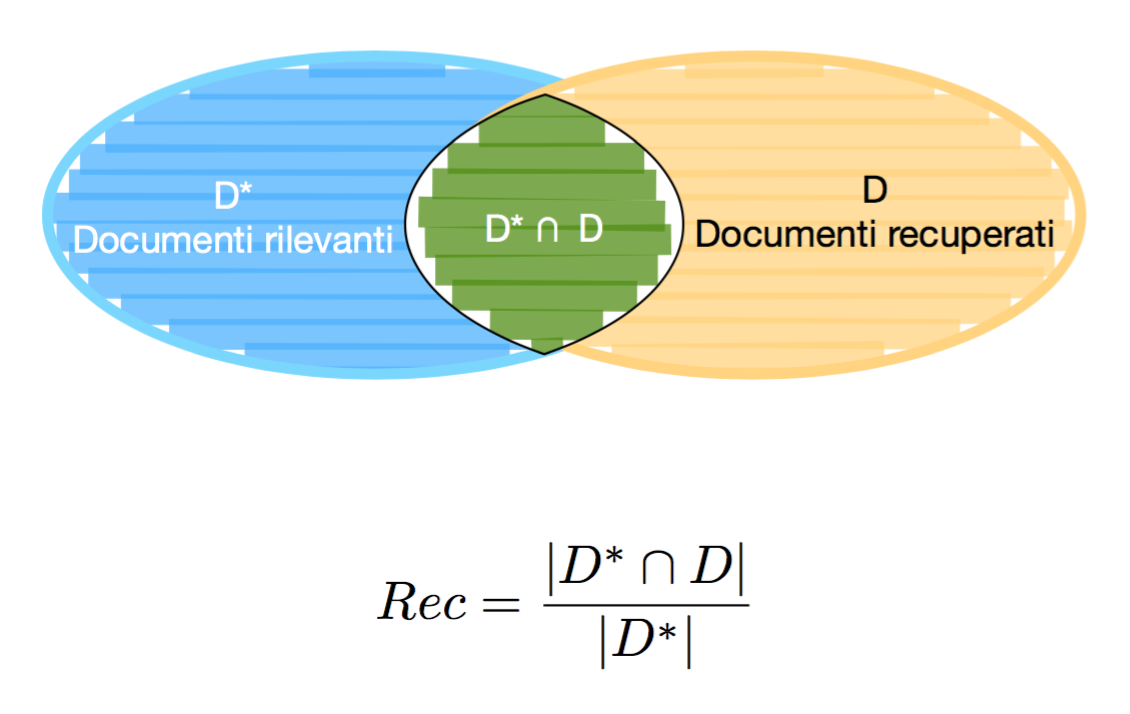
\includegraphics[width=0.6\textwidth]{images/l15-fig-1.png}
\end{figure}

Il valore $|D^*|$ è anche chiamato \textbf{recall base} per un determinato topic e come già detto è valore fisso che dipende dal numero di documenti rilevanti presenti nel pool o ground truth.

Più formalmente, sia $D$ un insieme finito di documenti, $T$ un insieme finito di topic, $GT$ la ground truth defin ita su $D$ e $T$ e rel un insieme totalmente ordinato di giudizi di rilevanza. La \textbf{recall base} è definita come:

\begin{align*}
	RB : T &\to \mathbb{N} \\
		t &\to RB_t = \Big| \big\{ d \in D | GT(t,d) \succ \min(REL) \big\} \Big|
\end{align*}

\begin{figure}[htbp]
	\centering
	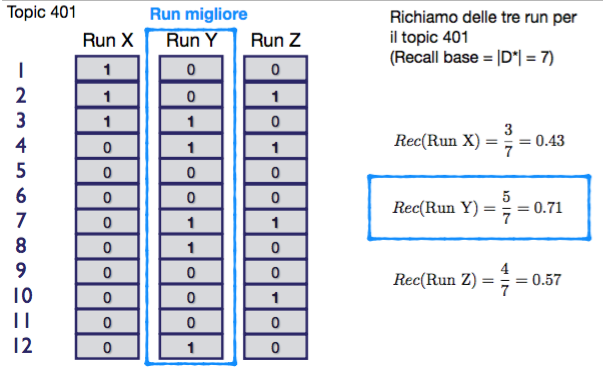
\includegraphics[width=0.7\textwidth]{images/l15-fig-2.png}
	\caption{Esempio di calcolo della recall.}
\end{figure}

\section{E-Measure e F-measure}

\`E utile avere un numero unico per esprimere la qualità della run e che riesca a combinare la precisione e il richiamo

\begin{figure}[htbp]
	\centering
	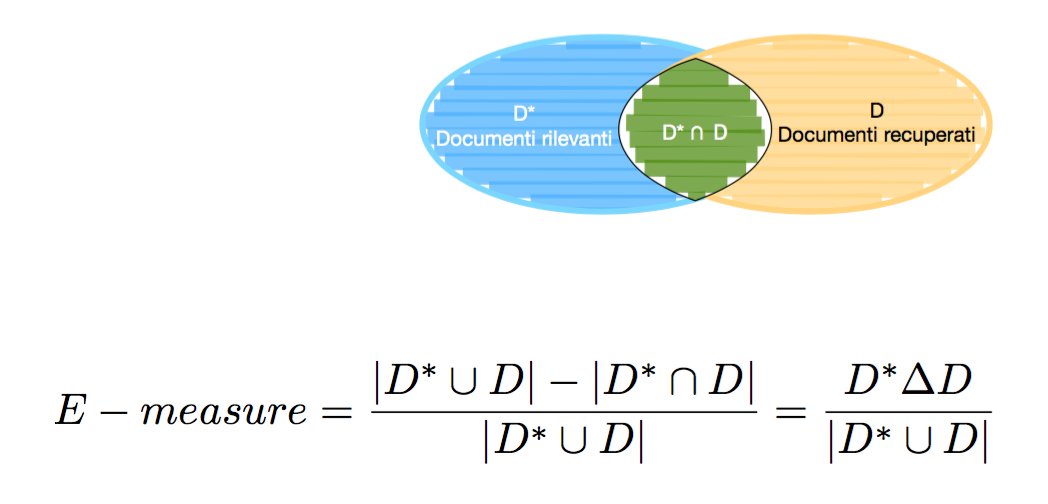
\includegraphics[width=0.7\textwidth]{images/l15-fig-3.png}
\end{figure}

Se l'intersezione è vuota, ottengo un e-measure è 1, che è il caso di retrieval pessimo.
Se invece l'e-meausre è 1, i due insiemi coincidono e quindi il retrieval è perfetto.

Siccome questa misura è contro-intuitiva si è scelto di utilizzare

$$
F-measure = 1 - E\text{-}measure
$$

Tuttavia, anche questa misura, come precision e recall, non è una misura ranked, perché non viene preso in considerazione l'ordine.


\section{Precisione con cut-off}

Per alcuni task di ricerca è importante tenere in considerazione l'ordine dei risultati e quindi è utile avere delle misure che tengano conto anche di questo.

L'idea quindi è quella di calcolare la precisione solamente sui primi $k$ elementi recuperati. Questa nuova misura prende il nome di $perc@k$.

Un caso particolare è quello di $p[RB_t]$ che è la precision con cut-off dato dalla dimensione della recall base per un dato topic.

\section{Curva Richiamo-Precisione}

Questa curva calcola la precisione in funzione di $x$ punti di richiamo, in modo da poter disegnare una curva con i punti di richiamo sull'asse delle ascisse e la precisione sulle ordinate.

\begin{figure}[htbp]
	\centering
	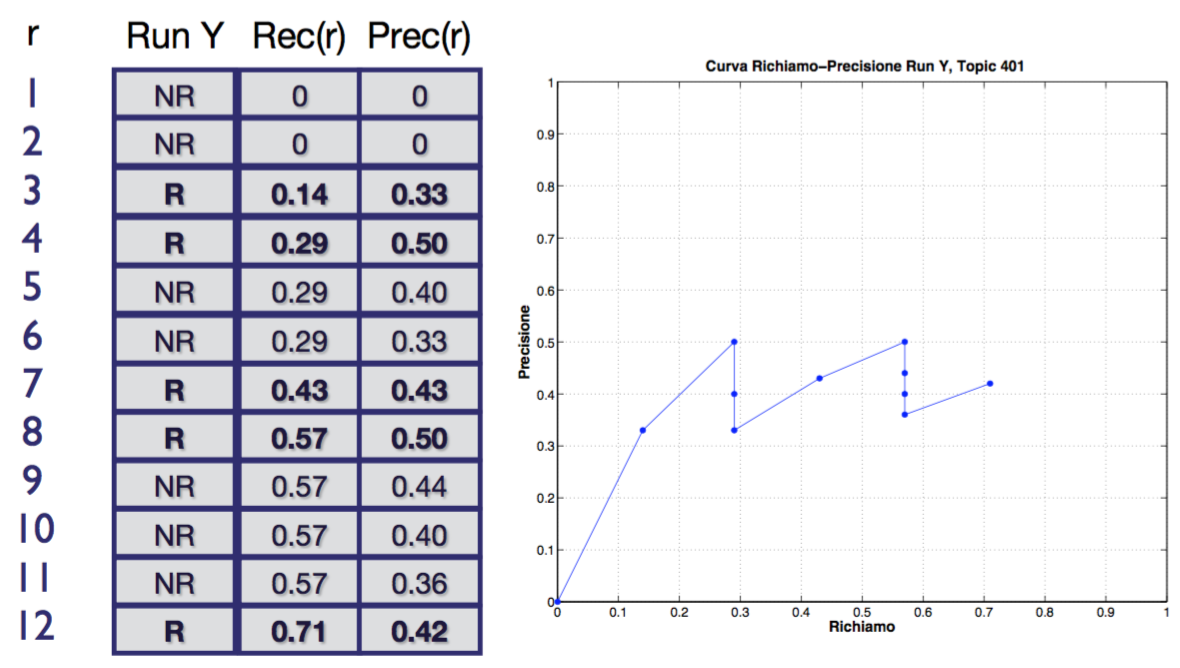
\includegraphics[width=0.6\textwidth]{images/l15-fig-4.png}
	\caption{Esempio della curva richiamo-precisione.}
\end{figure}

Ovvero per ogni livello di rango vengono calcolate la precisione e il richiamo con cut-off a quel livello.

Questa curva però ha un sacco di problemi, perché intanto non è una funzione, inoltre non è possibile utilizzarla per comparare due run distinte. C'è poi anche da tenere in considerazione che uno stesso sistema può produrre run diverse.

Una variante è la curva \textbf{interpolata}: una curva simile che viene ottenuta considerando 11 punti fissi di richiamo (\textbf{11-point recall-precision}):

$$
rp \in \{ 0, 0.1, 0.2, \ldots 1 \}
$$

e viene calcolata come 

$$
IP_{rp} = \max_{1 \leq r \leq N | Rec(r) \geq rp} Prec(r)
$$

ovvero, ad ognuno dei punti dell'insieme $rp$ viene associato il più alto valore di precisione ottenuto sui primi $r$ valori della run che hanno un richiamo maggiore del punto.

\begin{figure}[htbp]
	\centering
	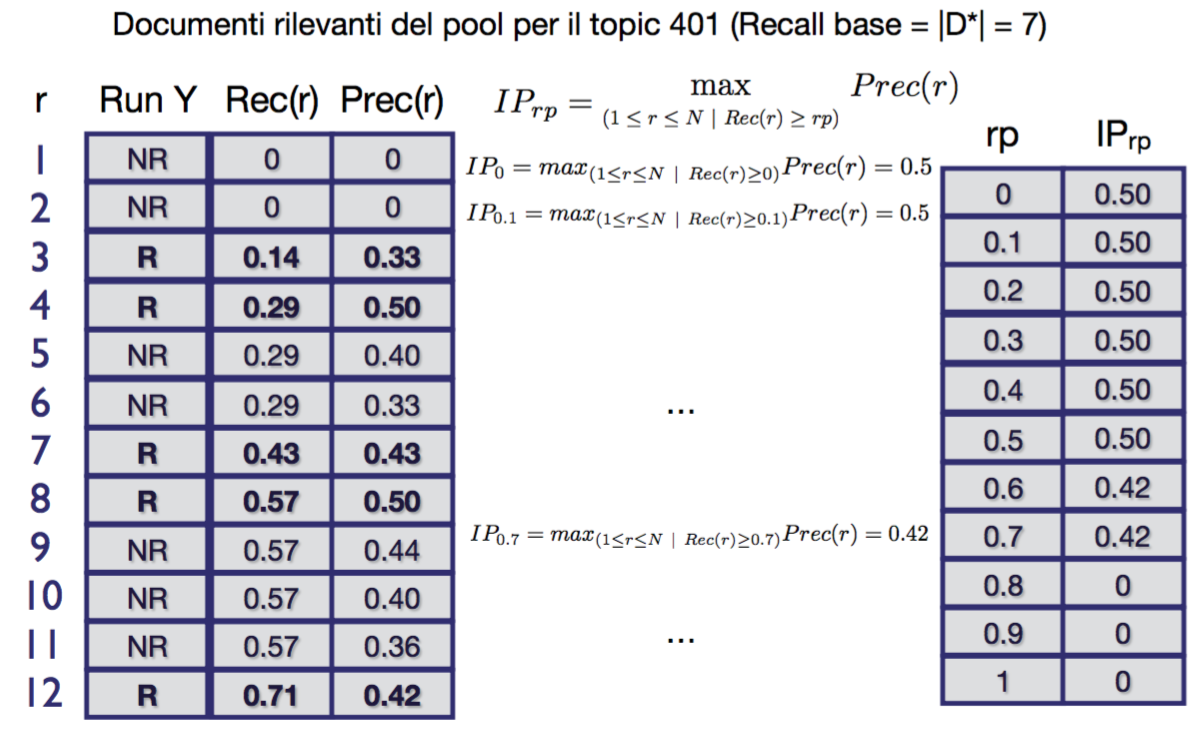
\includegraphics[width=0.6\textwidth]{images/l15-fig-5.png}
	\caption{Esempio di calcolo della curva richiamo-precisione interpolata.}
\end{figure}

\begin{figure}[htbp]
	\centering
	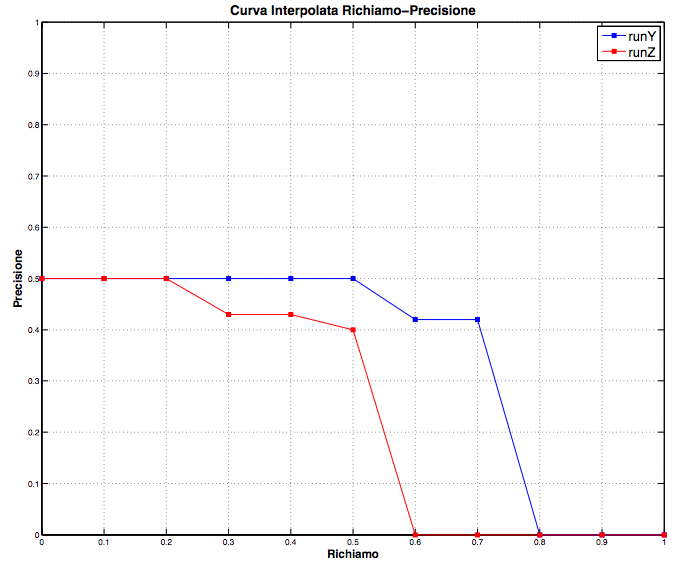
\includegraphics[width=0.4\textwidth]{images/l15-fig-6.png}
	\caption{Esempio di curva richiamo-precisione interpolata.}
\end{figure}


Questa curva va bene per giudicare ad occhio quale delle due curve va meglio, però si può fare di più utilizzando l'11-\textbf{Point Average Precision} che effettua la media di tutti i valori di precisione interpolata calcolati.

$$
\text{11pt-AP} = \frac{\sum_{rp\in\{0,0.1,\ldots 1 \}}IP_{rp}}{11}
$$

C'è però un'effetto indesiderato perché la precisione a valori alti di richiamo ha lo stesso peso di quelli a livelli bassi.

Tipicamente si usa quindi l'\textbf{Average Precision} che è la misura attualmente più utilizzata.

Dato un topic $t \in T$, una recall base $RB_t$, $REL =\{ nr, r \}$ e una run $r_t$ di lunghezza $N$ tale che:

$$
\forall i \in [1, N], \tilde{r}_t = \begin{cases}
0 \quad &\text{se } \hat{r}_t[i] = nr \\
1 \quad &\text{se } \hat{r}_t[i] = r \\
\end{cases}
$$

l'average precision è quindi definita come:

$$
AP = \frac{1}{RB_t}\sum\limits_{k=1}^{N}\tilde{r}_t[k]\frac{\sum\limits_{h=1}^{k} \tilde{r}_t[h]}{k}
$$

Le misure di questo tipo prendo il nome di \textbf{top heavy} perché danno più peso ai documenti rilevanti in posizioni alte del rank.

\begin{figure}[htbp]
	\centering
	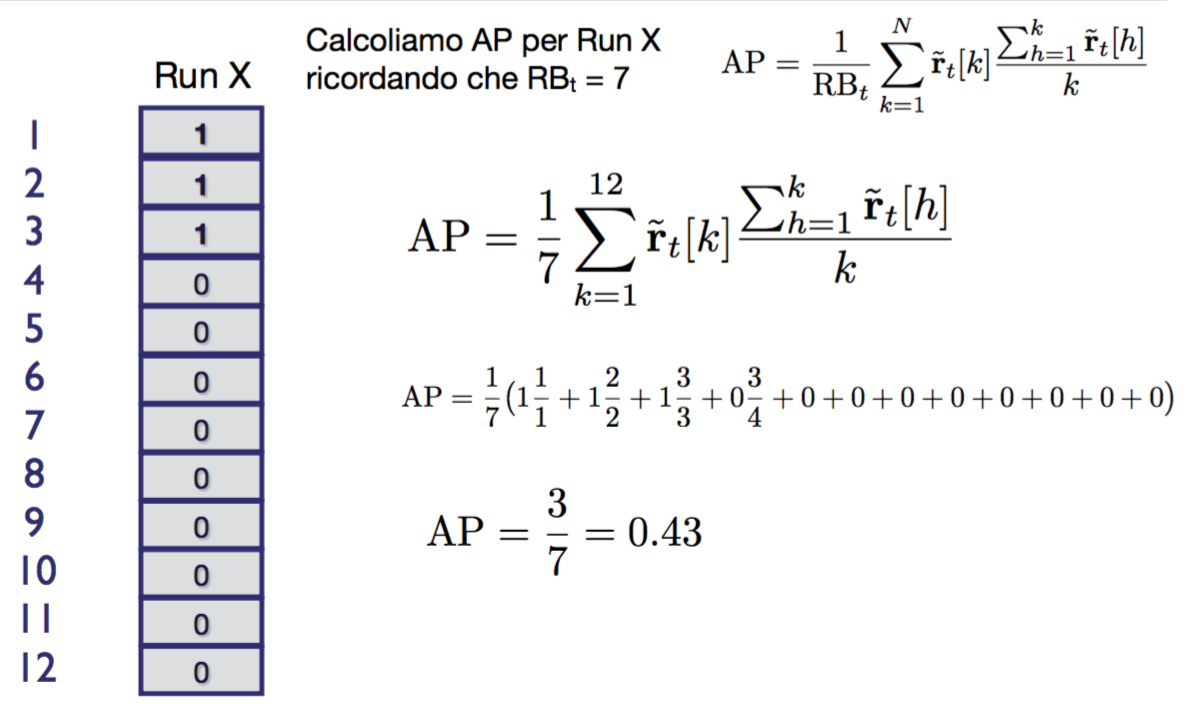
\includegraphics[width=0.7\textwidth]{images/l15-fig-7.png}
	\caption{Esempio di calcolo di Average Precision.}
\end{figure}

\section{Valutazione di un sistema su più topic}

Le misure viste finora valutano la singola run su un topic, ma tipicamente le campagne di valutazione sono fatte su 50 o 100 topic.

L'idea base è quella di fare la media aritmetica delle run sui singoli topic. Si parla quindi di \textbf{Mean Average Precision} (\textbf{MAP}). Detta anche la \textit{media media precisione}.

$$
MAP(R) = \frac{\sum_{t\in T}AP(r_t)}{|T|}
$$

Tipicamente è una brutta idea fare la media di una misura che dipende dalla recall base. Ma nel campo di valutazione dell'IR, AP è una misura che piace e quindi si fa comunque la media. 

Quindi \textbf{MAP} bene, \textbf{R-prec-media} male.

% !TEX encoding = UTF-8
% !TEX program = pdflatex
% !TEX root = InformationRetrieval.tex
% !TEX spellcheck = it-IT

% 2 Dicembre 2016

\subsection{BM25}

La strada che ha portato ad ottenere il BM25 è stata molto lunga ed è iniziata negli anni 70.

\subsubsection{L'inizio del percorso}

Ripartendo dal BIM, la probabilità che un documento sia rilevante per una query può essere stimata con: 

\begin{align}
P(\rel | d,q) &\propto_q \frac{P(d|\rel, q)}{P(d| \notrel, q)} \\ 
&\approx \prod_{i \in V} \frac{P(TF_i=tf_i|rel,q)}{P(TF_i=tf_i | \notrel, q)} \underbrace{\frac{P(\rel|q)}{P(\notrel |q )}}_{\text{costante per tutti i documenti}} \nonumber  \\
&\approx \prod_{i \in V} \frac{P(TF_i = tf_i|\rel,q)}{P(TF_i=tf_i|\notrel,q)}\nonumber \\
&\approx \prod_{i \in q} \frac{P(TF_i = tf_i|\rel)}{P(TF_i=tf_i|\notrel)}
\end{align}

Da notare che la formula utilizza una variabile aleatoria diversa, per distinguere i passi che hanno portato al BM25 dalla formulazione del BIM. $TF_i$ è una variabile aleatoria che rappresenta la frequenza del termine $i$ all'interno del documento $d$. Il valore della frequenza per un dato termine è $tf_i$. $V$ continua invece ad essere il vocabolario.
Possono inoltre \textbf{limitare la produttoria} a tutti i termini delle query $i \in q$ e rimuovere il condizionamento, facendo l'ipotesi che tutti i termini che non compaiono nella query hanno la stessa probabilità di apparire sia nei rilevanti che non rilevanti. Quindi posso evitare di considerarli, perché il rapporto vale 1.

La produttoria non può essere calcolata perché lavora con numero troppo piccoli, quindi si considerano i logaritmi:

\begin{align}
P(\rel | d,q) &\propto_q \sum_q \underbrace{\log \Big(  \frac{P(TF_i=tf_i | \rel)}{P(TF_i=tf_i | \notrel )} \Big)}_{U_i(tf_i)} \\ 
&= \sum\limits_q U_i(tf_i) \\
&= \sum_{q,tf_i > 0} U_i(tf_i) + \sum_{q,tf_i = 0} U_i(0)
\end{align}

Nell'ultimo passaggio la sommatoria viene scomposta in modo da separare i termini con $tf_i > 0$ da quelli con $tf_i = 0$.

Nel procedimento del paper c'è un passaggio strano che l'autore l'ha motivato così: tutti i modelli prima del '74 partono dall'idea che ci sono le frequenze dei termini da sommare per calcolare lo score del documento, ma non viene mai presa in considerazione l'assenza dei termini.
Questo per motivi di efficienza perché nel '74 la potenza di calcolo era ridotta.

Quindi viene fatto il giochino di sommare e togliere la stessa quantità, in modo da poter raggruppare le sommatorie in un altro modo, per ottenere dei calcoli più semplici da fare.

\begin{align}
P(\rel | d,q) &\propto_q \sum_{q,tf_i > 0} U_i(tf_i) + \sum_{q,tf_i = 0} U_i(0) \nonumber \\
&= \sum_{q,tf_i > 0} U_i(tf_i) + \underbrace{\sum_{q,tf_i = 0} U_i(0) + \sum_{q, tf > 0} U(0)}_{\text{possono essere raggruppate}} - \sum_{q, tf > 0} U_i(0) \nonumber \\
&= \sum_{q, tf>0} \Big( U_i(tf_i) - U_i(0) \Big) + \underbrace{\sum_q U_i(0)}_{= 0}  \nonumber \\
&\propto_q \sum_{q, tf>0} \Big( U_i(tf_i) - \underbrace{U_i(0)}_{\text{costante per tutti i documenti}} \Big)
\end{align}

Quindi per calcolare la probabilità della rilevanza possono considerare solamente i termini che compaiono sia nella query che nei documenti.

Andando a espandere $U_i$ otteniamo:

\begin{align}
P(\rel | d,q) &\propto_q \sum_{q, tf>0} \Big( U_i(tf_i) - U_i(0) \Big) \nonumber \\
&\propto_q \sum_{q, tf>0} \log\frac{ P(TF_i = tf_i | \rel) P(TF_i = 0 | \notrel) }{P(TF_i = tf_i | \notrel) P(TF_i = 0 | \rel)} \label{eq:basic-prob}\\
&= \sum_{q, tf>0} W_i(tf_i)
\end{align}

Ottenendo così la formula basilare per andare a pesare la presenza di un termine della query all'interno di un documento, tenendo conto della frequenza con cui compare nel documento.

Dato che si tratta di un formulone, si può ridurre a:

\begin{align}
W_i(tf_i) &= \log\frac{ P(TF_i = tf_i | \rel) P(TF_i = 0 | \notrel) }{P(TF_i = tf_i | \notrel) P(TF_i = 0 | \rel)} = \log \frac{p_{tf_i} u_0}{u_{tf_i} p_0} \label{eq:basic-weight}
\end{align}

\noindent dove:

\begin{itemize}
\item $p_{tf_i} =  P(TF_i = tf_i | \rel) $ ovvero la probabilità che il termine $i$ \textbf{compaia} $tf_i$ volte nel documento, dato che il documento è \textbf{rilevante}.
\item $p_0 = P(TF_i = 0 | \rel) $ ovvero la probabilità che il termine $i$ \textbf{non compaia} nel documento, dato che il documento è \textbf{rilevante}.
\item $u_{tf_i} =  P(TF_i = tf_i | \notrel) $ ovvero la probabilità che il termine $i$ \textbf{compaia} $tf_i$ volte nel documento, dato che il documento è \textbf{non rilevante}.
\item $u_0 = P(TF_i = 0 | \notrel) $ ovvero la probabilità che il termine $i$ \textbf{non compaia} nel documento, dato che il documento è \textbf{non rilevante}.
\end{itemize}

Da notare che $p_0$ è diverso da $(1-p_{tf_i})$ perché $p_0$ modella l'assenza del termine e non il complemento di $p_{tf_i}$.

Nel caso di un modello con le variabili binarie, ovvero in cui $tf_i$ è 1 o 0, ci riconduciamo a qualcosa di simile al BIM, perché andando ad utilizzare i valori binari nell'equazione \ref{eq:basic-prob} otteniamo:

\begin{align}
P(\rel | d,q) &\propto_q \sum_{q, tf>0} \log\frac{ P(TF_i = 1 | \rel) P(TF_i = 0 | \notrel) }{P(TF_i = 1 | \notrel) P(TF_i = 0 | \rel)} \\
&= \sum_{q, tf>0} \log \Big(  \frac{p_i (1-\varphi_i)}{\varphi_i(1-p_i)} \Big)
\end{align}

Da notare che $\varphi_i$ è la $q_i$ del BIM, viene cambiato il simbolo per non fare confusione con la $q$ della query. 
Si ottiene quindi lo stesso risultato ottenuto dal modello binario utilizzando la teoria bayesiana.

\subsubsection{Il modello 2-Poisson}

Data una query ci sono termini che sono abbastanza infrequenti, che appaiono poche volte e termini che compaiono molto più frequentemente\footnote{Deriva da un'osservazione sperimentale}. Il tutto senza considerare le stop-word.

Si è osservato che la distribuzione di questi termini segue la distribuzione di Poisson:

$$
\mathcal{P}(\lambda) = \frac{\lambda^k}{k!}e^{-\lambda}
$$

Dove $k$ è un valore dato, che nel nostro caso rappresenta la frequenza del termine e $\lambda$ è un parametro della distribuzione. Il parametro $\lambda$ va ad influenzare la media della distribuzione.

La probabilità di una variabile aleatoria $X$ che segue la distribuzione di Poisson viene quindi calcolata con

$$
P(X = x) \frac{\lambda^x}{x!}e^{-\lambda}
$$

Viene quindi assunto che l'occorrenza dei termini sia casuale ma che si distribuisca attorno una certa media.

Da qui è nato il modello 1-Poisson, che calcola la probabilità che un termine $i$ appaia con una certa frequenza con

$$
P(TF_i = tf_i) \approx \frac{\hat{\lambda}^{tf_i}}{{tf_i}!}e^{-\hat{\lambda}}
$$

\noindent dove $\hat{\lambda} = \cfrac{c_i}{N}$, ovvero $\lambda$ viene stimato utilizzando la frequenza media del termine $i$ all'interno della collezione ($c_i$ è la collection frequency del termine e $N$ è il numero di documenti presenti nella collezione).
Questo però non andava benissimo e quindi si è passati al 2-Poisson model.

Si è osservato che i termini possono essere divisi in due gruppi: un gruppo che contiene i termini che appaiono poche volte $\mu$ (e che seguono una distribuzione con $\lambda = \mu \approx 1$) e l'altro che contiene quelli che compaiono molte volte $\lambda > \mu$. 

L'ipotesi che è stata fatta è che la probabilità di osservare un termine generico in un documento è data da una "\textit{mistura}" di queste due distribuzioni. Ovvero preso un documento a caso, la probabilità di osservare un termine dipende dalle due distribuzioni $\mu$ e $\lambda$.

C'è poi il concetto di \textbf{éliteness}, fissato un termine all'interno di un documento, tanto più frequente sarà quel termine, tanto più d'élite sarà quel documento per il concetto rappresentato dal termine. 
Quindi, tanto più frequente è un termine all'interno del documento, tanto più il documento è d'élite rispetto al concetto descritto dal termine e di conseguenza, se il termine compare anche nella query, la probabilità che il documento sia anche rilevante aumenta.

Il modello 2-Poisson si basa quindi su due distribuzioni, che modellano la probabilità che un termine che appare con una certa frequenza nel documento sia d'élite o meno:

\begin{align}
a_{tf} &= P(TF_i = tf_i | E_i = \elite) = \frac{\lambda^{tf_i}}{{tf_i}!}e^{-\lambda}\\
n_{tf} &= P(TF_i = tf_i | E_i = \notelite) = \frac{\mu^{tf_i}}{{tf_i}!}e^{-\mu}
\end{align}

La distribuzione di un termine in un documento segue dipende quindi da entrambe le distribuzioni, perché non si sa se quel termine è d'élite nel documento o meno, ovvero:

$$
P(TF_i = tf_i) = \pi \frac{\lambda^{tf_i}}{{tf_i}!}e^{-{\lambda}} + (1 - \pi) \frac{\mu^{tf_i}}{{tf_i}!}e^{-\mu}
$$

\noindent dove $\pi$ è la probabilità che il documento sia d'élite e tipicamente non è nota.

Il tutto per dire che per pesare un termine bisogna tenere in considerazione sia la rilevanza del documento che l'éliteness ed entrambe le caratteristiche sono influenzate dalla frequenza del termine. 

Inoltre, dato che l'éliteness e la rilevanza sono due cose distinte, ci possono essere dei documenti d'élite per un certo argomento ma che non sono rilevanti per la query.
Si ha poi che un documento è d'élite per un determinato termine se questo termine è molto presente, senza prendere in considerazione la rilevanza.
Quindi:

\begin{align}
P(TF_i = tf_i | \rel) &= P(tf_i | E_i = \elite)P(E_i = \elite | \rel) + P(tf_i |E_i = \notelite)P(E = \notelite | \rel) \\
P(TF_i = tf_i | \notrel) &= P(tf_i | E_i = \elite)P(E_i = \elite | \notrel) + P(tf_i |E_i = \notelite)P(E_i = \notelite | \notrel) 
\end{align}

Si può quindi abbreviare con

\begin{itemize}
	\item $p_i' = P(E_i = \elite | \rel)$
	\item $q_i' = P(E_i = \elite | \notrel)$
\end{itemize}

e andare a pesare il termine con la formula \ref{eq:basic-weight}, sostituendo le due formule sopra riportate:

\begin{align}
W_i(tf_i) &=  \log\frac{ P(TF_i = tf_i | \rel) P(TF_i = 0 | \notrel) }{P(TF_i = tf_i | \notrel) P(TF_i = 0 | \rel)} \\
&= \log \frac{
\big(p_i'\lambda^{tf_i}e^{-\lambda} + (1-p_i')\mu^{tf_i}e^{-\mu}\big)\big(q_i'e^{-\lambda} + (1-q_i')e^{-\mu}\big)
}{
\big(q_i'\lambda^{tf_i}e^{-\lambda} + (1-q_i')\mu^{tf_i}e^{-\mu}\big)\big(p_i'e^{-\lambda} + (1-p_i')e^{-\mu}\big)
} \label{eq:wtf}
\end{align}


C'è quindi il problema della stima di questi 4 parametri, nessuno dei quali può essere stimato osservando i documenti a disposizione, perché l'éliteness è una variabile nascosta. \`E stata questa la critica degli autori del BM25 verso il 2-Poisson. Tuttavia le osservazioni alla base di questo modello si sono rivelate essere corrette.


\subsubsection{Approssimazioni del 2-Poisson}

Risulta quindi necessario utilizzare un'approssimazione della funzione di peso del 2-Poisson.
Per fare questa approssimazione si può osservare che:

\begin{enumerate}
	\item Se $tf_i = 0$, anche $W_i(0) = 0$.
	\item La funzione cresce in monotonicamente come $tf_i$.
	\item C'è un massimo asintotico.
	\item Il massimo è simile al sistema di pesi del BIM:
	$$
	\lim\limits_{tf_i \to \infty} W_i^{elite}(tf_i) = \log \frac{p_i'(1-q_i')}{q_i'(1-p_i')}
	$$
\end{enumerate}

\begin{figure}[htbp]
	\centering
	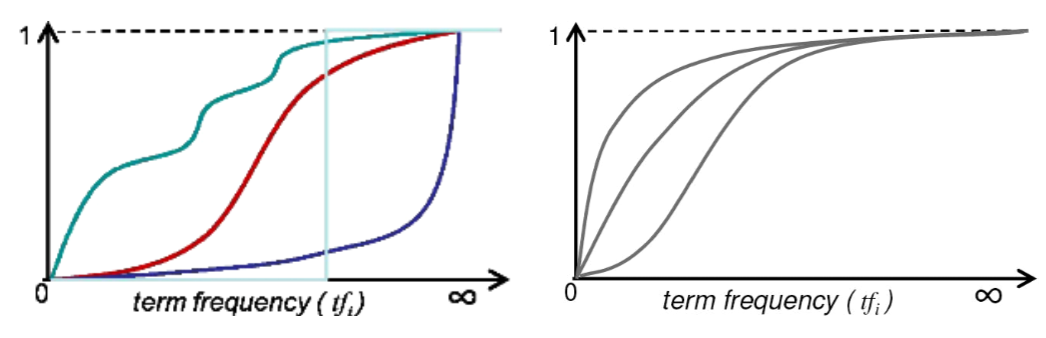
\includegraphics[width=0.9\textwidth]{images/l19-fig-1.png}
	\caption{A sinistra: alcune possibile funzioni di saturazione che sono compatibili con i 4 punti dell'elenco. A destra: funzioni di saturazione generate dal 2-Poisson.}
\end{figure}

Quindi se l'éliteness fosse osservabile, sarebbe possibile trattarla come un attributo binario e utilizzare la stessa funzione di pesatura del BIM.
Questo a livello asintotico ha senso. Perché dato che l'unica associazione tra $tf_i$ e la rilevanza passa attraverso l'éliteness, la miglior informazione che possiamo sperare di ottenere da un termine è che il documento è d'élite per quel termine. In realtà la nostra informazione riguardo questo score è probabilistica, e quindi il peso del termine viene ridotto secondo la questa probabilità. Questo comportamento prende il nome di \textbf{saturazione}.
Da notare che l'unico caso in cui non vale la saturazione è quando la rilevanza e l'éliteness coincidono, ottenendo un limite infinito e rendendo il peso del termine lineare rispetto alla frequenza, come avviene con $tf\cdot idf$.

Gli autori di BM25 hanno quindi deciso di approssimare l'effetto dell'éliteness utilizzando la curva

\begin{align}
\frac{tf_i}{k + tf_i} \ref{eq:raw}
\end{align}

\noindent per qualche $k > 0$.

L'approssimazione utilizzata inizialmente per l'equazione \ref{eq:wtf} è quindi

\begin{align*}
W_i(tf_i) &= \frac{tf_i}{k + tf_i}  w_i^{RSJ} \\
&=\frac{tf_i}{k + tf_i}  \log \bigg( \frac{N_{t_iR} + 0.5}{N_R - N_{t_iR} + 0.5} \frac{N - N_R - N_{t_i} + N_{tR + 0.5}}{N_{t_i} + N_{t_iR} +0.5} \bigg)
\end{align*}

\noindent dove $w_i^{RSJ}$ deriva dall'equazione \ref{eq:wrsj} ed è una versione semplificata del BM15.

Tutto questo funziona se assumiamo che i documenti hanno la stessa lunghezza perché consideriamo quante volte compare un termine all'interno di un documento, senza preoccuparci del numero totale di termini. Ovviamente non possiamo fare tale assunzione.

I primi modelli che tenevano in considerazione la lunghezza del documento, modificavano la frequenza del termine dividendola per la lunghezza del documento $dl$, effettuando una normalizzazione della frequenza.

$$
dl = \sum\limits_{i \in V} tf_i
$$

\noindent Si è quindi ottenuto un BM-qualcosa.

$$
W_i(tf_i) = \frac{\cfrac{tf_i}{dl}}{k + \cfrac{tf_i}{dl}}  w_i^{RSJ}
$$

Infine nel '96 sono stati accorpati il BM11 e BM15 si è ottenuto il BM25. Ci sono arrivati osservando che i documenti più corti avevano una maggior probabilità di essere recuperati. 
Hanno quindi scelto di bilanciare l'effetto della lunghezza aumentando leggermente la probabilità di recuperare un documento più lungo della media e diminuendo la probabilità per quelli sotto la media.

Questo è stato fatto andando a normalizzare la $tf_i$ con

$$
B = (1-b)+ b\frac{dl}{avgdl}
$$

\noindent dove $avgdl$ è la lunghezza media dei documenti della collezione.
Quindi se $b=1$ viene fatta la normalizzazione completa, dando maggiore probabilità di retrieval ai documenti corti mentre se $b=0$ viene data maggiore probabilità di retrieval ai documenti lunghi, in quanto non viene fatta la normalizzazione.

\begin{figure}[htbp]
	\centering
	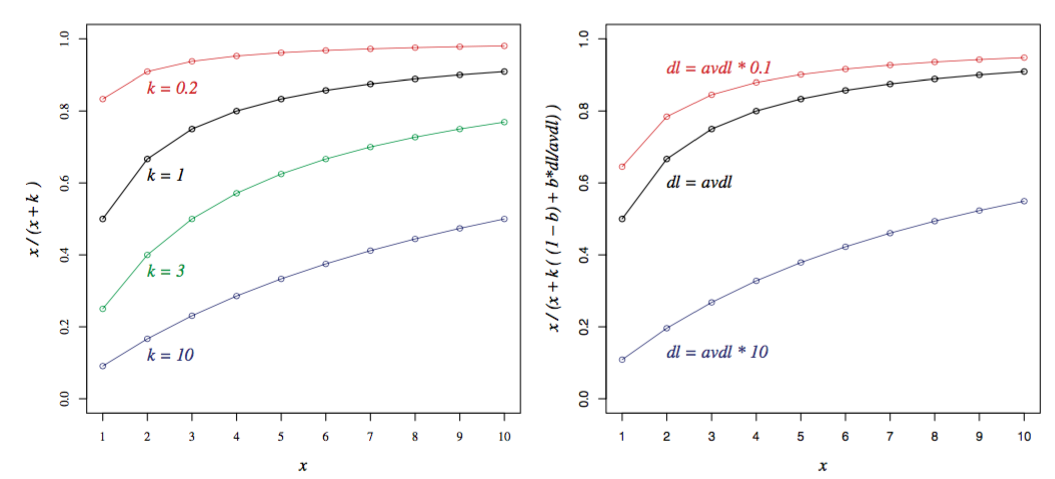
\includegraphics[width=0.9\textwidth]{images/l19-fig-2.png}
	\caption{A sinistra: funzioni di saturazione generate con l'equazione \ref{eq:raw}. A destra: funzioni di saturazione generate normalizzando $tf_i$ con $B$ ($k=1, b=0.5$).}
\end{figure}


Mettendo tutto assieme si ottiene il BM25 semplificato: 

\begin{align}
\boxed{
	W_i^{BM25}(tf_i) = \frac{tf_i}{k_1\bigg((1-b)+ b\cfrac{dl}{avgdl}\bigg) + tf_i } w_i^{RSJ}
}
\end{align}

Tipicamente come parametri viene utilizzato $k_1=1.5$ e $b=0.75$, tuttavia possono essere ottimizzati ad hoc in modo sperimentale.
Tuttavia questo modello avrebbe un'ulteriore componente che tiene conto della frequenza dei termini della query. Tale fattore viene però tenuto tipicamente uguale a 1, perché salvo rari casi la frequenza dei termini nella query è sempre 1, salvo rari casi in cui la query è rappresentata da un documento.
C'è poi un'altra variante che sostituisce moltiplica il numeratore per $k_1+1$.

La versione "completa" del BM25 è quindi:

\begin{align}
W_i^{BM25}(tf_i) = \frac{(k_1+1)tf_i}{k_1\bigg((1-b)+ b\cfrac{dl}{avgdl}\bigg) + tf_i } \times \frac{(k_3+1)qtf_i}{k_3 + qtf_i} \times w_i^{RSJ}
\end{align}

\noindent Da notare che manca il termine $k_2$, questo perché era un parametro del modello che c'era una volta, ma tutti gli esperimenti che hanno visto che i risultati migliori si trovano con $k_2=0$ e quindi non viene più considerato.

\begin{itemize}
\item non posso chiedervi di  calcolare delle formule con bm25

\item posso chiedervi che data, una collezione di documenti con tf e rilevanza, calcolare qual'è il documento più rilevante (calcolo di log p/q (1-q)/(1-p), con numeri appropriati in modo che non serva la calcolatrice.

\item posso chiedervi le ipotesi di partenza da 2-poisson a bm25. Interessa il ragionamento. Dato il formulone generale, quali sono le ipotesi semplificative che permettono di arrivare a bm25.
\end{itemize}











% !TEX encoding = UTF-8
% !TEX program = pdflatex
% !TEX root = InformationRetrieval.tex
% !TEX spellcheck = it-IT
% 22 Dicembre 2016

\todo[inline]{Recuperare lezione 22 dicembre - Web search}
% !TEX encoding = UTF-8
% !TEX TS-program = pdflatex
% !TEX root = computabilità e algoritmi.tex
% !TEX spellcheck = it-IT
\chapter{Algoritmi multithread}\label{algoritmi-multithread}

Finora abbiamo visto solamente algoritmi sequenziali, ma il progresso ha fornito la possibilità di eseguire algoritmi paralleli.

Il problema è che non c'è un modello di calcolo preciso. 
Tipicamente ci sono più processori con della memoria condivisa, oppure ci sono dei cluster composti da processori, ognuno con la propria memoria che comunica con altri cluster per condividere i dati.

Noi ci limiteremo al caso con più processori con memoria condivisa.

In questo caso il lavoro deve essere distribuito tra i vari processori, utilizzando dei \textbf{thread}, dei processi logici che vengono assegnati ai vari processori.

Tipicamente una volta che il thread è stato avviato, questo non viene fermato e rimane in esecuzione su quel processore fino alla fine (\textbf{thread statico}).

La gestione dei thread viene effettuata in modo automatico (\textbf{threading dinamico}) perché lasciarla allo sviluppatore è troppo pericoloso. 
Con questa modalità, il programmatore può specificare quali parti del programma possono essere eseguite in parallelo, la suddivisione del programma in thread viene lasciata alla \textbf{piattaforma parallela} i quali vengono poi assegnati ai vari processori.

L'assegnazione viene effettuata con uno scheduler che cerca di bilanciare il lavoro svolto dai vari processori.

\section{Il primo algoritmo parallelo}\label{il-primo-algoritmo-parallelo}

Come notazione per lo pseudo codice utilizzeremo:

\begin{itemize}
\item
  \textbf{spawn}: posta davanti ad un istruzione indica che questa può essere eseguita in parallelo rispetto al resto del programma. In altre parole segnala che l'istruzione può essere eseguita su un altro thread.
\item
  \textbf{sync}: segnala che è necessario aspettare la terminazione di tutti i thread attivati con spawn.
\item
  \textbf{parallel}: specifica che il corpo di un ciclo \texttt{for} può essere eseguito in modo parallelo.
\end{itemize}

L'istruzione \textbf{spawn} non obbliga il sistema ad eseguire il codice in parallelo, è il sistema che sceglie se conviene o meno.

Se da un programma parallelo togliamo tutte queste istruzioni, otteniamo un classico programma sequenziale.

\subsection{Fibonacci ricorsivo}\label{fibonacci-ricorsivo}

\begin{breakablealgorithm}
\caption{P-Fib: fibonacci in versione parallela}
\begin{algorithmic}[1]
\Function{P-Fib}{n}
\If{$n \leq 1$}
    \State \Return $n$
\EndIf
\State $x \gets \textbf{ spawn } \textsc{P-Fib}(n-1)$ 
\State $y \gets \textsc{P-Fib}(n-2)$
\State $\textbf{sync}$
\State \Return $ x + y$
\EndFunction
\end{algorithmic}
\end{breakablealgorithm}

La complessità per la \textbf{versione sequenziale} di questo codice è proporzionale al numero ritornato dalla funzione, il quale cresce esponenzialmente.

\subsection{Grafo di computazione}\label{grafo-di-computazione}

L'esecuzione di un algoritmo multithread può essere rappresentata con un DAG.

Come prima cosa è necessario individuare gli \textbf{strand} ovvero le porzioni di codice che vengono eseguite in modo sequenziale.

Come notazione per il grafo viene utilizzato:

\begin{itemize}
\item
  \textbf{nero} o un pallino pieno per indicare uno strand.
\item
  \textbf{grigio} o un pallino con una crocetta per indicare la porzione di codice che c'è tra una \textbf{spawn} e una \textbf{sync}.
\item
  \textbf{bianco} o un pallino vuoto per indicare l'istruzione di
  ritorno per un thread (o funzione).
\end{itemize}

\begin{figure}[htbp]
\centering
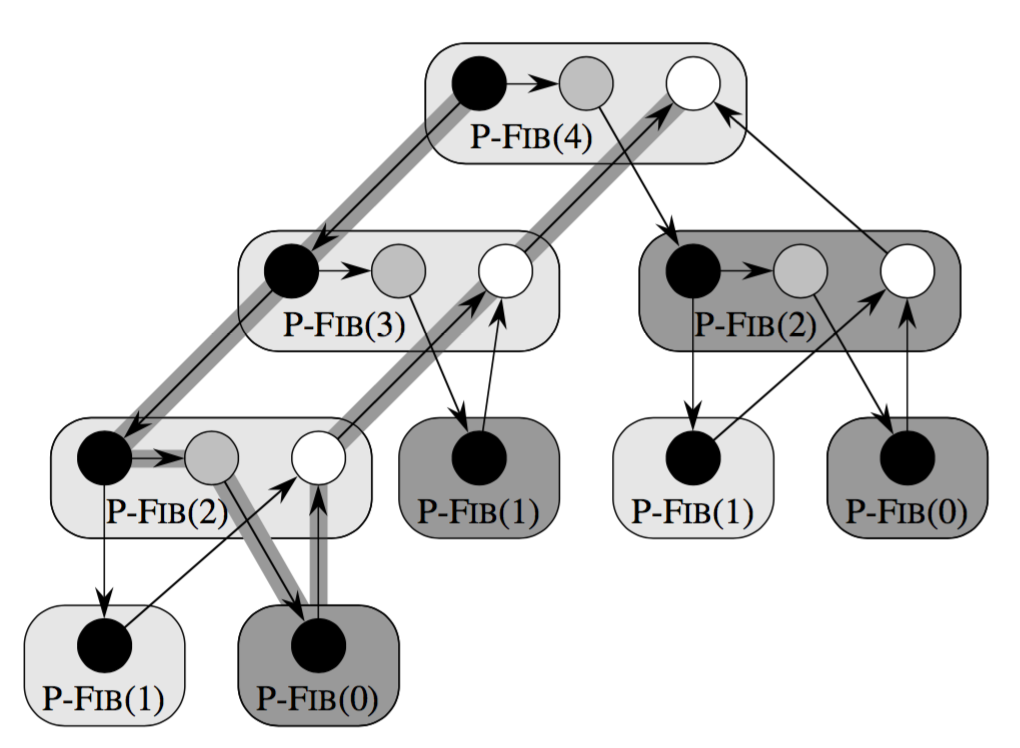
\includegraphics[width=.6\textwidth]{./notes/immagini/l24-fig1.png}
\caption{DAG per \textsc{P-Fib}(4)}
\end{figure}

(sistemare immagine, aggiungere la versione alternativa, spiegare gli
archi)

\subsection{Metriche per la complessità}\label{metriche-per-la-complessituxe0}

Per quanto riguarda la complessità asintotica possiamo considerare che l'esecuzione di uno strand avvenga in tempo costante.

Vengono poi distinte due misure: il \textbf{lavoro} ovvero il numero di strand e la \textbf{durata} (span) che è la lunghezza del cammino massimo (critico) del DAG, ovvero il numero di strand che devono per forza essere eseguiti in sequenza.

Nell'esempio di Fibonacci, il lavoro è 17 e la durata è 8 unità di tempo.

Ovviamente se l'algoritmo viene eseguito in modo sequenziale, il lavoro coincide con la durata ($T_1$). 
Se invece si hanno a disposizione infiniti processori, la durata è il tempo minimo richiesto ($T_\infty$). 

Infine, se si hanno a disposizione \emph{P} processori, valgono:

\begin{itemize}
	\item \textbf{legge del lavoro}: $T_P \geq \frac{T_1}{P}$
	\item \textbf{legge della durata}: $T_P \geq T_\infty$.
\end{itemize}

Lo \textbf{speedup} di un algoritmo misura quanto viene velocizzato l'algoritmo utilizzando \emph{P} processori:

$$\textbf{speedup} = \frac{T_1}{T_P} \leq P$$

Se lo speedup è molto più piccolo di \emph{P} non è conveniente aumentare il numero di processori.

Lo speedup viene detto \textbf{lineare} se

$$\frac{T_1}{T_P} = O(P)$$

e \textbf{perfetto} se

$$\frac{T_1}{T_P}  = P$$

Un'altra misura è data dal \textbf{parallelismo} che è il rapporto tra $T_1$ e $T_\infty$ e misura il lavoro medio che può essere eseguito in parallelo, fornendo un limite superiore per lo speedup.

Il parallelismo fornisce anche un limite allo speedup perfetto, ovvero supponendo di avere un numero di processori molto più grande del parallelismo:

$$P >> \frac{T_1}{T_\infty} \quad \text{ allora } \quad \frac{T_1}{T_P} << P$$

Il \textbf{lasco} del parallelismo viene definito come

$$\frac{T_1/T_\infty}{P}$$

ovvero di quanto il parallelismo è maggiore del numero di processori.

Se il lasco è minore di 1, si ha che 

$$\frac{T_1}{T_P} \leq \frac{T_1}{T_\infty} < P$$

quindi si ha che lo speedup non potrà mai essere perfetto. 

Se invece il lasco è maggiore di 1, ci si può avvicinare allo speedup perfetto.

\subsection{Lo scheduling dei thread}\label{lo-scheduling-dei-thread}

L'ordine ottimo che minimizza la durata dell'algoritmo è dato dall'ordinamento topologico del DAG, il quale non è noto a priori.

Lo scheduler più semplice è quello \textbf{goloso}, il quale assegna il maggior numero possibile di strand ai processori che ha a disposizione. Se ci sono più strand che thread, la scelta degli strand da assegnare viene fatta casualmente.

Se tutti i thread sono in esecuzione si verifica un passo \textbf{completo} ovvero tutti i processori stanno lavorando. 
Se non ci sono strand a sufficienza per tenere impegnati tutti i processori si ha un passo \textbf{incompleto}. 
Si ottiene così una durata che è pari alla somma dei passi completi e di quelli incompleti.

\subsubsection{Durata di un algoritmi con lo scheduler goloso}

Usando lo scheduler goloso è sempre vero che:

$$T_P \leq \frac{T_1}{P} + T_\infty$$

Il numero di passi completi è $\leq \frac{T_1}{P}$, perché se per assurdo non lo fosse, verrebbe eseguito più lavoro di quanto necessario:

$$
\underbrace{P \cdot \bigg(\bigg\lfloor \frac{T_1}{P}\bigg\rfloor +1 \bigg)}_{\text{lavoro svolto dai passi completi assumendo di farne più del necessario}} = P \bigg( \frac{T_1}{P} - (T_1 \mod P) +1 \bigg) = T_1 + P > T_1
$$
\todo[inline]{Verificare che sia corretto, nel libro fa un passo in più e Colussi ha fatto un giro strano}
 il che è assurdo.

Dopo aver eseguito un certo numero di passi completi, verrà eseguito un passo incompleto, quando questo succederà il DAG della computazione sarà un grafo $G'$ che avrà un numero di nodi iniziali (senza dipendenze) minore di \emph{P}, perché il passo è incompleto. 
Per forza di cose, uno di questi nodi appartiene al cammino critico e verrà eseguito, diminuendo di 1 la lunghezza di tale cammino. 
Dal momento che all'inizio la lunghezza del cammino è $T_\infty$, possono esserci al massimo
$T_\infty$ passi incompleti.

Quindi, dato che un passo può essere o completo o incompleto, la durata dell'algoritmo con $ P $ processori è limitata dal numero di passi, ovvero:

$$
T_P \leq \underbrace{\bigg\lfloor \frac{T_1}{P}\bigg\rfloor}_{\text{massimo numero di passi completi}} + \underbrace{T_\infty}_{\text{massimo numero di passi incompleti}}
$$

Questo tipo di scheduler funziona sufficientemente bene dal momento che nel caso peggiore richiede il doppio del tempo rispetto alla schedulazione ottima effettuata conoscendo a priori il DAG, ovvero lo scheduler goloso è \textbf{2-competitivo}.

Sia $T_{P}^*$ il tempo richiesto dallo scheduler ottimo, si ha che per le leggi della durata e del lavoro:

$$T_{P}^* \geq \max \bigg( \frac{T_1}{P} \: , \: T_\infty \bigg)$$

Si ha quindi 

\begin{align*}
T_{P} &\leq T_1/P + T_\infty \\
		 &\leq 2 \cdot \max \bigg( \frac{T_1}{P} \: , \: T_\infty \bigg) \\
		 &\leq 2T_{P}^*
\end{align*}

Inoltre, se $ P << T_1 / T_\infty $ si ha che $ T_P \approx T_1/P$, ovvero lo scheduler goloso riesce ad approssimare il parallelismo perfetto al crescere del lasco.

Questo perché se $ P << T_1 / T_\infty $ si ha anche che $T_\infty << T_1 / P$ e, per quanto precedentemente dimostrato si ha:

$$
T_P \leq \frac{T_1}{P} + T_\infty \approx \frac{T_1}{P}
$$

Quantificando, se un algoritmo ha un lasco di $\cfrac{T_1}{T_\infty P} = 10$, la sua durata $ T_\infty $ è sicuramente $\leq \cfrac{T_1}{10 P}$, ovvero l'algoritmo è 10 volte più parallelo rispetto al numero di processori a disposizione.

$$
T_P \leq \frac{T_1}{T_P} + T_\infty = 1.1 \frac{T_1}{P}
$$

Lo speedup così ottenuto risulta essere quasi perfetto e nella maggior parte dei casi è sufficientemente buono.

Si può quindi aumentare il parallelismo $\cfrac{T_1}{T_\infty}$ se $\cfrac{T_1}{T_\infty} \leq 10 P$  oppure si può diminuirlo se $\cfrac{T_1}{T_\infty} \geq 10 P$.

%% !TEX encoding = UTF-8
% !TEX TS-program = pdflatex
% !TEX root = computabilità e algoritmi.tex
% !TEX spellcheck = it-IT

\subsection{Calcolo della durata e del lavoro}\label{calcolo-della-durata-e-del-lavoro}

Il calcolo del lavoro è semplice, basta andare a contare tutte le
porzioni di codice sequenziale.

Per calcolare la durata è necessario tenere conto se due attività
possono essere eseguite in parallelo

\begin{figure}[htbp]
\centering
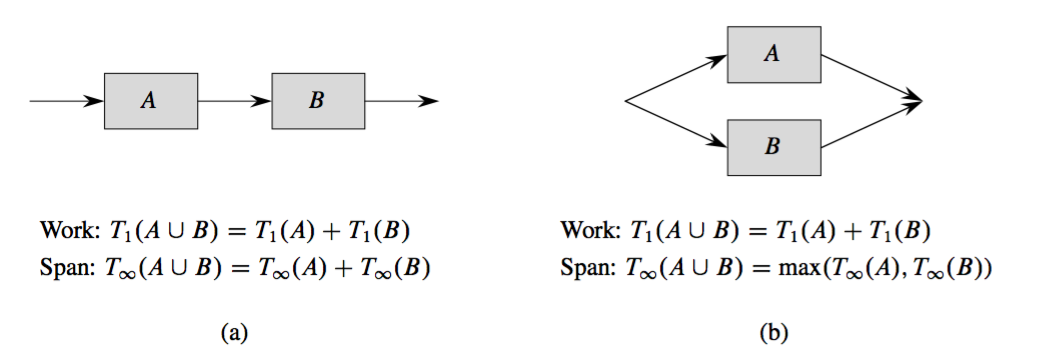
\includegraphics{./notes/immagini/l25-fig1.png}
\caption{}
\end{figure}

Se due computazioni devono essere eseguite in sequenza la durata è la
somma dei Tinf delle due compitazioni. Se invece possono essere eseguiti
in parallelo, la durata è il massimo dei due Tinf.

\subsection{Loop paralleli}\label{loop-paralleli}

Moltiplicazione di un vettore per una matrice di dimensione \emph{nxn}

\begin{verbatim}
\Function{MatVec}{$A,x$}
    \State $n \gets A.rows$
    \State $y\gets Vec(n)$
    \State \textbf{parallel}
    \For{$i = 1 \text{ to } n$}
        \State $y_i \gets 0$
    \EndFor
    \State \textbf{parallel}
    \For{$i = 1 \text{ to } n$}
         \For{$j = 1 \text{ to } n$}
            \State $y_i \gets y_i + a_{i,j}x_j$
        \EndFor
    \EndFor
\end{verbatim}

Per quanto riguarda il lavoro si ha T1(n) = Tetha(n\^{}2).

La durata invece Tinf(n) si ha che il primo blocco \textbf{parallel} ha
durata Theta(log(n)), perché il ciclo di azzeramento viene ottimizzato
in modo analogo dalla piattaforma parallela in qualcosa di simile:

\begin{verbatim}
Azzera(y,i,j)
if i = j
    y_i = 0
else 
    m = floor(i+j/2)
    spawn azzera(y,i,m)
    azzera(y,m+1,j)
    sync
\end{verbatim}

Il lavoro di questa procedura in funzione di n = j-i+1 è T1(n)= 2T1(n/2)
+ C = Theta(n). Tinf(n) è invece unguale a Tinf(n/2)+C = Theta(log(n))
che deve essere sommata alla durata del blocco, che in questo caso è
costante.

In modo simile a prima il secondo blocco ha complessità Theta(log(n)) +
Theta(n) = Theta(n).

Si ha quindi che quando c'è un parallel c'è sempre una costante log(n)
da sommare alla complessità a causa dell'implementazione del for.

Tinf di tutto l'algoritmo è quindi Theta(n).

\subsection{Race condition}\label{race-condition}

Se l'esecuzione dell'algortimo fornisce sempre lo stesso risultato viene
detto \textbf{deterministico} e questo avviene quando l'ordine di
esecuzione degli strand non è influente sul risultato.

Se invece l'ordine è influente sul risultato si ha che l'agoritmo è
\textbf{non deterministo} e questo può essere causato da delle
\textbf{race condition} ovvero quando due strand eseguiti in paralleli
accedono alla stessa locazione di memoria.

\subsection{Una lezione di scacchi}\label{una-lezione-di-scacchi}

Un algoritmo parallelo è stato progettato per lavorare con p = 32 e con
un T32 = 65 secondi.

Si è poi riusciti a ridurre il tempo di esecuzione a T'32 = 40 secondi.

Tuttavia una volta eseguito il codice con p = 512 la seconda versione
dell'algoritmo è risultata meno performante.

La versione originale aveva T1 = 2048 e Tinf = 1, mentre quella
modificata aveva T'1 = 1024 e Tinf 8. Ovvero la seconda versione ha
dimezzato il lavoro, ma ha aumentato la durata.

Per il programma originale, utilizzando Tp = T1/p + Tinf:

T32 = 2048/32 +1 = 65 T'32 = 1024/32 +8 = 40

mentre

T512 = 2048/512 + 1 = 5 T512 = 1024/512 + 8 = 10

Morale della favola, diminuire il lavoro non sempre porta ad una
riduzione della durata.

\section{Merge Sort}\label{merge-sort}

La versione sequenziale dell'algoritmo prende un array \emph{A} e due
indici \emph{p} e \emph{r} e deve ordinare la porzione dell'array
compresa tra \emph{p} e \emph{r}.

\begin{verbatim}
\Function{MergeSort'}{$A,p,r$}
\If{$p < r$}
    \State $q \gets floor(p+r/2)$
    \State \textbf{spawn } \texttt{MergeSort'}$(A,p,q)$
    \State \texttt{MergeSort'}$(A,q+1,r)$
    \State \textbf{sync}
    \State \texttt{Merge}$(A,p,q,r)$
\EndIf
\EndFunction
\end{verbatim}

Il lavoro T1(n) è Theta(n log(n)) che deriva dalla versione sequenziale
del \texttt{MergeSort}.

La durata è invece uguale ad un tempo costante, più la massima durata
delle chiamata ricorsive (che possono essere considerate uguali) più la
durata del merge, che se viene fatto in modo sequenziale è Theta(n). Si
ha quindi che Tinf = Tinf(n/2) + Theta(n) = Theta(n) (\emph{per il
metodo dell'esperto o qualcosa del genere}).

Il parallelismo di questo algoritmo risulta quindi essere Theta(log(n))
che non risulta essere buono.

\begin{verbatim}
To sort 10 million elements, for example, it might achieve linear speedup on a few processors, but it would not scale up effectively to hundreds of processors.
\end{verbatim}

Per aumentare il parallelismo è necessario rendere parallela anche la
funzione \texttt{Merge}.

\begin{figure}[htbp]
\centering
\includegraphics{./notes/immagini/l25-fig2.png}
\caption{}
\end{figure}

Supponiamo che nell'array \emph{T} risultante dalle due chiamate
ricorsive ci siano due porzioni ordinate che vanno rispettaivamente da
\emph{p1} a \emph{r1} e da \emph{p2} a \emph{r2}.

L'idea è quella di prendere la parte più lunga dei due segmenti. Se
questa è lunga 0, sono entrambi vuoti e non è necessario fare niente.

Se invece è più lunga di 0, viene calcolato l'indice \emph{q1} medio,
ovvero l'elemento centrale della sequenza, il quale avrà un certo valore
\emph{x}.

La seconda sequenza può quindi essere divisa in altre due sottosequenze
contenenti solo valori minori di \emph{x} e un'altra con tutti i valori
\emph{\textgreater{}= x}. Il primo elemento \emph{\textgreater{}= x}
avrà un certo indice \emph{q2}. Questo può essere fatto con il binary
search in un tempo logaritmico.

Da notare che \emph{q2} può essere uguale a \emph{p2} se sono tutti
maggiori uguali o a \emph{r2+1} se sono tutti minori.

Si sa quindi che una volta ordinato il vettore, l'elemento \emph{x} si
troverà nella posizione \emph{q3 = p3 + (q1-p1) + (q2-p2)} e può essere
già scritto.

Si possono poi unire ricorsivamente tutti gli elementi minori di
\emph{x}, ovvero quelli che vanno da \emph{p1} a \emph{q1-1} e da
\emph{p2} a \emph{q2-1} , e tutti quelli maggiori uguali di \emph{x},
ovvero quelli che vanno da \emph{q1} a \emph{r1} e da \emph{q2} a
\emph{r2}.

Dal momento che i primmi andranno a finire nelle posizioni da \emph{q3}
a \emph{q3-1} e i secondi andranno a finire nelle posizioni da
\emph{q3+1} a \emph{r3}, le due chiamate ricorsive possono essere
parallelizzate.

%\appendix


%----------------------------------------------------------------------------------------
% BIBLIOGRAPHY
%----------------------------------------------------------------------------------------
%\bibliographystyle{unsrt}
%\bibliography{sample}
%----------------------------------------------------------------------------------------

\end{document}